\documentclass[11pt]{article}
\usepackage[utf8]{inputenc}
\usepackage[a4paper,margin=24mm,headheight=15pt]{geometry}
\usepackage{amsmath,amssymb,mathtools}
\usepackage{xcolor}
\usepackage{array,longtable,booktabs}
\usepackage{graphicx}
\usepackage{float}
\floatplacement{figure}{H}
\usepackage{fancyvrb}
\usepackage{fancyhdr}
\usepackage{needspace}
\usepackage[colorlinks=true,linkcolor=blue!45!black,urlcolor=blue!60!black]{hyperref}
\hypersetup{pdftitle={Point particles, cone cuts, and extremal limits},pdfauthor={Research note for anshM123/MAJOR}}
\setlength{\emergencystretch}{3em}
\setlength{\parindent}{0pt}
\setlength{\parskip}{4pt plus 1pt}
\setcounter{secnumdepth}{-1000}
\setcounter{tocdepth}{1}
\providecommand{\tightlist}{\setlength{\itemsep}{1pt}\setlength{\parskip}{0pt}}
\providecommand{\passthrough}[1]{#1}
\providecommand{\pandocbounded}[1]{#1}
\renewcommand{\labelitemi}{\(\bullet\)}
\DefineVerbatimEnvironment{Highlighting}{Verbatim}{fontsize=\small}
\newenvironment{Shaded}{}{}
\newcommand{\KeywordTok}[1]{#1}
\newcommand{\ExtensionTok}[1]{#1}
\newcommand{\NormalTok}[1]{#1}
\newcommand{\OperatorTok}[1]{#1}
\newcommand{\StringTok}[1]{#1}
\newcommand{\CommentTok}[1]{#1}
\DeclareUnicodeCharacter{039B}{\ensuremath{\Lambda}}
\DeclareUnicodeCharacter{03A3}{\ensuremath{\Sigma}}
\DeclareUnicodeCharacter{03B3}{\ensuremath{\gamma}}
\DeclareUnicodeCharacter{03B4}{\ensuremath{\delta}}
\DeclareUnicodeCharacter{03B5}{\ensuremath{\epsilon}}
\DeclareUnicodeCharacter{03B7}{\ensuremath{\eta}}
\DeclareUnicodeCharacter{03BB}{\ensuremath{\lambda}}
\DeclareUnicodeCharacter{03C0}{\ensuremath{\pi}}
\DeclareUnicodeCharacter{03C1}{\ensuremath{\rho}}
\DeclareUnicodeCharacter{03C3}{\ensuremath{\sigma}}
\DeclareUnicodeCharacter{03C4}{\ensuremath{\tau}}
\DeclareUnicodeCharacter{03C6}{\ensuremath{\phi}}
\DeclareUnicodeCharacter{03C7}{\ensuremath{\chi}}
\DeclareUnicodeCharacter{00B9}{\ensuremath{{}^1}}
\DeclareUnicodeCharacter{00B2}{\ensuremath{{}^2}}
\DeclareUnicodeCharacter{00B1}{\ensuremath{\pm}}
\DeclareUnicodeCharacter{207B}{\ensuremath{{}^{-}}}
\DeclareUnicodeCharacter{2080}{\ensuremath{{}_0}}
\DeclareUnicodeCharacter{2083}{\ensuremath{{}_3}}
\DeclareUnicodeCharacter{2192}{\ensuremath{\to}}
\DeclareUnicodeCharacter{2208}{\ensuremath{\in}}
\DeclareUnicodeCharacter{220E}{\ensuremath{\square}}
\DeclareUnicodeCharacter{2212}{\ensuremath{-}}
\DeclareUnicodeCharacter{2218}{\ensuremath{\circ}}
\DeclareUnicodeCharacter{221E}{\ensuremath{\infty}}
\DeclareUnicodeCharacter{2229}{\ensuremath{\cap}}
\DeclareUnicodeCharacter{2260}{\ensuremath{\ne}}
\DeclareUnicodeCharacter{2261}{\ensuremath{\equiv}}
\DeclareUnicodeCharacter{2264}{\ensuremath{\le}}
\DeclareUnicodeCharacter{2265}{\ensuremath{\ge}}
\DeclareUnicodeCharacter{226A}{\ensuremath{\ll}}
\DeclareUnicodeCharacter{2282}{\ensuremath{\subset}}
\DeclareUnicodeCharacter{00D7}{\ensuremath{\times}}
\DeclareUnicodeCharacter{00B7}{\ensuremath{\cdot}}
\renewcommand{\textbar}{\ensuremath{|}}
\renewcommand{\textgreater}{\ensuremath{>}}
\renewcommand{\textless}{\ensuremath{<}}
\pagestyle{fancy}
\fancyhf{}
\fancyhead[L]{\small Particles and entropy cones}
\fancyhead[R]{\small Proof and validation}
\fancyfoot[C]{\thepage}
\title{\bfseries Point particles, cone cuts,\\and extremal limits}
\author{Research dossier for \texttt{anshM123/MAJOR}}
\date{28 November 2026}
\DeclareUnicodeCharacter{0394}{\ensuremath{\Delta}}
\DeclareUnicodeCharacter{0393}{\ensuremath{\Gamma}}
\DeclareUnicodeCharacter{0398}{\ensuremath{\Theta}}
\DeclareUnicodeCharacter{03B1}{\ensuremath{\alpha}}
\DeclareUnicodeCharacter{03B2}{\ensuremath{\beta}}
\DeclareUnicodeCharacter{03B8}{\ensuremath{\theta}}
\DeclareUnicodeCharacter{03BC}{\ensuremath{\mu}}
\DeclareUnicodeCharacter{03BD}{\ensuremath{\nu}}
\DeclareUnicodeCharacter{03BE}{\ensuremath{\xi}}
\DeclareUnicodeCharacter{03C8}{\ensuremath{\psi}}
\DeclareUnicodeCharacter{03C9}{\ensuremath{\omega}}
\DeclareUnicodeCharacter{2202}{\ensuremath{\partial}}
\DeclareUnicodeCharacter{2200}{\ensuremath{\forall}}
\DeclareUnicodeCharacter{2203}{\ensuremath{\exists}}
\DeclareUnicodeCharacter{2205}{\ensuremath{\emptyset}}
\DeclareUnicodeCharacter{2211}{\ensuremath{\sum}}
\DeclareUnicodeCharacter{2248}{\ensuremath{\approx}}
\DeclareUnicodeCharacter{2286}{\ensuremath{\subseteq}}
\DeclareUnicodeCharacter{21D2}{\ensuremath{\Rightarrow}}
\DeclareUnicodeCharacter{2194}{\ensuremath{\leftrightarrow}}
\DeclareUnicodeCharacter{211D}{\ensuremath{\mathbb{R}}}
\DeclareUnicodeCharacter{2124}{\ensuremath{\mathbb{Z}}}
\DeclareUnicodeCharacter{2115}{\ensuremath{\mathbb{N}}}
\DeclareUnicodeCharacter{2081}{\ensuremath{{}_1}}
\DeclareUnicodeCharacter{2082}{\ensuremath{{}_2}}
\DeclareUnicodeCharacter{2084}{\ensuremath{{}_4}}
\DeclareUnicodeCharacter{2070}{\ensuremath{{}^0}}
\DeclareUnicodeCharacter{2074}{\ensuremath{{}^4}}
\renewcommand{\textquotesingle}{\char39}
\renewcommand{\textasciigrave}{\char96}
\renewcommand{\textasciitilde}{\ensuremath{\sim}}
\renewcommand{\textasciicircum}{\ensuremath{\wedge}}
\begin{document}
\maketitle
\thispagestyle{empty}
\begin{abstract}
We extend the standing vacuum entropy-cone theorem to compatible finite
spinless orbifold quotients, using invariant graph minima and smooth
orbifold homology slices. A separate funnel-replacement argument proves
full-cone membership for the relaxed common-class functional of marked
hyperbolic cone metrics at arbitrary cone angles; below angle \(\pi\),
all relevant geodesic lengths are preserved exactly. We also exhibit a
static positive-mass cone whose HRT length differs from the proposed
chiral-cone half-sum, so this mathematical result cannot be imported
unchanged into a general particle-spacetime theorem. For the explicit
two-massless-particle formation kernel, we prove a positive kinematic
measure at every boundary time and control the physical single-interval
branch thresholds algebraically. The matching model passes all 372
five-party facets in 2,169,504 numerical evaluations. Quantitative extremal
BTZ limits and an unwrapped-exterior HRT theorem complete the package.
The unrestricted collision multicurve realization problem remains open.
\end{abstract}
\vspace{6pt}
\tableofcontents
\clearpage

\Needspace{8\baselineskip}
\section{Results and precise scope}\label{results-and-precise-scope}

Research extension, 28 November 2026, based on repository revision
\texttt{acda6f59a240} and its standing vacuum Theorem H, smooth-slice
theorem, and exact full-cone arrangement construction.

\Needspace{6\baselineskip}
\subsection{What this work
establishes}\label{what-this-work-establishes}

The general collision theorem is not established here, and the proposed
arbitrary-angle chiral-cone HRT identification is false in an explicit
static example. There is an actual matter extension with no new maximin
assumption, an exact all-time positivity theorem for the explicit
two-particle interval kernel, and a quantitative treatment of the
extremal limit.

\begin{longtable}[]{@{}
  >{\raggedright\arraybackslash}p{(\columnwidth - 2\tabcolsep) * \real{0.5000}}
  >{\raggedright\arraybackslash}p{(\columnwidth - 2\tabcolsep) * \real{0.5000}}@{}}
\toprule\noalign{}
\begin{minipage}[b]{\linewidth}\raggedright
Result
\end{minipage} & \begin{minipage}[b]{\linewidth}\raggedright
Status and scope
\end{minipage} \\
\midrule\noalign{}
\endhead
\bottomrule\noalign{}
\endlastfoot
Finite spinless orbifold particles & HRT/full-cone descent from a
compatible smooth vacuum cover; arbitrary finite party number and
allowed boundary times \\
Smooth homology slice through quotient HRT & Proved in orbifold charts,
including avoidance of every particle axis \\
Filled-class cone Crofton & False at every positive-mass cone angle; an
explicit positive-measure counterexample is supplied \\
Arbitrary-angle marked cone functional & Full RT-cone theorem for the
relaxed common-class length infimum \\
Cone angles below pi & Exact attained geodesic-length functional, via
uniform collar exclusion and funnel replacement \\
Naive arbitrary-angle chiral-cone HRT identity & Explicitly false on a
tilted boundary slice of a static spinless cone \\
Ordinary common cusp ends & Exact positive-graph theorem for the
geometric cut functional, with unmarked cusp colors \\
Compact extremal BTZ & Full-cone theorem for the nonextremal limiting
entropy functional, with a uniform error bound \\
Unwrapped extremal BTZ & Actual bounded-interval HRT full-cone theorem
using the explicit Poincare patch \\
Two-massless-particle formation kernel & Exact positive kinematic
measure at all BTZ boundary times \\
Two-particle multiparty matching functional & Exact all-party RT-cone
theorem and a 372-facet numerical audit \\
Physical HRT through collisions for every union & Still requires
simultaneous admissibility/acausality; not inferred from endpoint
noncrossing \\
\end{longtable}

All HRT claims are at the classical area/length order. The endpoint
cutoff or positive endpoint Bell terms are retained for full-cone
membership. Endpoint-balanced inequalities also apply directly to the
renormalized finite parts. The standing vacuum theorems are inputs to
the new deductions; this addition is not an independent verification of
the entire repository.

\Needspace{6\baselineskip}
\subsection{The unconditional matter
result}\label{the-unconditional-matter-result}

Let a finite orientation- and time-orientation-preserving group \(F\)
act isometrically on a smooth vacuum spacetime \(\widetilde M\) covered
by the standing theorem. Assume compatibility with the marked chiral
surfaces and the smooth conformal double, and no boundary fixed points.
In the quotient \(M=\widetilde M/F\), include the timelike fixed axes as
ordinary filled spinless orbifold particles. For every boundary region,

\[
S_M(A)=\frac{1}{|F|}\,S_{\widetilde M}(\widetilde A),
\]

where \(\widetilde A\) is the full preimage and cutoffs are compatible.
One finite positive-capacity graph represents every party union.

The proof does not assume the cover minimizer is unique or symmetric.
Submodularity of graph cuts provides an invariant minimum. An invariant
frontier class then gives an invariant geodesic cut. Averaging a Cauchy
temporal function constructs an invariant smooth slice through it. Its
homology-side coloring is invariant, so a nontrivial stabilizer cannot
fix a point of the curve: a rotation cannot preserve the tangent
half-plane. This includes the order-two case.

The resulting particle angles are \(2\pi/n_i\), \(n_i\ge2\). These are
genuine positive-deficit particles, but the angles are not dense in
\((0,2\pi)\). Finite Lorentz isotropy fixes a single timelike axis; this
theorem therefore does not include collision vertices.

Full proof: \texttt{FINITE\_\allowbreak ORBIFOLD\_\allowbreak THEOREM.md}.

\Needspace{6\baselineskip}
\subsection{The cone issue is a topology issue, not a measure-zero
exception}\label{the-cone-issue-is-a-topology-issue-not-a-measure-zero-exception}

On a cone with any \(0<\theta<2\pi\), a globally minimizing anchored cut
can be crossed twice by an open family of regular embedded test
geodesics, while their geometric intersection number in the filled disk
is zero. Neither geodesic hits the tip. Thus removing cone-hitting
geodesics does not restore the original intersection formula, even below
angle \(\pi\).

Particles should be filled for \textbf{homology}, while their marks
remain in the \textbf{isotopy classes}. The finite-cover theorem
supplies one rigorous way around the resulting analytic problem.

Proof and figure: \texttt{CONE\_\allowbreak INTERSECTION\_\allowbreak AUDIT.md},
\texttt{figures/cone\_\allowbreak bigon.pdf}.

\Needspace{5\baselineskip}
\subsubsection{A replacement proof for every cone
angle}\label{a-replacement-proof-for-every-cone-angle}

The Crofton failure can be bypassed. Replace a radius-\(a\) cone
neighborhood by a smooth negatively curved funnel, with its homology
color free. The replacement admits a marking-preserving 1-Lipschitz map
back to the old punctured cone. Consequently every marked class length
is bounded below by its old infimum. Any fixed regular comparison curve
misses all sufficiently small collars, giving the matching upper bound
as \(a\to0\).

Choose one nearly optimal common class for each required region, and
then nearly optimal representatives in each metric. This proves
convergence of the common-class infimum without interchanging an
uncontrolled infinite minimum and a limit. The smooth replacements have
positive graph models; the endpoint constants are independent of \(a\).
Closedness of the RT cone therefore proves full-cone membership of the
relaxed marked-cone functional at every angle in \((0,2\pi)\), and
mathematically beyond that range as well.

Below angle \(\pi\), every embedded complete regular geodesic avoids a
uniform collar, \[
r<\operatorname{arctanh}\!\left(\tanh R_{\rm collar}\cos(\theta/2)\right).
\] Replacing the cones inside those collars preserves all reduced simple
geodesic lengths exactly. No relaxation or limit is then needed.

These are mathematical functional theorems. They become physical entropy
theorems wherever the HRT/common-class identification is independently
established. The proofs are in
\texttt{ALL\_\allowbreak ANGLE\_\allowbreak RELAXED\_\allowbreak FUNCTIONAL.md} and
\texttt{SMALL\_\allowbreak ANGLE\_\allowbreak FUNCTIONAL\_\allowbreak THEOREM.md};
\texttt{COMMON\_\allowbreak SIDE\_\allowbreak ROUNDING.md} records a further local improvement
lemma and its precise limitation.

\Needspace{6\baselineskip}
\subsection{Exact positivity in the formation
example}\label{exact-positivity-in-the-formation-example}

For the explicit equal-time interval kernel of arXiv:1706.07390, write
\(X=e^{Ra}<1<Y=e^{Rb}\), \(Z=e^{Rt}\), and \(E=\coth(\pi R/2)\). The
crossing expression factors as

\[
D_{\mathrm c}=\log\frac{F_1F_2}{XYZ^2},\qquad
\begin{cases}
F_1=E(X-Z)(Y-Z)+Z(Y-X),\\
F_2=E(XZ-1)(YZ-1)+Z(Y-X).
\end{cases}
\]

Both factors are strictly positive on every shortest-arc chart. Their
bilinear determinants equal \(Z^2\). Moreover, if
\(h=D_{\mathrm c}-D_{\mathrm d}\), then \(h_a\ge0\) and \(h_b\le0\).
Concave smoothing of the branch minimum therefore proves

\[
\partial_a\partial_b\min(D_{\mathrm c},D_{\mathrm d})\ge0
\]

as a distribution, including singular switching loci. Injection and
antipodal seams also contribute no negative measure. The finite disk
graph theorem then places the noncrossing-matching functional in the
full RT cone at every time, for every party number.

This settles the algebraic/current part for the explicit collision
kernel. It does not silently identify every minimizing matching with a
physical HRT multicurve. \texttt{COLLISION\_\allowbreak ADMISSIBILITY.md} records
the further geometric analysis and the precise remaining condition.

The numerical audit evaluates 2,169,504 facet values from 5,832 matching
vectors. All 372 five-party facets pass within \(10^{-10}\); the minimum
is \(-1.42\times10^{-13}\). The analytic theorem, rather than this
sample, establishes the all-time assertion for the matching functional.

\Needspace{6\baselineskip}
\subsection{A physical counterexample to the assumed chiral
identity}\label{a-physical-counterexample-to-the-assumed-chiral-identity}

In static conical AdS with \(\theta=3\pi/2\), choose
\(\Delta\phi=11\pi/16\) and \(\Delta t=9\pi/16\). These endpoints fit on
a spacelike boundary Cauchy curve. The direct spacetime geodesic stays
in an embedded angular sector, misses the particle, is globally acausal,
and admits a Cauchy homology slice. Its length is \[
L_{\rm HRT}=\log\!\left[4\sin(5\pi/8)\sin(\pi/16)\right]
=-0.3271718686\ldots.
\] The proposed chiral cone classes have sweeps \(5\pi/4\) and
\(\pi/8\). The first has no regular hyperbolic-cone geodesic. Relaxing
its length to the cone-hitting infimum gives instead \[
F_{\rm rel}=\log\!\left[4\sin(\pi/16)\right]
=-0.2479982767\ldots.
\] The exact mismatch is \(-\log\sin(5\pi/8)>0\), in identical endpoint
normalization. The second embedded branch is more expensive in both
prescriptions. Its mismatch is different, so a common endpoint
counterterm cannot fix both class lengths.

This disproves the proposed large-angle identification, not an entropy
inequality. The all-angle mathematical functional theorem remains true,
but a physical particle theorem needs a different argument. See
\texttt{TILTED\_\allowbreak CONE\_\allowbreak COUNTEREXAMPLE.md} and its 80-digit
checker/figure.

\Needspace{6\baselineskip}
\subsection{What changes at
extremality}\label{what-changes-at-extremality}

For \(\alpha=(r_+-r_-)/2\to0\), fixed \(\beta=(r_++r_-)/2>0\), boundary
circumference \(P\), and a union with \(2k\) endpoints,

\[
0\le F_{\alpha,\beta}(A)-F_{0,\beta}(A)
\le k\frac{\alpha^2P^2}{6}+P\alpha.
\]

Only two same-boundary embedded arc windings are possible; the candidate
cut set is finite. Closedness of the RT cone gives the limiting
full-cone theorem. However, the genuine hyperbolic-parabolic quotient
has no invariant AdS geodesic in its peripheral class. A positive
limiting core cost is not an attained extremal horizon circle. The
unwrapped exterior has no compact core requirement and admits an actual
bounded-interval HRT theorem.

Full proofs and conventions: \texttt{CUSPS\_\allowbreak EXTREMAL\_\allowbreak BTZ.md}.

\Needspace{6\baselineskip}
\subsection{Reproduction and file map}\label{reproduction-and-file-map}

From this directory, with the dependencies in \texttt{requirements.txt}:

\begin{verbatim}
python code/check_equivariant_mincut.py
python code/check_cone_bigon.py
python code/check_extremal_limit.py
python code/check_tilted_cone.py
python code/bilocal_collision.py \
  --facets data/facets_n5_all372.json \
  --output collision_reproduction
\end{verbatim}

The first three checkers write their diagnostic outputs beside their
scripts; archived run outputs are in \texttt{data/}. The final command
writes its JSON and figures to the named directory. No computation
contacts a remote service. The facet catalogue includes its original
author/source URL and subset ordering.

The exact finite-group checker covers 321 examples, including asymmetric
degenerate minima, fixed vertices, and stabilized edges. The extremal
checker includes exact matrix and horizon-acceleration identities,
complete finite annular-cut enumeration, and 155 convergence-bound
instances. The cone checker verifies the analytic counterexample at
angles on both sides of \(\pi\). None of these finite tests replaces its
associated proof.

\texttt{OPEN\_\allowbreak GAPS\_\allowbreak UPDATE.md} gives the precise status update supported
by the work. The source audit in \texttt{SPACETIME\_\allowbreak AUDIT.md} explains
the distinct issues posed by spin, elliptic particles, massless
particles, and collisions. The presented results do not justify the
blanket headline that arbitrary particle collisions never leave the
static cone.

\clearpage

\Needspace{8\baselineskip}
\section{Finite-orbifold HRT and graph
descent}\label{finite-orbifold-hrt-and-graph-descent}

Research checkpoint, 28 November 2026. This result uses the standing
vacuum Theorem H and the equivariant form of the arrangement
construction in \texttt{PROOFS.md} and \texttt{fullcone/FULLCONE.md}, at
repository revision \texttt{acda6f59a240}. It adds no maximin
assumption.

\Needspace{6\baselineskip}
\subsection{1. Precise statement}\label{precise-statement}

Let \(\widetilde M\) be a smooth vacuum spacetime in the class covered
by Theorem H and the full-cone arrangement theorem. Let a finite group
\(F\), of order \(q\), act by orientation- and
time-orientation-preserving isometries. Assume the action respects the
conformal completion and its double: each group element extends smoothly
and conformally to the double, preserves its time orientation, and
commutes with boundary reflection. Assume also that its induced actions
on the two marked chiral hyperbolic surfaces are isometries in the
common topological marking. Take the quotient \(M=\widetilde M/F\),
including its fixed timelike axes as orbifold particle worldlines.
Require no fixed points on the conformal boundary.

Let \(A_1,\ldots,A_N\) be disjoint boundary regions on a boundary Cauchy
slice of \(M\), and let \(\widetilde A_i\) be their full preimages. Use
compatible quotient/lifted endpoint cutoffs. A quotient HRT candidate is
an embedded regular-locus spacelike extremal multicurve with a homology
region on an acausal orbifold Cauchy slice; cone points are filled for
that homology.

\textbf{Theorem.} For every party union \(A\),

\[
 S_M(A)=q^{-1}S_{\widetilde M}(\widetilde A).
 \tag{1}
\]

There is one finite positive-capacity graph representing all the
quotient entropies simultaneously. Thus the quotient vector lies in the
full static RT cone, with precisely the endpoint/UV convention of the
cover theorem. In particular, regulated vectors are positive-graph
vectors for all sufficiently small compatible cutoffs, for which the
cover's endpoint Bell capacities are nonnegative. The conclusion holds
for any finite number of parties and arbitrary boundary Cauchy time
profiles. The quotient HRT minimum is attained on an acausal Cauchy
slice that is smooth and uniformly spacelike in orbifold charts of the
conformal completion; the minimizing curves avoid every particle
worldline. The uniform margin depends on the geometry and the cut, as in
the cover theorem.

This is a theorem for finite orbifold quotients, not for arbitrary cone
angles, spinning particles, or collisions.

\Needspace{6\baselineskip}
\subsection{2. An equivariant arrangement graph
exists}\label{an-equivariant-arrangement-graph-exists}

All endpoint lifts form a finite \(F\)-invariant set. For each required
boundary union choose a minimizing cut class in the cover. In the
arrangement construction include that class and all of its
\(F\)-translates. The resulting finite arrangement in the reference
chiral hyperbolic surface is \(F\)-invariant. Adding these translates
does not invalidate the graph proof: every selected optimum remains an
arrangement cut, and the lower bound applies to every cut of the refined
arrangement.

The total renormalized intersection functional is \(F\)-invariant, since
the group acts by isometries of each chiral metric. Choose the auxiliary
test-geodesic measure equivariantly. Equivalently, replace any realizing
measure by its finite average \(q^{-1}\sum_{g\in F}g_*\nu\). Its
intersection pairing with any class is unchanged. Endpoint terms can
likewise be chosen constant on endpoint orbits, because the cutoff is
lifted from the quotient.

Consequently each arrangement-edge capacity equals the capacity of each
of its translates. Add the endpoint Bell edges equivariantly. The
resulting finite graph \(\mathcal G\) carries an \(F\)-action by graph
automorphisms; all boundary labels are \(F\)-invariant. The complete
cover entropy vector for the lifted parties is its mincut vector.

\Needspace{6\baselineskip}
\subsection{3. A minimum cut can be chosen
invariant}\label{a-minimum-cut-can-be-chosen-invariant}

For a set \(U\) of graph vertices, let \(c(U)\) be its undirected cut
capacity. Nonnegative edge capacities imply

\[
 c(U\cup V)+c(U\cap V)\le c(U)+c(V).
 \tag{2}
\]

If \(U,V\) are both minimum cuts with the same fixed terminal labels,
their union and intersection are admissible and each has capacity at
least the minimum \(m\). Equation (2) forces both to have capacity
exactly \(m\).

Starting from any minimum cut \(U\), form

\[
 U_F=\bigcup_{g\in F}gU.
 \tag{3}
\]

Every \(gU\) is a minimum cut with the same labels. Finite iteration of
(2) shows that \(U_F\) is a minimum cut and is \(F\)-invariant. This
argument does not assume a unique minimum or strict inequalities.

\Needspace{6\baselineskip}
\subsection{4. From the invariant graph cut to an invariant topological
cut}\label{from-the-invariant-graph-cut-to-an-invariant-topological-cut}

First ignore the added endpoint Bell edges, whose contribution is fixed
by the boundary union. The selected arrangement cells of \(U_F\) form an
invariant, possibly nonsmooth homology region. Smooth its frontier
equivariantly in small disks around arrangement vertices, using an
\(F\)-invariant auxiliary Riemannian metric and orbitwise equal radii. A
regular-neighborhood construction chooses the same resolution at all
vertices in an orbit and is automatically invariant at vertices with
nontrivial stabilizers. At a fixed vertex, filling a small invariant
disk and rounding the unselected sectors, or the complementary
construction, provides such a resolution. Endpoint half-disks are
treated with their marked endpoint fixed; the group acts freely on these
endpoints.

The resolutions give an embedded cut class \(c\) with the required
trace. Its isotopy class is invariant. Inessential loops and redundant
parallel boundary pairs are removed in their full group orbits; this is
the usual reduction of a cut class and preserves the homology trace.

The standing cover construction uses a measure absolutely continuous
with respect to Liouville measure on proper arc geodesics: almost every
test geodesic has both endpoints outside the limit set and the marked
endpoint orbits, meets the finite arrangement transversely in finitely
many points, and hits no arrangement vertex. Finite averaging preserves
these facts. For each such proper geodesic, sufficiently small smoothing
disks and endpoint horoballs are disjoint from it and do not change its
crossings with the frontier. Merely avoiding a vertex would not suffice
for an arbitrary recurrent complete geodesic; the properness supplied by
the cover's test measure is used here. The intersection number of its
test class with \(c\) is therefore no larger than its crossings with the
original selected arrangement edges. The class is constant for all
sufficiently small resolutions. Integrating the pointwise inequality
gives

\[
 \mathcal L(c)\le \operatorname{cap}(U_F)=S_{\widetilde M}(\widetilde A).
 \tag{4}
\]

Here \(\mathcal L\) includes the same endpoint terms and the factor
\(1/(4G_N)\) as the entropy functional. The cover's minimum-over-classes
theorem gives the reverse inequality. Thus \(c\) is a minimizing cover
class.

Every reduced simple class has its unique chiral geodesic
representatives, and Theorem H gives its unique spacetime geodesic
multicurve \(K\) in the vacuum domain. Isometries carry these
representatives to the representatives of the transformed classes. Since
\(c\) is invariant, \(K\) is invariant. Theorem H supplies acausality,
embeddedness, and a homology Cauchy slice.

\Needspace{6\baselineskip}
\subsection{5. An invariant smooth Cauchy slice through the
curve}\label{an-invariant-smooth-cauchy-slice-through-the-curve}

Work first in the smooth conformal double of the cover. The finite group
action extends to that double and commutes with boundary reflection. It
preserves the causal cones; isometry of an arbitrarily selected
conformal representative is unnecessary. If an invariant representative
is desired, average a reflection-invariant representative as
\(\bar g_F=q^{-1}\sum_g g^*\bar g\). The summands are pointwise positive
conformal multiples, so the result is a smooth Lorentz metric with the
same cones, invariant under both the group and reflection. The doubled
compact curve is invariant and acausal. The cover's smooth-slice theorem
supplies a smooth spacelike Cauchy surface \(S\) containing it.

Bernal--Sanchez, arXiv:gr-qc/0512095, Theorem 1.2, supplies a smooth
Cauchy temporal function \(T\) with \(S=T^{-1}(0)\). Define

\[
 T_F(x)=q^{-1}\sum_{g\in F}T(gx).
 \tag{5}
\]

Every summand has a past-directed timelike differential (equivalently
the appropriate directed timelike gradient). The timelike covector cone
is convex, so \(T_F\) is temporal. Along any future-inextendible causal
curve, each of the finitely many summands tends to \(+\infty\); along
any past-inextendible one, each tends to \(-\infty\). Thus \(T_F\) is
Cauchy. Since \(K\) is invariant and \(T\) vanishes on it, \(T_F\)
vanishes on it.

The level surface \(S_F=T_F^{-1}(0)\) is an invariant smooth spacelike
Cauchy surface through \(K\). Restrict it to the original conformal
half. Transversality to the timelike conformal boundary and the Cauchy
property follow exactly as in Proposition S+ of the cover theorem. The
restricted surface is compact by that proposition's compactness
argument. Strict positivity on its compact auxiliary unit tangent bundle
therefore supplies a uniform spacelike margin; this descends in orbifold
charts because the covering group is finite.

Transport a homology region for \(K\) from the original slice to this
one along a complete future timelike flow tangent to the conformal
boundary. The transport fixes \(K\) and preserves its marked boundary
trace. No equivariance of that transport is needed for the next
argument.

\Needspace{6\baselineskip}
\subsection{6. The homology region is invariant and the curve misses
every
axis}\label{the-homology-region-is-invariant-and-the-curve-misses-every-axis}

\textbf{Coloring lemma.} On a connected surface with nonempty boundary,
a specified embedded reduced cut multicurve and its boundary trace
determine the homology-region coloring uniquely. Indeed, the symmetric
difference of two such colorings has no jump across any cut component,
so its indicator is locally constant on the entire connected surface. It
vanishes in a boundary collar where the traces agree, hence vanishes
everywhere.

Apply this to the region \(R\subset S_F\) just constructed. Both \(gR\)
and \(R\) have frontier \(K\) and the same invariant boundary trace, so
the coloring lemma implies \(gR=R\).

Suppose \(p\in K\) were fixed by a nonidentity deck element. On the
invariant spacelike plane \(T_pS_F\), its linear action is a nontrivial
finite rotation. Indeed it preserves the future normal and the spatial
orientation; an identity spatial derivative would be an identity ambient
derivative, and an isometry fixing a point with identity derivative is
the identity on the connected spacetime. Embeddedness makes the tangent
cone of \(R\) at \(p\) one of the two closed half-planes bounded by
\(T_pK\). No nontrivial rotation preserves a half-plane. This
contradicts invariance of \(R\).

This explicitly includes isotropy order two: a rotation by \(\pi\)
preserves the tangent line but exchanges its two sides. Thus the
angle-\(\pi\) case does not create a projected cut ending at a particle.

The quotient \(S_F/F\) is an acausal Cauchy orbifold surface, smooth in
orbifold charts and orthogonal to each timelike particle axis. Its
homology region \(R/F\) includes or excludes the filled cone points
normally. The projected multicurve \(K/F\) is regular, embedded,
spacelike, extremal, and admissible. Its length is
\(q^{-1}\operatorname{Length}(K)\). One can also see the quotient's
causality directly: \(T_F\) descends to a temporal function, and
quotient causal curves lift locally across finite orbifold charts. A
lift of an inextendible quotient curve is inextendible, since any
endpoint upstairs would project to an endpoint downstairs. Thus the
descended temporal function is Cauchy.

The candidate convention is substantive: a cut is a codimension-one
boundary of a homology region, with no particle endpoint or additional
homology boundary. If one instead defines an orbifold-extremal cut by
requiring a smooth extremal lift, the same invariant-half-plane argument
forces it to avoid every axis, so the two conventions agree. No claim is
made here for a different prescription that treats the particle itself
as an allowed endpoint, excises a tube, or assigns an entropy term to
that internal boundary.

\Needspace{6\baselineskip}
\subsection{7. Equality with quotient HRT and the quotient
graph}\label{equality-with-quotient-hrt-and-the-quotient-graph}

Any admissible regular-locus quotient candidate lifts to an admissible
cover candidate of \(q\) times its length: finite properness preserves
the Cauchy property on lifting, and homology regions lift. Therefore

\[
 S_{\widetilde M}(\widetilde A)\le qS_M(A).
\]

The projected minimizing curve of Sections 4--6 proves the opposite
inequality. This proves (1), with an attained minimum.

Finally form \(\mathcal Q=\mathcal G/F\). Its vertices are vertex
orbits; between distinct orbits assign the sum of capacities of all
original edges between them, divided by \(q\). Loops are irrelevant.
Every cut of \(\mathcal Q\) corresponds to an invariant cut of
\(\mathcal G\), with capacity divided by \(q\). Section 3 then implies

\[
 S_{\mathcal Q}(A)=q^{-1}S_{\mathcal G}(\widetilde A)=S_M(A).
\]

One graph works for every union. This proves the full RT-cone assertion.

\Needspace{6\baselineskip}
\subsection{8. Geometric scope and why it does not include
collisions}\label{geometric-scope-and-why-it-does-not-include-collisions}

A geometrically finite orientable hyperbolic orbifold with cone angles
\(2\pi/n_i\), integers \(n_i\ge2\), has a finite torsion-free normal
cover: apply Selberg's lemma to its finitely generated Fuchsian group
and take the normal core. For two compatible chiral orbifold holonomies,
restriction to that subgroup gives the smooth vacuum cover used above.
The disk with a single order-\(n\) point has the elementary finite cover
by the disk and is included separately. Retain the cover theorem's other
global assumptions; in particular, cusp/extremal degenerations are a
separate extension.

These cone points have positive deficit and zero intrinsic spin. This is
unconditional matter in the finite-orbifold class, including arbitrary
allowed chiral moduli and boundary times. It is not restricted to a
static boundary time slice.

A finite time-orientation-preserving isotropy group in a Lorentz
three-plane is conjugate to a subgroup of spatial rotations; it fixes
one timelike line. Consequently the singular set locally consists of one
timelike axis, not distinct axes meeting at a collision vertex.
Collisions are therefore not covered by this finite-orbifold quotient
theorem. Generic cone angles are also not limits automatically covered
by a dense orbifold-angle set: \(\{2\pi/n:n\ge2\}\) is not dense in
\((0,2\pi)\).

\Needspace{6\baselineskip}
\subsection{Primary reference}\label{primary-reference}

A. N. Bernal and M. Sanchez, \emph{Further results on the smoothability
of Cauchy hypersurfaces and Cauchy time functions}, Lett. Math. Phys. 77
(2006), 183--197, arXiv:gr-qc/0512095, Theorems 1.1--1.2.

The new deduction is finite-group descent of the repository's existing
vacuum arrangement and HRT theorems. Its validity is conditional on
those standing theorems being correct; it does not independently
re-audit them.

\Needspace{6\baselineskip}
\subsection{Exact combinatorial check}\label{exact-combinatorial-check}

\texttt{check\_\allowbreak equivariant\_\allowbreak mincut.py} independently enumerates every
cut in 321 small symmetric graphs, using integer cover capacities and
exact rational quotient capacities. Cyclic group orders are 2, 3, 4 and
6, with fixed vertices and stabilized edges. It checks unrestricted
minimum = invariant minimum = group-order times quotient minimum. An
explicit degenerate order-two graph has four minima, two asymmetric;
taking the union of their translates recovers an invariant minimum. All
checks pass; the compact result is in
\texttt{check\_\allowbreak equivariant\_\allowbreak mincut.json}. This validates the algebraic
normalization and degeneracy handling, not the geometric hypotheses.

\clearpage

\Needspace{8\baselineskip}
\section{All-angle relaxed cone-functional
theorem}\label{all-angle-relaxed-cone-functional-theorem}

Research theorem, 28 November 2026. This extends the mathematical
functional result in \texttt{SMALL\_\allowbreak ANGLE\_\allowbreak FUNCTIONAL\_\allowbreak THEOREM.md}. The
word \textbf{relaxed} is essential: lengths are infima over regular
embedded representatives, so a cone-hitting limiting configuration can
contribute even when no regular geodesic in that class attains the
infimum.

\Needspace{6\baselineskip}
\subsection{Statement}\label{statement}

Let \texttt{h\_\allowbreak 1,...,h\_\allowbreak m} be finitely many marked hyperbolic cone
metrics on a common finite-type bordered surface, with finitely many
cone points and unchanged hyperbolic collars at physical conformal
infinity. Cone angles may be arbitrary positive numbers. Let
\texttt{w\_\allowbreak j\textgreater{}0}.

Use particle-punctured isotopy classes and filled homology, with no
curve endpoints on the particles. For a reduced embedded cut class
\texttt{c}, define

\[
L_j(c)=\inf\{L_j^{\rm ren}(\gamma):
\gamma\text{ is a regular proper embedded representative of }c\}.
\tag{1}
\]

Representatives are geodesic rays in sufficiently small unchanged
endpoint charts; this defines the usual renormalized length by
subtracting their terminal logarithms. It is equivalent to allowing
rectifiable proper representatives with the same ideal asymptotics and
then straightening their tails. The finite physical endpoint set and
class topology are fixed. No assumption of geodesic attainment is made.

For every physical party union put

\[
F_{\rm rel}^{\rm ren}(A)=
\inf_{c\in\mathcal C(A)}\sum_jw_jL_j(c).
\tag{2}
\]

Then there is a finite graph-cone vector \texttt{G\_\allowbreak rel} and endpoint
constants \texttt{b\_\allowbreak p(A)={[}p\ in\ boundary\ A{]}} such that

\[
F_{\rm rel}^{\epsilon}(A)
=G_{\rm rel}(A)+\sum_p t_p(\epsilon)b_p(A),
\tag{3}
\]

where \texttt{t\_\allowbreak p(epsilon)=(sum\_\allowbreak j\ w\_\allowbreak j)log(1/epsilon)+O(1)}. In
particular, for sufficiently small cutoff, the relaxed functional lies
in the full static RT cone, for any finite number of parties.

Here \texttt{F\_\allowbreak rel\^{}epsilon} means restoring the fixed terminal
endpoint logarithms to (2), rather than deleting arbitrary excursions of
nongeodesic comparison curves into unrelated endpoint cutoff disks. This
is the same regulator convention as the actual geodesic functional
whenever regular minimizing geodesics exist.

\Needspace{6\baselineskip}
\subsection{Proof}\label{proof}

For each particle and metric, perform Lemma 2 of
\texttt{SMALL\_\allowbreak ANGLE\_\allowbreak FUNCTIONAL\_\allowbreak THEOREM.md} inside a radius
\texttt{a\textgreater{}0}. There is no small-angle hypothesis in that
lemma. Denote the resulting smooth complete negatively curved metric,
with an auxiliary hyperbolic funnel at each particle, by
\texttt{hhat\_\allowbreak \{j,a\}}. Its marking to the original punctured surface is
\texttt{1}-Lipschitz and is the identity outside the modified collars.

Auxiliary funnel colors are free, and there are no cut endpoints there.
Particle-peripheral closed components can be deleted from a minimizing
cut; the same deletion is allowed by filled homology downstairs. Thus
the common class sets agree after reduction.

Let \texttt{Lhat\_\allowbreak \{j,a\}(c)} be the renormalized length of the unique
geodesic representative in the smooth replacement metric. The domination
map gives

\[
\widehat L_{j,a}(c)\ge L_j(c).
\tag{4}
\]

Conversely, fix \texttt{c} and \texttt{delta\textgreater{}0}, and choose
a regular proper embedded representative \texttt{gamma\_\allowbreak j} with

\[
L_j^{\rm ren}(\gamma_j)\le L_j(c)+\delta.
\]

Its nonterminal part is compact and disjoint from the finite particle
set. Therefore it misses every sufficiently small replacement collar.
For those \texttt{a}, its full renormalized length is unchanged, and
geodesic minimization in the replacement metric gives

\[
\widehat L_{j,a}(c)\le L_j(c)+\delta.
\]

Combining this with (4),

\[
\widehat L_{j,a}(c)\longrightarrow L_j(c)
\qquad(a\downarrow0).
\tag{5}
\]

No monotonicity of the replacement family and no uniformity in
\texttt{c} is needed.

Put

\[
\widehat F_a(A)=\inf_c\sum_jw_j\widehat L_{j,a}(c).
\]

Equation (4) gives \texttt{Fhat\_\allowbreak a(A)\textgreater{}=F\_\allowbreak rel(A)}. To
obtain the opposite limiting inequality, choose one common class
\texttt{c\_\allowbreak delta} whose weighted old infimum is within \texttt{delta} of
(2). The number of metrics is finite, so (5) applied to this
\textbf{one} class yields

\[
\limsup_{a\downarrow0}\widehat F_a(A)
\le\sum_jw_jL_j(c_\delta)
\le F_{\rm rel}(A)+\delta.
\]

Let \texttt{delta} decrease to zero. Thus

\[
\widehat F_a(A)\longrightarrow F_{\rm rel}(A).
\tag{6}
\]

The vector has finitely many party-union components, so convergence
holds as a finite-dimensional vector.

Every smooth replacement satisfies the negative-curvature Crofton and
finite-arrangement theorem in Sections 5--7 of the small-angle note. The
endpoint subtraction families can be chosen once, independently of
\texttt{a}, because all replacement metrics agree on the physical
hyperbolic collars. Hence

\[
\widehat F_a^\epsilon=G_a+\sum_p t_p(\epsilon)b_p,
\qquad G_a\in\mathcal C_N^{\rm RT},
\]

with the \textbf{same} endpoint terms for every \texttt{a}. Equation (6)
gives a finite vector limit \texttt{G\_\allowbreak a\ -\textgreater{}\ G\_\allowbreak rel}. The
fixed-party graph entropy cone is closed, so \texttt{G\_\allowbreak rel} is in that
cone. Restoring the nonnegative endpoint edges at sufficiently small
cutoff proves (3). \texttt{QED}

\Needspace{6\baselineskip}
\subsection{Attainment and physical
meaning}\label{attainment-and-physical-meaning}

For cone angles below \texttt{pi}, the cone-surface geodesic realization
theorem and uniform collar lemma make every relevant reduced simple
length attained by a regular geodesic. The preceding relaxed theorem
then agrees with the exact finite-graph theorem in
\texttt{SMALL\_\allowbreak ANGLE\_\allowbreak FUNCTIONAL\_\allowbreak THEOREM.md}; no relaxation remains.

For angles at least \texttt{pi}, some punctured simple arc classes have
cone-hitting infima. If a proposed HRT prescription minimizes only over
regular spacelike extremal curves, its class set or class costs may
differ from (1)--(2). Even in a setup where
\texttt{F\_\allowbreak rel\textless{}=F\_\allowbreak HRT} has separately been established, that
comparison alone does not transfer holographic entropy inequalities,
because those inequalities contain coefficients of both signs. No such
comparison is asserted for an arbitrary physical particle spacetime. In
fact, \texttt{TILTED\_\allowbreak CONE\_\allowbreak COUNTEREXAMPLE.md} gives a static spinless
positive-cone example with physical HRT strictly smaller than this
relaxed functional. A valid Lorentzian identification requires a
different argument in that regime.

Likewise, this argument does not supply a fixed-pair common-class
description across particle collisions. It proves a mathematical result
for marked cone metrics, not an identification of those metrics with all
HRT candidates in a collision spacetime.

The local proposition in \texttt{COMMON\_\allowbreak SIDE\_\allowbreak ROUNDING.md} excludes a
finite compatible cone-hitting star from being a global minimum whenever
the required particle-side resolutions are admissible. It does not
establish the compactness and common-star compatibility that would
remove the above physical qualification in full generality.

\Needspace{6\baselineskip}
\subsection{References and dependence}\label{references-and-dependence}

The explicit funnel replacement, local endpoint subtraction and positive
graph construction are proved in the companion note. The analytic
scattering/Crofton input is T. Lefeuvre,
\href{https://arxiv.org/abs/1805.05155}{arXiv:1805.05155}, Lemma 3.1 and
Remark 3.1. Closedness and finite graph realization of the fixed-party
holographic entropy cone are the standard graph-cone theorem of Bao et
al., \href{https://arxiv.org/abs/1505.07839}{arXiv:1505.07839}.

\clearpage

\Needspace{8\baselineskip}
\section{Funnel replacement, small angles, and positive
currents}\label{funnel-replacement-small-angles-and-positive-currents}

Research checkpoint, 28 November 2026.

\Needspace{6\baselineskip}
\subsection{Status and scope}\label{status-and-scope}

This note proves a curve-functional extension of the repository's
positive-graph construction to hyperbolic cone surfaces whose cone
angles lie in \texttt{(0,\ pi)}. The angles need not be rational
multiples of \texttt{2\ pi}. The proof removes the positive-curvature
singularities from the calculation: small cone neighborhoods are
replaced by smooth negatively curved funnels that no admissible simple
geodesic visits. The replacement preserves the relevant marked lengths
exactly.

The theorem does \textbf{not} identify this functional with HRT in a
particle spacetime. That is a separate spacetime theorem, including
common-class marking, acausality, and homology. In particular this note
does not cover collision vertices, generic spinning particles, or assert
a fixed chiral-pair description across a collision.

The new ingredients below are elementary collar and funnel-replacement
lemmas, together with the extension of renormalized Crofton to smooth
negative curvature using a local boundary subtraction. The finite
arrangement graph argument is the one in \texttt{fullcone/FULLCONE.md},
restated to make the changed hypotheses explicit.

\Needspace{6\baselineskip}
\subsection{1. Statement}\label{statement-1}

Let \texttt{S} be a compact connected oriented surface with nonempty
physical boundary, let \texttt{Q} be a finite set of interior marked
points, and let \texttt{P} be finitely many marked endpoints on the
physical boundary. Give \texttt{S\ \textbackslash{}\ Q} finitely many
marked complete hyperbolic cone metrics \texttt{h\_\allowbreak j}, with conformally
compact hyperbolic ends at the physical boundary and cone angles

\[
0<\theta_{j,q}<\pi \qquad(j=1,\ldots,m;\ q\in Q).
\]

The filled metric completions include the points \texttt{Q}. Markings
identify the particle points, physical boundaries and marked endpoints.
We require the standard geodesic realization property for reduced simple
particle-marked classes; for angles below \texttt{pi} this is the usual
cone-surface realization theorem, discussed in Section 4 below.

Cut classes use \textbf{isotopy in \texttt{S\ \textbackslash{}\ Q}},
with physical endpoints fixed. Their homology regions lie in the
\textbf{filled surface \texttt{S}}. Thus particle points can lie on
either side, but the winding class of an arc around a particle is not
discarded. No cut ends on a particle. Remove contractible and
particle-peripheral closed components when reducing a cut; these cannot
improve a minimum because particles carry no boundary label.

Assign disjoint physical boundary pieces to finitely many parties and a
purifier. Let \texttt{C(A)} be the cut classes with boundary trace
\texttt{A}. For positive weights \texttt{w\_\allowbreak j}, let

\[
F^\epsilon(A)=\min_{c\in\mathcal C(A)}
  \sum_{j=1}^m w_j\ell_j^\epsilon(c),
\]

using fixed compatible local hyperbolic endpoint cutoffs. Then, for
every fixed finite party system:

\begin{enumerate}
\def\labelenumi{\arabic{enumi}.}
\tightlist
\item
  The minimum is attained, and the relevant cut classes are finite below
  every fixed renormalized length bound.
\item
  There are a finite nonnegative graph-cut function \texttt{G(A)} and
  endpoint coefficients \texttt{b\_\allowbreak p(A)={[}p\ in\ boundary\ A{]}} such
  that
\end{enumerate}

\[
F^\epsilon(A)=G(A)+\sum_{p\in P}t_p(\epsilon)b_p(A),
\qquad
t_p(\epsilon)=\Big(\sum_jw_j\Big)\log\frac1\epsilon+O(1).
\tag{1}
\]

\begin{enumerate}
\def\labelenumi{\arabic{enumi}.}
\setcounter{enumi}{2}
\tightlist
\item
  For sufficiently small \texttt{epsilon}, every \texttt{t\_\allowbreak p(epsilon)}
  is nonnegative. Adding an edge between the two party labels adjacent
  to \texttt{p} realizes the endpoint term. Therefore
  \texttt{F\^{}epsilon} is exactly the min-cut vector of one finite
  nonnegative graph and belongs to the full static RT cone.
\end{enumerate}

The same conclusion applies to whole-boundary parties, where no endpoint
counterterms occur. Auxiliary particle funnels in the proof are
unlabelled; they are graph internal vertices, not additional parties or
a fixed purifier.

\Needspace{6\baselineskip}
\subsection{2. Uniform exclusion of a small cone
collar}\label{uniform-exclusion-of-a-small-cone-collar}

\textbf{Lemma 1.} Suppose a cone has angle
\texttt{theta\ \textless{}\ pi} and an embedded radial chart of radius
\texttt{R},

\[
h=dr^2+\sinh^2r\,d\phi^2,
\qquad \phi\in\mathbb R/\theta\mathbb Z.
\]

Every embedded complete regular geodesic avoids the open collar

\[
r<\rho(R,\theta):=
\operatorname{arctanh}\big(\tanh R\cos(\theta/2)\big)>0.
\tag{2}
\]

Here complete includes closed geodesics and complete arcs with endpoints
at physical conformal infinity.

\textbf{Proof.} If a regular geodesic enters this collar, extend its
local portion in the radial chart to its radial minimum \texttt{r\_\allowbreak 0}. A
radial segment hitting the cone is excluded by regularity. In the
developed hyperbolic chart its equation is

\[
\tanh r\cos(\phi-\phi_0)=\tanh r_0.
\]

The two points at angular positions \texttt{phi\_\allowbreak 0\ +/-\ theta/2} have
the same radius

\[
r_* = \operatorname{arctanh}
       \frac{\tanh r_0}{\cos(\theta/2)}<R.
\]

They are identified in the cone and the two tangent directions are
distinct. Thus the geodesic self-intersects before leaving the radial
chart, a contradiction. The strict positivity of \texttt{cos(theta/2)}
is precisely why this uniform argument stops at \texttt{theta=pi}.
\texttt{QED}

Choose, independently for every metric and particle, a replacement
radius \texttt{a} strictly below (2). Every component of every regular
simple cut lies entirely outside the modification.

\Needspace{6\baselineskip}
\subsection{3. Explicit replacement by a smooth negatively curved
funnel}\label{explicit-replacement-by-a-smooth-negatively-curved-funnel}

\textbf{Lemma 2.} For any \texttt{a\textgreater{}0}, the punctured cone
collar \texttt{0\textless{}r\textless{}a} can be replaced by a smooth
complete funnel collar with the following properties:

\begin{itemize}
\tightlist
\item
  the metric is unchanged for \texttt{r\textgreater{}=a} and in a
  neighborhood just inside \texttt{a};
\item
  its curvature is smooth and pinched between two negative constants;
\item
  sufficiently far inside the new end it is exactly a hyperbolic funnel;
\item
  there is an orientation-preserving, marking-preserving
  \texttt{1}-Lipschitz diffeomorphism from the new open collar to the
  old punctured collar, equal to the identity outside the modification.
\end{itemize}

\textbf{Construction.} Keep the angular coordinate of period
\texttt{theta} and use a new radial coordinate \texttt{t\ in\ R}. Choose
a nonzero smooth bump \texttt{eta\textgreater{}=0} supported in
\texttt{(a/3,2a/3)}. Put

\[
E_-:=\int e^{-s}\eta(s)\,ds,
\qquad E_+:=\int e^s\eta(s)\,ds.
\]

Because the support is positive,
\texttt{E\_\allowbreak +\textgreater{}E\_\allowbreak -\textgreater{}0}. Pick

\[
E_+^{-1}<c<E_-^{-1},\qquad H(s)=c\eta(s).
\]

Define, with the integral zero above the support,

\[
f(t)=\sinh t+\int_t^a\sinh(s-t)H(s)\,ds.
\tag{3}
\]

For \texttt{t\textgreater{}=2a/3}, \texttt{f(t)=sinh\ t}. For
\texttt{t\textless{}=a/3},

\[
f(t)=A e^t+B e^{-t},\quad
A=\tfrac12(1-cE_-)>0,\quad
B=\tfrac12(cE_+-1)>0.
\tag{4}
\]

For \texttt{t\ in\ {[}a/3,a{]}}, both \texttt{sinh\ t} and the integral
in (3) are nonnegative, with the former positive. Thus
\texttt{f\textgreater{}0} everywhere. The new metric is

\[
\widehat h=dt^2+f(t)^2d\phi^2.
\]

It is complete towards \texttt{t=-infinity}, matches the original metric
smoothly, and

\[
K_{\widehat h}=-\frac{f''}{f}=-1-\frac{H}{f}\le-1.
\tag{5}
\]

Since \texttt{H} is compactly supported and \texttt{f} is positive, the
curvature is also bounded below by a finite negative constant. Equation
(4) is

\[
f(t)=2\sqrt{AB}\cosh(t-t_*),
\qquad t_* =\tfrac12\log(B/A),
\]

so the new asymptotic end is exactly hyperbolic.

To construct the domination map, note that
\texttt{f(t)\textgreater{}=sinh\ t} for \texttt{t\textgreater{}=0}. Let
\texttt{m=min\_\allowbreak R\ f\textgreater{}0} and choose
\texttt{0\textless{}c\_\allowbreak 0\textless{}min(a/3,arsinh\ m)}. Choose a smooth
increasing diffeomorphism

\[
r:\mathbb R\longrightarrow(0,\infty)
\]

with \texttt{r(t)=t} for \texttt{t\textgreater{}=c\_\allowbreak 0},
\texttt{0\textless{}r(t)\textless{}=c\_\allowbreak 0} for
\texttt{t\textless{}=c\_\allowbreak 0}, and
\texttt{0\textless{}r\textquotesingle{}(t)\textless{}=1}. Such a map is
obtained by integrating a smooth function \texttt{q\ in\ (0,1{]}} that
equals \texttt{1} near and above \texttt{c\_\allowbreak 0} and has integral
\texttt{c\_\allowbreak 0} on \texttt{(-infinity,c\_\allowbreak 0{]}}. The transition can be
placed sufficiently far to the left to achieve this integral. Then

\[
(r')^2dt^2+\sinh^2(r(t))d\phi^2
\le dt^2+f(t)^2d\phi^2.
\tag{6}
\]

For \texttt{t\textless{}=c\_\allowbreak 0} the angular inequality uses
\texttt{sinh\ r\textless{}=sinh\ c\_\allowbreak 0\textless{}m}; for
\texttt{t\textgreater{}=c\_\allowbreak 0} it uses \texttt{r=t} and (3). This proves
the claimed \texttt{1}-Lipschitz marking map. \texttt{QED}

No orbifold angle or finite cover enters this construction. It also does
not require the cone angles of different metrics to agree: the same
topological end is used, with its own angular normalization in each
metric.

\Needspace{6\baselineskip}
\subsection{4. Exact preservation of the simple marked
lengths}\label{exact-preservation-of-the-simple-marked-lengths}

Apply Lemma 2 inside a collar smaller than (2). Denote the resulting
smooth metric on the surface with extra funnel ends by \texttt{hhat\_\allowbreak j}.

Let \texttt{c} be a reduced simple particle-marked class, and let
\texttt{c\_\allowbreak j} be its regular embedded geodesic representative in
\texttt{h\_\allowbreak j}. By Lemma 1, \texttt{c\_\allowbreak j} misses every modified collar.
Hence it is still a complete geodesic for \texttt{hhat\_\allowbreak j}. Completeness
and negative curvature of \texttt{hhat\_\allowbreak j} imply that it is the unique
geodesic representative of the same class, including for prescribed
physical ideal endpoints. Consequently

\[
\widehat\ell_j(c)=\ell_j(c),
\qquad
\widehat\ell_j^\epsilon(c)=\ell_j^\epsilon(c).
\tag{7}
\]

The domination map (6) also gives
\texttt{lhat\_\allowbreak j(c)\textgreater{}=l\_\allowbreak j(c)} directly at the level of
infima, since the maps preserve punctured classes and are the identity
near the physical endpoint cutoffs.

The geodesic realization input for \texttt{theta\textless{}pi} is
standard: Bonsante--Schlenker, Lemma 2.2 and Remark 2.1, and
Tan--Wong--Zhang, Theorem 4.1. The latter states the boundary-arc result
for normal arcs to geometric boundary; it is not literally a
fixed-ideal-endpoint statement. The extension here follows by truncating
the prescribed ideal rays in the unchanged hyperbolic end, applying
length minimization in the fixed simple class, and taking the limit.
Compactness on the core is standard; a cone-hitting minimizing limit can
be shortened in the side prescribed by the punctured class because
\textbf{both} complementary cone sectors have angle below \texttt{pi}.
The local collar argument above then prevents regular embedded
minimizers from approaching a cone as the endpoint truncation is
removed. Negative curvature away from the points rules out empty
geodesic bigons and proves uniqueness.

For a cut multicurve, disjointness is preserved under geodesic
realization by the same no-empty-bigon argument in the punctured
surface. Thus (7) holds for the whole cut, with the same marked
multicurve class in every metric.

The auxiliary ideal boundary circles carry no prescribed label. A
particle-peripheral closed cut in the modified surface separates only a
free end from the physical boundary and can be deleted, changing the
free end's color. Its positive length decreases the cost in every
metric. More general components enclosing only unlabelled ends can
likewise be removed when redundant. Consequently the infimum over
modified-surface cuts with free auxiliary-end colors is exactly the
original filled-homology infimum over reduced particle-marked cuts.

The modified surfaces are smooth negatively curved asymptotically
hyperbolic surfaces of finite type. On such a surface, each essential
marked class has a unique geodesic representative. For a fixed finite
endpoint set, there are only finitely many reduced simple classes below
a fixed renormalized length bound: outside a compact core the end
segments are fixed by their endpoint and first core entrance; a length
bound bounds the associated deck translates in the proper universal
cover. Closed components obey the corresponding ordinary length-spectrum
finiteness, and a disjoint reduced multicurve has topologically bounded
component number. This proves attainment and finiteness for the
common-class minimum by (7).

\Needspace{6\baselineskip}
\subsection{5. Crofton and escape for the smooth replacement
metrics}\label{crofton-and-escape-for-the-smooth-replacement-metrics}

The replacement is useful because the necessary global flow statement is
available in precisely this smooth setting. Lefeuvre, \emph{Boundary
rigidity of negatively-curved asymptotically hyperbolic surfaces},
arXiv:1805.05155, Section 2.1.2, Lemma 3.1 and Remark 3.1, provides:

\begin{enumerate}
\def\labelenumi{\arabic{enumi}.}
\tightlist
\item
  the past- and future-trapped tails have zero Liouville measure;
\item
  outside those tails, geodesics have two endpoints at conformal
  infinity and form the scattering-geodesic space;
\item
  in transverse coordinates along a geodesic segment the Liouville
  current is \texttt{sin(theta)\ dtheta\ dt}, up to the
  orientation/normalization convention.
\end{enumerate}

With the normalization in the repository this gives

\[
\ell_h(\sigma)=\int \#(g\cap\sigma)\,d\overline\mu_h(g)
\tag{8}
\]

for compact rectifiable test segments, with multiplicity. It also gives
the standard Crofton formula for a finite union of such segments. In
particular, this proof does \textbf{not} assume that a Gromov-boundary
homeomorphism preserves a measure-zero limit set. The a.e. escape
statement is an independent smooth negative-curvature theorem.

For a geodesic cut representative and an a.e. proper scattering
geodesic, the actual intersection number equals the topological minimum
in the punctured/funnel topology. An empty bigon would contradict
negative curvature by Gauss--Bonnet. Properness and generic
transversality ensure a finite number of intersections with every fixed
finite cut arrangement.

The test geodesics may end on auxiliary funnels. This is necessary:
their Crofton contributions encode the metric's response to particle
winding. Their endpoints do not create new parties or fix the
auxiliary-end homology color.

\Needspace{6\baselineskip}
\subsection{6. Local endpoint subtraction in variable negative
curvature}\label{local-endpoint-subtraction-in-variable-negative-curvature}

The global metric need not be hyperbolic for the endpoint part of
\texttt{FULLCONE.md} to work. A small neighborhood of each physical
ideal endpoint is still exactly hyperbolic.

Choose disjoint local hyperbolic charts around the marked endpoints. For
one endpoint \texttt{p}, place it at infinity in the upper half-plane.
Choose \texttt{A\_\allowbreak p\textgreater{}0} so that the entire outside-half-disk
neighborhood

\[
U_p=\{z\in\mathbb H^2:|z|>A_p\}
\]

is contained in that chart and its ideal boundary contains no other
marked endpoint. Define \texttt{T\_\allowbreak p} to be the local geodesics with
ideal endpoints

\[
a<-A_p,\qquad b>A_p.
\]

Every such semicircle lies in \texttt{U\_\allowbreak p}; it is also a complete
global geodesic by uniqueness in negative curvature. Topologically it
cuts off just the endpoint \texttt{p}, so for every cut class

\[
\#(g\cap c)=e_p(c)\in\{0,1\}\quad(g\in T_p).
\tag{9}
\]

When \texttt{e\_\allowbreak p(c)=1}, the terminal part of the cut is a vertical line
\texttt{x=x\_\allowbreak 0}, with \texttt{\textbar{}x\_\allowbreak 0\textbar{}\textless{}=A\_\allowbreak p}.
Its crossing with \texttt{g=(a,b)} has height

\[
y=\sqrt{(x_0-a)(b-x_0)}.
\]

The local Liouville density is the standard hyperbolic one. Put
\texttt{u\_\allowbreak 0=A\_\allowbreak p+x\_\allowbreak 0}, \texttt{v\_\allowbreak 0=A\_\allowbreak p-x\_\allowbreak 0}. For
\texttt{Y\^{}2\textgreater{}u\_\allowbreak 0v\_\allowbreak 0}, the exact crossing integral is

\[
\int_{T_p}\#(g\cap c^Y)\,d\overline\mu_h(g)
=e_p(c)\left\{
\frac12\log\big[(Y^2+u_0^2)(Y^2+v_0^2)\big]
-\log(2A_pY)\right\}.
\]

Therefore the elementary integral in \texttt{FULLCONE.md} gives

\[
\int_{T_p}\#(g\cap c^Y)\,d\overline\mu_h(g)
=e_p(c)\big(\log Y-\log(2A_p)+o(1)\big).
\tag{10}
\]

The constant is independent of \texttt{x\_\allowbreak 0}, hence independent of the
cut class. Removing the disjoint families \texttt{T\_\allowbreak p} leaves a
positive measure

\[
\mu'_h=\overline\mu_h\big|_{\mathcal G\setminus\bigcup_p T_p}.
\]

By (8), (9), monotone convergence and (10),

\[
\ell_h^{\rm ren}(c)
=\int i(\tau(g),c)\,d\mu'_h(g)
-\sum_p e_p(c)\log(2A_p).
\tag{11}
\]

The positive integral is finite for every reduced cut class. Restoring
the exact local horoball cutoff gives

\[
\ell_h^\epsilon(c)
=\int i(\tau(g),c)\,d\mu'_h(g)
+\sum_p e_p(c)\log\frac1{2A_p\epsilon}
\tag{12}
\]

once the cutoff lies in the terminal local charts. The choice is uniform
over all cut classes and all replacement radii:
\texttt{\textbar{}x\_\allowbreak 0\textbar{}\textless{}A\_\allowbreak p}, since otherwise the
vertical geodesic would remain entirely in the local unmarked boundary
neighborhood and have its second endpoint there. A geodesic with neither
endpoint \texttt{p} cannot reach the horoball
\texttt{y\textgreater{}A\_\allowbreak p} without one of its ideal endpoints being in
this unmarked local neighborhood. Thus \texttt{Y\textgreater{}A\_\allowbreak p} is a
uniform terminal cutoff, and the error in (10) is uniformly
\texttt{O(A\_\allowbreak p\^{}2/Y\^{}2)}. As in the repository, changing endpoint
normalization changes only the endpoint constants.

Unlike the original globally hyperbolic argument, it is not necessary to
remove the \emph{entire} topological endpoint class. The local family
\texttt{T\_\allowbreak p} contains all its divergent mass; the finite residual mass
in that class is harmless and remains in the positive measure. This is
the reason the same construction survives a compact change of curvature.

Push \texttt{mu\textquotesingle{}\_\allowbreak h} to the countable set of relative
test classes \texttt{tau}, dropping classes with zero intersection
against every cut under consideration. Class masses are finite: classes
whose geodesics enter a compact core are bounded by Crofton for finitely
many compact cross-sections; classes confined to an asymptotic collar
have the usual local endpoint-coordinate estimate, with the only
divergent endpoint families removed in (10). Equivalently, finiteness
follows whenever a class has positive intersection with one reduced cut,
from (11); classes invisible to every cut can be omitted.

\Needspace{6\baselineskip}
\subsection{7. One finite graph for all the common-class
minima}\label{one-finite-graph-for-all-the-common-class-minima}

For the modified metrics put

\[
\nu(\tau)=\sum_j w_j\mu'_j(\tau),
\qquad
G(A)=\min_{c\in\mathcal C(A)}i(\nu,c).
\]

Equation (12) is (1), with

\[
t_p(\epsilon)=\sum_jw_j\log\frac1{2A_{j,p}\epsilon}.
\]

Choose a smooth constant-curvature reference metric on the same surface
with the particle ends replaced by funnels. For every test class with
positive finite \texttt{nu(tau)}, choose any probability measure
\texttt{pi\_\allowbreak tau} absolutely continuous with respect to reference
Liouville measure and supported on reference geodesics in that class.
Even if a full reference class has infinite mass, a compact
positive-measure subfamily supplies such a probability measure. Set

\[
\widehat\nu=\sum_\tau\nu(\tau)\pi_\tau.
\]

For each physical party union \texttt{A}, choose a minimizing class
\texttt{c\_\allowbreak A} and put its reference geodesic representative into one
finite arrangement. Define an edge capacity to be the
\texttt{nuhat}-measure of test geodesics crossing that arrangement edge,
counted with multiplicity. It is finite because the edge lies on one
selected minimizing cut with finite \texttt{i(nu,c\_\allowbreak A)}.

The arrangement cells form the vertices. Physical boundary cells receive
their party labels. Cells meeting an auxiliary funnel have \textbf{no
additional prescribed label}. Because no cut endpoint is placed there,
the whole auxiliary boundary circle lies in one cell.

Each selected \texttt{c\_\allowbreak A} gives a graph cut of capacity \texttt{G(A)}.
Conversely, resolve the frontier of any admissible union of cells into
an embedded cut. Reference geodesics are Liouville-a.e. proper,
transverse to the arrangement and avoid its vertices. For each such test
geodesic, the smoothing disks and endpoint collars can be chosen small
enough to miss it. The topological output class is independent of these
radii, and

\[
i(\tau,\delta)\le
\sum_{e\subset\partial U}\#(g\cap e).
\]

Integration gives \texttt{i(nu,delta)\textless{}=capacity(U)}. Deleting
peripheral or redundant components preserves the physical trace and only
decreases the intersection count. Therefore the graph minimum equals
\texttt{G(A)} for every union. Adding the nonnegative endpoint edges for
small \texttt{epsilon} proves the theorem.

\Needspace{6\baselineskip}
\subsection{8. What this establishes and what remains
separate}\label{what-this-establishes-and-what-remains-separate}

The established result is a full finite-graph theorem for the positive
weighted common-class length functional of any finite collection of
marked hyperbolic cone metrics with cone angles below \texttt{pi}. It
covers a continuous open angle range and every number of parties. It
keeps particle winding in the class labels and fills particles only for
homology.

For a spacetime whose HRT entropy is independently proved to equal this
functional, the full RT-cone conclusion follows immediately. Showing
that equality, with an admissible acausal homology slice, is a separate
Lorentzian task. Particle collisions cannot be included by merely
treating their pre- and post-collision chiral data as a single fixed
pair.

For angles in \texttt{{[}pi,2pi)}, the uniform embedded-geodesic collar
fails and some punctured simple classes have cone-hitting infima. A
finite chosen set of regular attained minimizing classes can still be
preserved by the same funnel replacement and domination argument. The
companion \texttt{ALL\_\allowbreak ANGLE\_\allowbreak RELAXED\_\allowbreak FUNCTIONAL.md} proves the full
graph-cone conclusion for the \textbf{relaxed common-class infimum
functional at arbitrary angles}, by shrinking the replacement collars
and using closedness of the fixed-party graph cone. Identifying that
relaxed functional with a regular HRT minimum still requires a proof of
joint regular attainment and the Lorentzian common-class formula.

\Needspace{6\baselineskip}
\subsection{Primary references}\label{primary-references}

\begin{enumerate}
\def\labelenumi{\arabic{enumi}.}
\tightlist
\item
  F. Bonsante and J.-M. Schlenker, \emph{AdS manifolds with particles
  and earthquakes on singular surfaces},
  \href{https://arxiv.org/abs/math/0609116}{arXiv:math/0609116}, Lemma
  2.2 and Remark 2.1.
\item
  S. P. Tan, Y. L. Wong and Y. Zhang, \emph{Generalizations of McShane's
  identity to hyperbolic cone-surfaces},
  \href{https://arxiv.org/abs/math/0404226}{arXiv:math/0404226}, Theorem
  4.1 and Addendum 4.2.
\item
  T. Lefeuvre, \emph{Boundary rigidity of negatively-curved
  asymptotically hyperbolic surfaces}, Comment. Math. Helv. 95 (2020),
  129--166, \href{https://arxiv.org/abs/1805.05155}{arXiv:1805.05155},
  Section 2.1.2, Lemma 3.1 and Remark 3.1. The latter explicitly states
  that both trapped tails have zero Liouville measure.
\end{enumerate}

\clearpage

\Needspace{8\baselineskip}
\section{A physical counterexample to the proposed chiral
identity}\label{a-physical-counterexample-to-the-proposed-chiral-identity}

28 November 2026. The example was proposed by the cusp agent and its
spacetime admissibility and cutoff normalization checked here. This is a
counterexample to an attempted formula, not to an entropy inequality.

\Needspace{6\baselineskip}
\subsection{1. Geometry and endpoints}\label{geometry-and-endpoints}

Use radius-one conical AdS,

\[
 ds^2=-\cosh^2r\,dt^2+dr^2+\sinh^2r\,d\phi^2,
 \qquad \phi\sim\phi+\theta,\qquad\theta=\frac{3\pi}{2}.
\]

The particle has a positive deficit and zero spin. Take endpoints

\[
 (t_0,\phi_0)=(0,0),\qquad
 (t_1,\phi_1)=\left(\frac{9\pi}{16},\frac{11\pi}{16}\right).
\]

They fit on a spacelike boundary Cauchy graph: the two constant slopes
needed around the circle are \(9/11\) and \(-9/13\), both of magnitude
less than one. Corners can be smoothed while fixing the endpoint values.
For the homology-slice argument below, one may choose the boundary trace
of the constructed spacelike graph; only these endpoint data are needed.

The chiral angular sweeps of the direct marked class are

\[
 \beta_L=\Delta\phi+\Delta t=\frac{5\pi}{4},\qquad
 \beta_R=\Delta\phi-\Delta t=\frac{\pi}{8}.
\]

\Needspace{6\baselineskip}
\subsection{2. The direct spacetime geodesic exists, stays regular, and
is
acausal}\label{the-direct-spacetime-geodesic-exists-stays-regular-and-is-acausal}

The metric above follows directly from the ambient embedding

\[
 X=(\cosh r\sin t,\sinh r\cos\phi,
       \sinh r\sin\phi,\cosh r\cos t),
 \qquad \langle X,X\rangle=-1,
\]

with signature \(\operatorname{diag}(-,+,+,-)\), followed by the angular
wedge identification. No extrapolation of a cone-length formula is used
to compute the spacetime geodesic. Take its boundary representatives

\[
 p_0=(0,1,0,1),\qquad
 p_1=(\sin\Delta t,\cos\Delta\phi,\sin\Delta\phi,\cos\Delta t).
\]

Both are null boundary representatives. Put

\[
 N=-2\langle p_0,p_1\rangle
 =2(\cos\Delta t-\cos\Delta\phi)>0.
\]

The direct geodesic is

\[
 X(s)=\frac{e^s p_0+e^{-s}p_1}{\sqrt N}.
\]

Writing the physical circumferential radius as \(\rho=\sinh r\), its
minimum radius obeys

\[
 \rho_{\min}^2
 =\frac{1+\cos\Delta\phi}{\cos\Delta t-\cos\Delta\phi}
 =1.2328835904980993>0.
\]

The spatial projection is a positive linear combination of two
nonopposite spatial endpoint vectors. Its continuous angular sweep is
exactly \([0,11\pi/16]\); it never reaches or winds around the particle.

Global acausality survives the cone quotient. In the conformal
ultrastatic description the spatial optical metric is

\[
 h=d\chi^2+\sin^2\chi\,d\phi^2,
 \qquad 0\le\chi\le\frac\pi2,
 \quad \phi\sim\theta.
\]

For any two points on the geodesic, their angular separation is at most
\(11\pi/16<\min(\pi,\theta/2)\). The shortest optical path is therefore
the ordinary spherical-disc path in the direct developed sector. Any
other angular lift has a larger absolute sweep; a route through the apex
is also no shorter. The developed AdS geodesic is acausal, as is also
seen from \(\langle X(s),X(s')\rangle=-\cosh(s-s')<-1\) and its
global-time range of width less than \(\pi\). Hence no shortcut in the
cone quotient causally relates two distinct points of this geodesic.

For an explicit homology-slice existence argument, its compactified
projection into the optical cone is injective. The time function on that
projection is uniformly Lipschitz with some constant \(L<1\): locally
this follows from its uniform spacelike tangent, including the
orthogonal conformal endpoints, and away from the diagonal it follows
from strict acausality and compactness. The McShane extension

\[
 f(x)=\inf_{k\in K}\{t(k)+L\,d_h(x,k)\}
\]

extends this time data to the full compact optical cone with the same
Lipschitz constant. Its graph is acausal and Cauchy and contains the
geodesic. The spatial arc separates the filled disc and gives the
required homology region. The graph can be smoothed away from the
prescribed arc; no particle endpoint or extra homology boundary is
introduced.

\Needspace{6\baselineskip}
\subsection{3. It is the shortest physical
branch}\label{it-is-the-shortest-physical-branch}

Use a common radial cutoff \(\rho=\rho_c\) and subtract \(2\log\rho_c\).
The direct renormalized length is

\[
 L_0=\log\left[4\sin\frac{5\pi}{8}\sin\frac\pi{16}\right]
 =-0.32717186862168246.
\]

The other regular angular branch has sweep
\(\Delta\phi-\theta=-13\pi/16\), giving

\[
 L_{-1}=\log\left[4\sin\frac\pi8\sin\frac{11\pi}{16}\right]
 =0.24118665553584978>L_0.
\]

All other continuous lifted angular sweeps have magnitude greater than
\(\pi\), so no regular boundary-to-boundary spacetime geodesic in those
marked classes exists with these endpoint times. Reducing an angular
sweep modulo \(2\pi\) in the developing image would change the lifted
endpoint and therefore the class; it cannot create an extra branch. An
elliptic particle holonomy has no regular closed spacelike geodesic to
add. Consequently the direct curve is the physical HRT minimum in the
usual regular-locus prescription with filled homology.

\Needspace{6\baselineskip}
\subsection{4. The marked chiral cone functional gives a different
answer}\label{the-marked-chiral-cone-functional-gives-a-different-answer}

On a hyperbolic cone of angle \(\theta\), a regular complete geodesic
has continuous angular sweep of magnitude less than \(\pi\). Thus the
direct left sweep \(5\pi/4\) has no regular representative. Its relaxed
marked class infimum runs radially into and back out of the cone point
and has renormalized length \(2\log2\), in the same cutoff convention.
The right sweep is regular and has length \(2\log(2\sin(\pi/16))\).

The half-sum in this class is consequently

\[
 F_0=\log\left[4\sin\frac\pi{16}\right]
 =-0.24799827671149502.
\]

For the other common marked class, the left sweep is \(-\pi/4\) and the
right is \(-11\pi/8\), so

\[
 F_{-1}=\log\left[4\sin\frac\pi8\right]
 =0.42574718219016017.
\]

For embedded arcs in the particle-marked disc, these are the two
eligible simple classes. Consequently their minimum is \(F_0\). Even if
one enlarges the formal list to all integer angular windings, the
additional entries have both relaxed lengths equal to \(2\log2\) and
half-sum \(\log4\), and do not change the minimum. Therefore

\[
 \boxed{\min_m F_m-L_{\mathrm{HRT}}
 =-\log\sin\frac{5\pi}{8}
 =0.07917359191018744>0.}
\]

There is no common marked class with regular representatives in both
chiral cone metrics for these endpoints. Interpreting the chiral formula
using only regular representatives therefore makes it undefined;
relaxing the cone-class minima makes it defined but wrong.

This failure occurs in a static, spinless, positive-mass geometry, on a
perfectly admissible tilted boundary Cauchy slice. A theorem about a
mathematical common-class cone-length functional cannot be identified
with physical HRT by importing the vacuum formula unchanged.

Nor can an endpoint-local change of renormalization convention restore
the branchwise formula. For the same two fixed endpoints the two branch
discrepancies are different:

\[
 F_0-L_0=-\log\sin\frac{5\pi}{8},\qquad
 F_{-1}-L_{-1}=-\log\sin\frac{11\pi}{16}.
\]

An endpoint counterterm would shift both branches by the same amount.

\begin{figure}
\centering
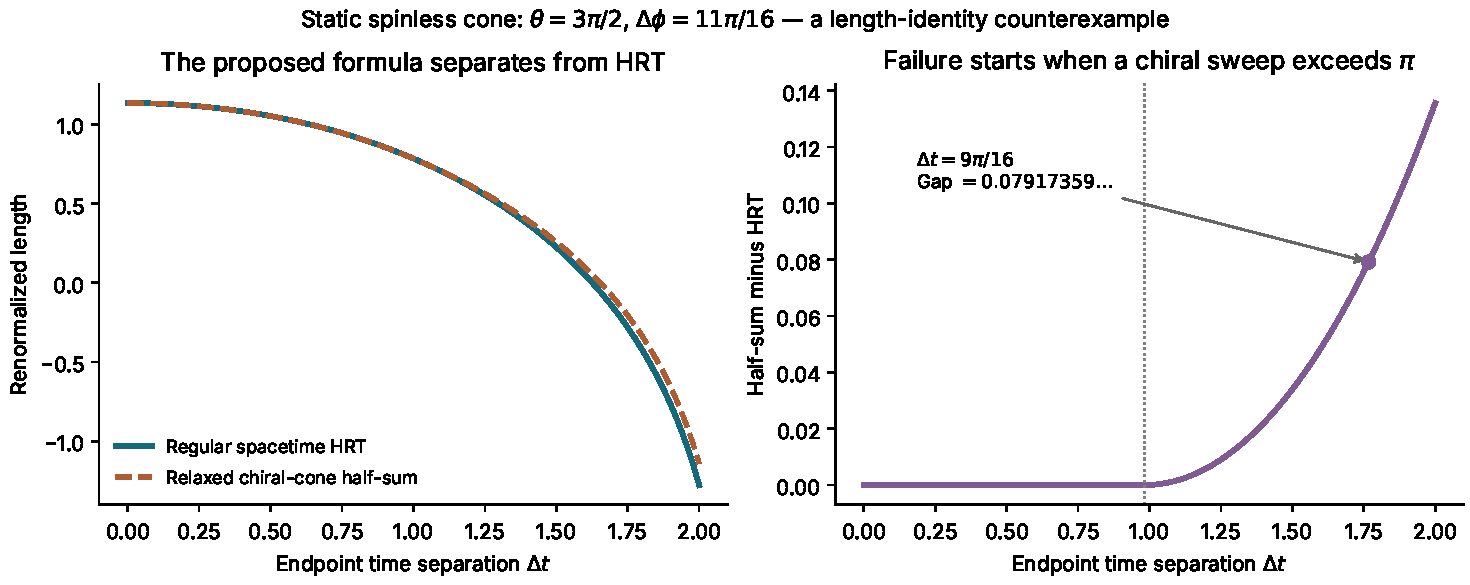
\includegraphics[width=1\textwidth,height=0.72\textheight,keepaspectratio]{particles/figures/tilted_cone_counterexample.pdf}
\caption{The two formulas agree until the direct chiral sweep reaches
pi, then separate. This is a counterexample to the chiral identity, not
to an entropy inequality.}
\end{figure}

\clearpage

\Needspace{8\baselineskip}
\section{Why filled-isotopy Crofton
fails}\label{why-filled-isotopy-crofton-fails}

Research audit, 28 November 2026. This note addresses the proposed
point-particle extension of \texttt{PROOFS.md} Sections 1--4 and
\texttt{fullcone/FULLCONE.md}.

\Needspace{6\baselineskip}
\subsection{1. Decisive result: filling the cones in the intersection
classes fails at every positive-mass
angle}\label{decisive-result-filling-the-cones-in-the-intersection-classes-fails-at-every-positive-mass-angle}

\textbf{Proposition.} For every cone angle \(0<\theta<2\pi\), the
complete hyperbolic cone

\[
C_\theta:\qquad ds^2=dr^2+\sinh^2r\,d\phi^2,
\qquad \phi\in\mathbb R/\theta\mathbb Z
\]

has a globally minimizing regular anchored geodesic \(c\), and an open
positive-Liouville-measure family of regular embedded complete geodesics
\(g\), for which

\[
\#(g\cap c)=2,
\qquad i_{\mathrm{filled}}([g],[c])=0.
\]

Neither curve hits the cone. Thus deleting the measure-zero set of
cone-hitting geodesics does not repair the identity \texttt{(B0)} in the
repository. Restricting the angle below \(\pi\) does not repair that
identity when intersection classes are taken on the filled surface.

\Needspace{5\baselineskip}
\subsubsection{Explicit construction}\label{explicit-construction}

Choose

\[
\max(0,\theta-\pi)<\beta<\theta/2,
\qquad
0<\eta<\min\{\beta/2,(\pi-\theta+\beta)/2,2\pi-\theta\}.
\]

Let \(c\) have ideal endpoints at angular coordinates \(0,\beta\), using
the short angular sector. Let \(g\) have physical ideal endpoints
\(\eta,\beta-\eta\), but use the lift whose angular interval is

\[
(\beta-\eta,\theta+\eta).
\]

Its angular sweep is

\[
\delta_g=\theta-\beta+2\eta<\pi,
\qquad \delta_g<\theta.
\]

It is therefore a regular embedded complete geodesic. A complete regular
hyperbolic geodesic spanning an angular interval \((a,b)\) of length
\(\delta=b-a<\pi\) has polar equation

\[
\tanh r\cos(\phi-\mu)=\cos(\delta/2),
\qquad \mu=(a+b)/2.
\tag{1}
\]

The first intersection of \(g\) with the lift of \(c\) in \((0,\beta)\)
lies in \((\beta-\eta,\beta)\). The second intersection, with the next
lift of \(c\), lies in \((\theta,\theta+\eta)\). At each overlap, the
corresponding developed geodesic endpoint pairs alternate, so there is
exactly one transverse intersection. No further lifts of \(c\) have an
angular interval meeting that of \(g\).

After projection to the cone, the two intersections remain distinct:
their angular coordinates lie respectively in \((\beta-\eta,\beta)\) and
\((0,\eta)\). Both physical endpoints of \(g\) lie in the same boundary
cap cut off by \(c\). On the filled topological disk, \(g\) can be moved
entirely into that cap, disjoint from \(c\). Hence its filled geometric
intersection number is zero.

The cut \(c\) is globally minimizing. Any of its subsegments has angular
difference smaller than \(\beta<\theta/2\). Among lifts of its
endpoints, this is the smallest absolute angular difference. For fixed
radial endpoints the hyperbolic distance is increasing with angular
difference on \([0,\pi]\), by

\[
\cosh d=\cosh r_1\cosh r_2-\sinh r_1\sinh r_2\cos\Delta\phi.
\]

A filled-space minimizing path cannot pass through a cone of angle below
\(2\pi\): one of the two sectors at the tip has angle below \(\pi\), and
smoothing into that sector shortens it. Thus no omitted cone-hitting
path is shorter. The complete anchored version follows by the cutoff
limit.

All endpoint inequalities above are strict. The two intersections
persist under independent small perturbations of the endpoints of \(g\).
In a developed endpoint chart the Liouville density is positive,

\[
d\mu=\frac{da\,db}{4\sin^2((b-a)/2)}.
\]

Consequently the failure occurs on an open set of strictly positive
measure, in a compact part of the cut. It is not a cutoff-end artifact.

\Needspace{5\baselineskip}
\subsubsection{Concrete angles on both sides of the proposed
threshold}\label{concrete-angles-on-both-sides-of-the-proposed-threshold}

\begin{longtable}[]{@{}
  >{\raggedright\arraybackslash}p{(\columnwidth - 6\tabcolsep) * \real{0.2500}}
  >{\raggedright\arraybackslash}p{(\columnwidth - 6\tabcolsep) * \real{0.2500}}
  >{\raggedright\arraybackslash}p{(\columnwidth - 6\tabcolsep) * \real{0.2500}}
  >{\raggedright\arraybackslash}p{(\columnwidth - 6\tabcolsep) * \real{0.2500}}@{}}
\toprule\noalign{}
\begin{minipage}[b]{\linewidth}\raggedright
Cone angle
\end{minipage} & \begin{minipage}[b]{\linewidth}\raggedright
Cut sweep
\end{minipage} & \begin{minipage}[b]{\linewidth}\raggedright
Endpoint displacement
\end{minipage} & \begin{minipage}[b]{\linewidth}\raggedright
Test-geodesic sweep
\end{minipage} \\
\midrule\noalign{}
\endhead
\bottomrule\noalign{}
\endlastfoot
\(\theta=\pi/2\) & \(\beta=\pi/6\) & \(\eta=\pi/48\) & \(3\pi/8\) \\
\(\theta=3\pi/2\) & \(\beta=5\pi/8\) & \(\eta=\pi/32\) & \(15\pi/16\) \\
\end{longtable}

The companion code verifies the two transverse intersections at high
precision and draws the curves in a topological disk rendering. The
argument itself is analytic and valid for every \(\theta\in(0,2\pi)\).

\Needspace{6\baselineskip}
\subsection{2. Filled homology and punctured isotopy are different
operations}\label{filled-homology-and-punctured-isotopy-are-different-operations}

The physically natural condition that particles are included in the
homology region does \textbf{not} require forgetting the particles when
labeling curve classes.

The consistent alternative is:

\begin{itemize}
\tightlist
\item
  Curves and test classes lie in the regular surface
  \(S^\circ=S\setminus Q\), with isotopies avoiding the particle marks
  \(Q\).
\item
  A homology region is a region of the filled surface \(S\), so it may
  contain any subset of particles.
\item
  A closed cut component bounding a disk in the filled surface may be
  deleted when minimizing. Deleting it can only decrease intersection
  counts with every test class. This deletion is an operation on
  admissible cuts; it must not be used to identify arbitrary arc classes
  while retaining an ambiguous intersection number.
\end{itemize}

For the construction above,

\[
i_{\mathrm{punctured}}([g],[c])=2.
\]

The apparent bigon contains the cone point and is not an empty bigon in
\(S^\circ\).

\Needspace{5\baselineskip}
\subsubsection{Minimal-position lemma in punctured
classes}\label{minimal-position-lemma-in-punctured-classes}

\textbf{Lemma.} Suppose the curves in question have regular geodesic
representatives, and one is an embedded cut component. Their transverse
intersections realize the geometric intersection number in the punctured
surface (with the usual proper/ideal endpoint control).

\textbf{Proof.} A nonminimal transverse configuration has an empty
bigon, or the corresponding monogon for a removable self-intersection.
An empty bigon in the punctured surface contains no cone point. If its
corner angles are \(\alpha,\beta>0\), Gauss--Bonnet gives

\[
-\operatorname{Area}(B)+(\pi-\alpha)+(\pi-\beta)=2\pi,
\]

which is impossible. Ideal-end versions follow by truncation in the
hyperbolic ends. The same calculation rules out an empty monogon. The
ordinary bigon criterion therefore applies. The conclusion does not
require an angle threshold once regular representatives exist.
\(\square\)

This repairs the \emph{local minimal-position obstruction}, but does not
by itself establish the full geodesic-current/Crofton representation:
one must also justify the appropriate global space and measure of
complete test geodesics, escape/properness where used, and the near-end
renormalization.

\Needspace{6\baselineskip}
\subsection{\texorpdfstring{3. What the angle \(\pi\) actually
controls}{3. What the angle \textbackslash pi actually controls}}\label{what-the-angle-pi-actually-controls}

The threshold controls realization of arbitrary punctured simple classes
by regular geodesics, rather than the filled-topology Crofton identity.

For cone angles strictly below \(\pi\), both angular sectors at a
cone-hitting limiting curve have angle below \(\pi\). One can shorten
while staying on whichever side is required by the punctured class. This
is the local reason minimizing sequences cannot collapse into the cone
for essential simple curves. Bonsante--Schlenker prove geodesic
realization of laminations in the marked-point complement.
Tan--Wong--Zhang prove unique regular realizations for essential
nonperipheral simple closed curves and essential normal arcs on compact
cone surfaces; their \(\pi\)-angle addenda explicitly contain doubled
cone-to-cone or boundary-to-cone segments.

For angles above \(\pi\), a simple punctured class can have no regular
geodesic representative. On \(C_\theta\), choose ideal endpoints with

\[
0<\beta<\theta-\pi.
\]

The long-side simple arc class has angular sweep \(\theta-\beta>\pi\).
No regular complete geodesic has this sweep: equation (1) requires a
sweep strictly below \(\pi\). Its infimum is approached by paths through
an arbitrarily small neighborhood of the cone; the limiting two radial
rays pass through the singular point. Smoothing to the other side would
shorten it, but changes the punctured class.

Thus:

\begin{longtable}[]{@{}
  >{\raggedright\arraybackslash}p{(\columnwidth - 4\tabcolsep) * \real{0.3333}}
  >{\raggedright\arraybackslash}p{(\columnwidth - 4\tabcolsep) * \real{0.3333}}
  >{\raggedright\arraybackslash}p{(\columnwidth - 4\tabcolsep) * \real{0.3333}}@{}}
\toprule\noalign{}
\begin{minipage}[b]{\linewidth}\raggedright
Claim
\end{minipage} & \begin{minipage}[b]{\linewidth}\raggedright
\(0<\theta<\pi\)
\end{minipage} & \begin{minipage}[b]{\linewidth}\raggedright
\(\pi<\theta<2\pi\)
\end{minipage} \\
\midrule\noalign{}
\endhead
\bottomrule\noalign{}
\endlastfoot
Filled-space minimizing path avoids cone & Yes & Yes \\
Filled-class geodesic/Crofton minimal position for all test geodesics &
\textbf{False} & \textbf{False} \\
Regular geodesics are in punctured minimal position & Yes & Yes \\
Every essential simple punctured class has a regular geodesic &
Available under the cited hypotheses & False in general \\
\end{longtable}

\Needspace{6\baselineskip}
\subsection{4. The topological contraction lemma with particle
marks}\label{the-topological-contraction-lemma-with-particle-marks}

Lemma A can be adapted with punctured isotopy and filled homology.
Choose an auxiliary smooth negatively curved reference surface with
additional funnel ends representing the particles. These auxiliary ends
have \textbf{free colors}: no party boundary condition is imposed there.
Physical asymptotic ends and their marked endpoints retain their
original party assignment.

Place the input cuts in geodesic position for the reference metric. The
cell-coloring and contraction-map construction is unchanged. Near an
auxiliary particle end, the output color is whatever the contraction map
assigns to the input cell color; this is allowed because the filled
homology region may include or exclude that particle. No output cut must
terminate at a particle. Any resulting closed component which is
null-homotopic after filling the particles may be removed. This
decreases every punctured intersection count and preserves the required
physical boundary trace.

The proof of the contraction inequality then uses punctured intersection
numbers in the auxiliary negatively curved surface, exactly as in the
repository proof. This is a topological lemma. Its successful extension
does not establish the physical HRT formula or the required positive
measure in each chiral cone metric.

\Needspace{6\baselineskip}
\subsection{5. A direct disk
alternative}\label{a-direct-disk-alternative}

For a single Riemannian cone disk, globally minimizing
boundary-to-boundary distances satisfy both cyclic crossing inequalities
by ordinary cut-and-paste. If \(a,b,c,d\) occur in cyclic order, the two
minimizing paths \(a\!c\) and \(b\!d\) must intersect. Reconnecting
their segments gives

\[
D(a,c)+D(b,d)\ge D(a,d)+D(b,c),
\qquad
D(a,c)+D(b,d)\ge D(a,b)+D(c,d).
\]

No curvature sign enters this argument. Positive sums of such
boundary-distance matrices retain the inequalities and admit the finite
positive graph construction already proved in
\texttt{strips/FINITE\_\allowbreak GRAPH.md}, after the same explicit endpoint
completion.

This is a genuine mathematical bypass of the cone Crofton obstruction on
a disk. The physical premise must still be established: HRT for the
spacetime must equal the noncrossing matching minimum built from those
interval data. One must not replace a particle-marked common class by
independent left/right minima without proof.

\Needspace{6\baselineskip}
\subsection{6. Branched CAT(-1) cover: promising, not completed
here}\label{branched-cat-1-cover-promising-not-completed-here}

For finitely many cone metrics on the same marked bordered surface,
choose an integer \(q\) with \(q\theta_{j,p}\ge2\pi\) at every particle
and in every metric. A finite cyclic branched cover can have
ramification \(q\) at all particle points; boundary monodromy absorbs
the relation because the surface has boundary. The pullback metrics have
nonpositive cone curvature and are locally CAT(-1).

Liouville-current length identities for nonpositively curved cone
metrics are available in the literature (see Constantine below). A
possible proof would build a deck-equivariant graph upstairs and descend
an invariant minimum cut. This requires a separate argument; it is not
proved merely by lifting the metrics.

One useful local lemma is available. Suppose a descended finite frontier
meets a particle. Choose a pairing of adjacent incident rays bounding a
sector of angle below \(\pi\) in one metric; such a sector exists
because the total angle is below \(2\pi\). Resolve that pairing at a
fixed small radius in this metric to obtain a strict length reduction.
In every other metric, implement the same topological pairing in
arbitrarily small collars; the excess over the cone-hitting broken path
tends to zero. Thus the weighted sum strictly decreases. No side needs
to have angle below \(\pi\) in \emph{all} metrics. Applying this lemma
to an invariant graph minimum requires proving that its descended finite
frontier and metricwise representatives carry the same local pairing
data.

\Needspace{6\baselineskip}
\subsection{Primary sources}\label{primary-sources}

\begin{enumerate}
\def\labelenumi{\arabic{enumi}.}
\tightlist
\item
  F. Bonsante and J.-M. Schlenker, \emph{AdS manifolds with particles
  and earthquakes on singular surfaces},
  \href{https://arxiv.org/abs/math/0609116}{arXiv:math/0609116}, Lemma
  1.1 / Lemma 2.2 and Remark 2.1. Their topology keeps the particle
  marks in the isotopy problem. The spacetime particles in that paper
  are spinless.
\item
  S. P. Tan, Y. L. Wong and Y. Zhang, \emph{Generalizations of McShane's
  identity to hyperbolic cone-surfaces},
  \href{https://arxiv.org/abs/math/0404226}{arXiv:math/0404226}, Theorem
  4.1 and Addendum 4.2. The boundary-arc theorem there uses normal arcs
  to geometric boundary, so its application to fixed ideal endpoints
  needs the usual end-extension argument.
\item
  D. Constantine, \emph{Marked length spectrum rigidity in nonpositive
  curvature with singularities},
  \href{https://dconstantine.faculty.wesleyan.edu/files/2019/08/MLSnonpos.pdf}{author
  PDF}. Relevant to the proposed branched-cover repair; its hypotheses
  and the extension to asymptotic ends must be checked in a complete
  proof.
\end{enumerate}

The all-angle counterexample and the direct elementary arguments above
are derived in this note. They do not claim a counterexample to the
holographic entropy cone: they disprove the proposed filled-topology
intermediate identity.

\begin{figure}
\centering
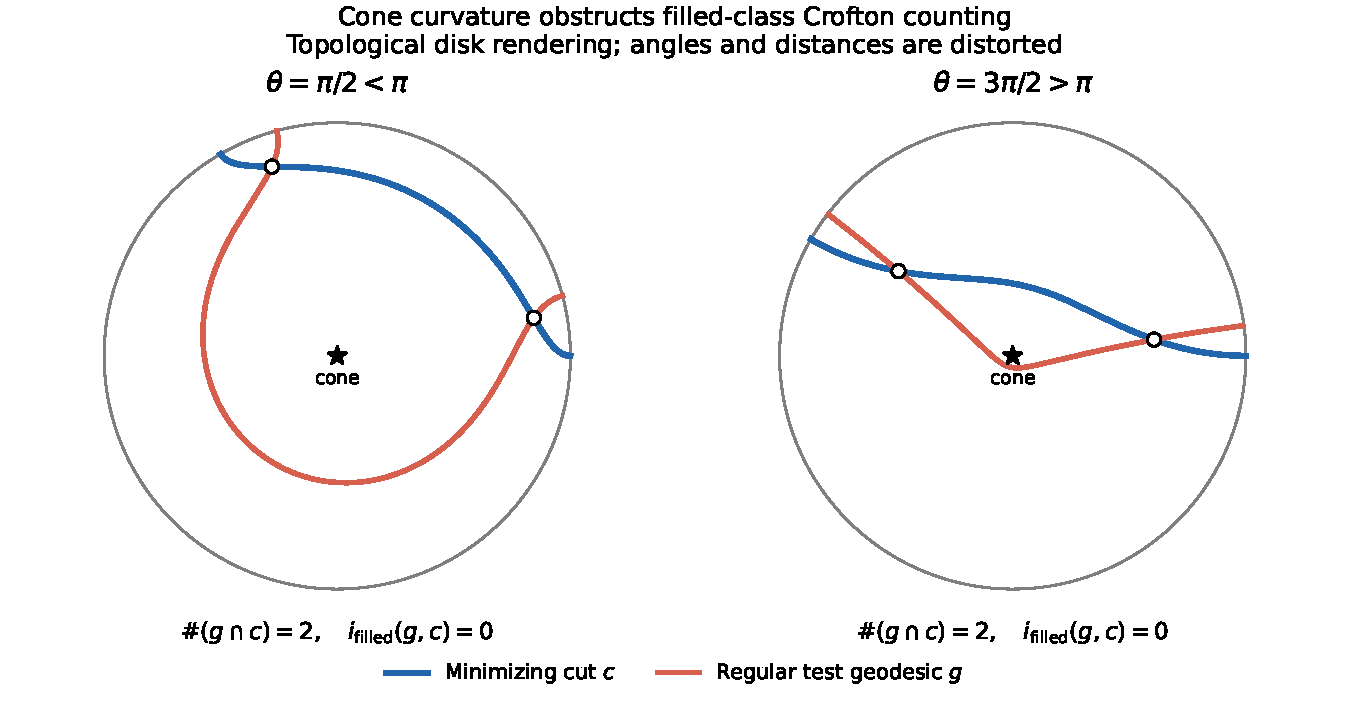
\includegraphics[width=0.85\textwidth,height=0.72\textheight,keepaspectratio]{particles/figures/cone_bigon.pdf}
\caption{An open family of regular test geodesics crosses a minimizing
cut twice although the filled-disk intersection number is zero. The
rendering is topological.}
\end{figure}

\clearpage

\Needspace{8\baselineskip}
\section{Local common-side rounding}\label{local-common-side-rounding}

Research proposition, 28 November 2026. This is a local weighted-length
statement. It does not by itself prove compactness or global attainment
of a minimum over marked curve classes.

\Needspace{6\baselineskip}
\subsection{Proposition}\label{proposition}

Let \texttt{h\_\allowbreak 1,...,h\_\allowbreak m} be cone metrics at a commonly marked point
\texttt{q}, with total angles
\texttt{0\textless{}theta\_\allowbreak j\textless{}2\ pi}, and let
\texttt{w\_\allowbreak j\textgreater{}0}.

Suppose, in each metric, a finite frontier is made of
\texttt{2r\textgreater{}=2} regular radial geodesic germs ending at
\texttt{q}. The germs are indexed in the same cyclic order in every
metric, and the sectors have the same alternating binary region colors.
Assume distinct germs, or a limiting configuration admitting arbitrarily
small compatible disjoint perturbations at arbitrarily small extra
length.

Then there is a \textbf{single common topological resolution} of the
frontier, avoiding \texttt{q}, whose metricwise representatives have
weighted total length strictly less than that of the cone-hitting
frontiers. Outside an arbitrarily prescribed cone chart the
representatives are unchanged. Their physical boundary trace is
unchanged, with \texttt{q} filled for homology.

The resolution need not preserve a preassigned punctured isotopy class:
it selects one of the particle-side choices. It is an admissible
competitor when minimizing over all particle-marked cut classes with
filled homology.

\Needspace{6\baselineskip}
\subsection{Proof}\label{proof-1}

Fix one metric \texttt{h\_\allowbreak j0}. The \texttt{2r} adjacent sector angles
add up to \texttt{theta\_\allowbreak j0\textless{}2\ pi}, so at least one adjacent
sector has angle \texttt{alpha\textless{}pi}. Choose its bounding pair
of germs.

There are two canonical noncrossing resolutions of an alternating binary
star: include a small disk around the point in the selected region and
pair the rays around the complementary sectors, or exclude the disk and
pair around the selected sectors. Choose the resolution containing the
chosen adjacent pair. This fixes a common pairing in every metric,
without asking the same sector to be short in those other metrics.

At equal small radius \texttt{rho} on the chosen two germs of metric
\texttt{j0}, their original broken path through the cone has length
\texttt{2\ rho}. The hyperbolic chord within the sector has length

\[
d_\alpha(\rho)=\operatorname{arcosh}
\big(\cosh^2\rho-\sinh^2\rho\cos\alpha\big)
<2\rho.
\]

Its strict saving is

\[
\delta=2\rho-d_\alpha(\rho)>0,
\qquad
d_\alpha(\rho)=2\rho\sin(\alpha/2)+O(\rho^3).
\]

All other pairs in this metric can be rounded in their prescribed
sectors at radius \texttt{epsilon}, with added length bounded by a
constant times \texttt{epsilon}. Such a connector follows each radial
germ to radius \texttt{epsilon}, runs along the radius-\texttt{epsilon}
circle through the prescribed sector, and returns along the other germ.
Its length excess over the cone-hitting path tends to zero. The same
construction applies to \textbf{all} pairs in every other metric,
regardless of whether the chosen sector there has angle above or below
\texttt{pi}.

The prescribed pairings involve disjoint adjacent sectors, so the local
connectors can be made embedded and mutually disjoint. The chosen chord
lies in its own sector. The same pairing gives the same particle-marked
topological resolution in all metrics.

Choose the remaining rounding radii sufficiently small that the sum of
all weighted excesses is less than \texttt{w\_\allowbreak j0\ delta/2}. The total
weighted length then decreases by at least \texttt{w\_\allowbreak j0\ delta/2}.
Slight smoothing preserves the strict inequality. Including or excluding
the small disk changes only the particle's region color, so filled
homology and all physical boundary labels are preserved. \texttt{QED}

\Needspace{6\baselineskip}
\subsection{Exact limitation}\label{exact-limitation}

This proves that a finite cone-hitting common frontier with compatible
local star data cannot be a global minimum when both particle-side
resolutions are admissible. It does not prove that a minimizing sequence
in different punctured classes converges to such a common finite star,
nor that two independently tightened chiral representatives have
compatible local pairing data. Those are precisely the additional
statements needed before using this proposition in a general all-angle
existence theorem or a branched-cover descent.

\Needspace{6\baselineskip}
\subsection{Why arbitrary marked pairs need not have joint regular
attainment}\label{why-arbitrary-marked-pairs-need-not-have-joint-regular-attainment}

There is an elementary counterexample to the unrestricted statement that
a common-class minimum for two cone metrics must have regular geodesic
representatives in both metrics.

Take two copies of a hyperbolic cone of total angle
\texttt{theta=3\ pi/2}, with commonly marked interval endpoints whose
angular separations are

\[
\beta_L=5\pi/4,\qquad \beta_R=\pi/8.
\]

The common punctured disk has exactly two embedded anchored arc classes.
Their sector sweeps in the two metrics are

\begin{longtable}[]{@{}lrr@{}}
\toprule\noalign{}
Common class & Left sweep & Right sweep \\
\midrule\noalign{}
\endhead
\bottomrule\noalign{}
\endlastfoot
First side & \texttt{5\ pi/4} & \texttt{pi/8} \\
Other side & \texttt{pi/4} & \texttt{11\ pi/8} \\
\end{longtable}

For an anchored class with sweep \texttt{delta}, radial cutoff
\texttt{r=R} gives

\[
L^{\rm ren}(\delta)=
\begin{cases}
2\log\sin(\delta/2),&0<\delta<\pi,\\
0,&\delta\ge\pi.
\end{cases}
\]

The first line follows from the hyperbolic distance formula after
subtracting \texttt{2R}. In the second line, the infimum is the broken
radial path through the cone: regular representatives can approach it
arbitrarily closely, but a regular complete geodesic cannot sweep an
angle at least \texttt{pi} in the developed cone chart.

Thus the first common class has a cone-hitting left infimum and a
regular right geodesic; the second class has the reverse behavior. No
class has regular geodesic representatives in both metrics. A positive
weighted common-class infimum exists as a number, but it is not jointly
regularly attained. Particle-peripheral closed components cannot help
because they are removable with filled homology.

This is a counterexample for \textbf{arbitrary pairs of marked cone
metrics}. It does not establish that these markings arise from a
globally admissible particle spacetime with the proposed
HRT/chiral-length identification. Its role is to show that an
unrestricted mathematical joint-regular-attainment claim cannot be
inserted into that identification without additional spacetime input.

\clearpage

\Needspace{8\baselineskip}
\section{Exact collision kernel: positivity and the graph
theorem}\label{exact-collision-kernel-positivity-and-the-graph-theorem}

Research result, 28 November 2026. The single-interval input is the
explicit two-massless-particle black-hole formation calculation of
Aref'eva, Khramtsov, and Tikhanovskaya, arXiv:1706.07390v3, equations
(3.40), (4.5), and (4.6). The result below proves an all-time statement
about that interval kernel and its noncrossing-matching functional.
Identifying this functional with physical HRT for every union still
requires simultaneous admissibility.

\Needspace{6\baselineskip}
\subsection{1. The exact kernel}\label{the-exact-kernel}

The boundary circle has circumference \(2\pi\). The injection points are
\(0,\pi\), the final nonrotating BTZ radius is \(R>0\), and \(t\ge0\) is
the BTZ rest-frame boundary time. This coordinate is not global
collision time: the particles have \(r(t)=R\coth(Rt)\) and approach the
final horizon as \(t\to\infty\). The original global-coordinate
collision is not a finite event on this time axis.

For endpoints whose shorter arc crosses the injection at zero, choose

\[
-\pi<a<0<b<\pi,\qquad b-a\le\pi,
\]

and define

\[
X=e^{Ra},\quad Y=e^{Rb},\quad Z=e^{Rt},\quad
H=\frac{\pi R}{2},\quad E=\coth H.
\]

Thus \(0<X<1<Y\), \(Z\ge1\), and \(d=\tfrac12\log(Y/X)\le H\). Omit a
common endpoint term for the moment. The direct and crossing lengths are

\[
D_{\mathrm d}=\log\frac{(Y-X)^2}{XY},
\qquad
D_{\mathrm c}=\log\frac{F_1F_2}{XYZ^2},
\tag{1}
\]

where

\[
\begin{aligned}
F_1&=E(X-Z)(Y-Z)+Z(Y-X),\\
F_2&=E(XZ-1)(YZ-1)+Z(Y-X).
\end{aligned}
\tag{2}
\]

Expansion of (2) gives exactly the logarithm argument in the published
crossing formula (3.40); the companion script verifies this identity
symbolically. The published interval kernel is

\[
D_t(a,b)=\min\{D_{\mathrm d},D_{\mathrm c}\}
 +2\log(1/\epsilon).
\tag{3}
\]

If the shorter arc crosses no injection point, use the direct branch. If
it crosses \(\pi\), translate the crossing chart by \(\pi\). The circle
kernel is symmetric under complementation, so for arcs longer than
\(\pi\) use their shorter complement. The endpoint cutoff in (3) is our
consistent dimensionless prescription; no squared-cutoff convention from
the source is imported.

\Needspace{6\baselineskip}
\subsection{2. Positive factors and endpoint
monotonicity}\label{positive-factors-and-endpoint-monotonicity}

Put \(r_i=F_i/[Z(Y-X)]\). Completing the two elementary
arithmetic-geometric mean bounds gives

\[
\begin{aligned}
r_1&=1+E\frac{Z+XY/Z-X-Y}{Y-X},\\
r_2&=1+E\frac{XYZ+1/Z-X-Y}{Y-X},
\end{aligned}
\]

and hence, for either factor,

\[
r_i\ge1-E\frac{\sqrt Y-\sqrt X}{\sqrt Y+\sqrt X}
 =1-E\tanh(d/2)
 \ge\frac1{1+\cosh H}>0.
\tag{4}
\]

There is therefore no hidden logarithm-sign or branch ambiguity. Let
\(h=D_{\mathrm c}-D_{\mathrm d}=\log(r_1r_2)\). Exact differentiation
gives

\[
\begin{array}{ll}
\displaystyle \partial_Xr_1=\frac{E(Y-Z)^2}{Z(Y-X)^2},&
\displaystyle \partial_Yr_1=-\frac{E(X-Z)^2}{Z(Y-X)^2},\\[6pt]
\displaystyle \partial_Xr_2=\frac{E(YZ-1)^2}{Z(Y-X)^2},&
\displaystyle \partial_Yr_2=-\frac{E(XZ-1)^2}{Z(Y-X)^2}.
\end{array}
\tag{5}
\]

Consequently

\[
h_a\ge0,\qquad h_b\le0.
\tag{6}
\]

These signs hold throughout the physical shortest-arc patch, including
times after equilibration. They are the ingredient needed to control the
minimum of the two branches; positivity of the separate branches alone
would not suffice.

\Needspace{6\baselineskip}
\subsection{3. Positivity through every branch
change}\label{positivity-through-every-branch-change}

The determinant of each bilinear polynomial is particularly simple:

\[
F_i\partial_X\partial_YF_i
 -(\partial_XF_i)(\partial_YF_i)=Z^2.
\tag{7}
\]

It follows that

\[
\partial_a\partial_b D_{\mathrm c}
 =R^2XY Z^2(F_1^{-2}+F_2^{-2})>0,
\qquad
\partial_a\partial_b D_{\mathrm d}
 =\frac{2R^2XY}{(Y-X)^2}>0.
\tag{8}
\]

For a regular switch curve, the additional mixed measure is formally
\(-\delta(h)h_ah_b\), which is nonnegative by (6). The following
argument also covers tangencies and singular switch loci. Choose smooth
concave functions \(f_\eta\to\min(0,\cdot)\), with \(0\le f_\eta'\le1\)
and \(f_\eta''\le0\). Then

\[
\begin{aligned}
\partial_a\partial_b\bigl(D_{\mathrm d}+f_\eta(h)\bigr)
={}&(1-f_\eta')\,\partial_a\partial_bD_{\mathrm d}
 +f_\eta'\,\partial_a\partial_bD_{\mathrm c}\\
 &+f_\eta''h_ah_b\ \ge0.
\end{aligned}
\tag{9}
\]

Taking the distributional limit proves positivity without a regularity
assumption on the transition locus.

\Needspace{5\baselineskip}
\subsubsection{Injection-point seams}\label{injection-point-seams}

At \(a=0\), \(t=0\), both factors in (4) equal one, so the crossing and
direct values agree. Their tangential \(b\)-derivatives agree as well.
For \(t>0\), the direct branch is selected in a neighborhood of this
seam. One way to see this last fact is to rewrite the crossing argument
as

\[
4\left[Q^2+\sinh^2m(E^2-P^2)\right],\quad
P=\sinh d-E\cosh d,\quad Q=E\cosh(Rt)+\cosh m\,P,
\tag{10}
\]

where \(m=R(a+b)/2\), \(|m|\le d\). Here \(P<0\) and

\[
Q\ge \sinh d\,[\cosh d-E\sinh d]\ge0.
\]

Increasing \(t\) strictly increases (10) away from the degenerate
boundary point, while the direct length is fixed. At the seam their
initial values are equal. The same argument applies at \(b=0\) and at
the other injection. Thus patching across these seams creates no
negative mixed measure.

\Needspace{5\baselineskip}
\subsubsection{Antipodal seams}\label{antipodal-seams}

At \(b-a=\pi\), changing to the complementary injection chart sends
\((a,b)\mapsto(b-\pi,a+\pi)\). It leaves \(m\) fixed and sends
\(d\mapsto2H-d\). At \(d=H\),

\[
P=-\frac1{\sinh H},\qquad P'=\cosh H-E\sinh H=0.
\]

Equation (10) therefore has \(\partial_dD_{\mathrm c}=0\) there. The
direct branch has \(\partial_dD_{\mathrm d}=2\coth H>0\). After
reflection about \(d=H\), any derivative jump is downward in the
separation coordinate. Since
\(\partial_a\partial_b=(R^2/4)(\partial_m^2-\partial_d^2)\), its mixed
measure is nonnegative. This includes the case when the two branches tie
at the antipodal seam.

\Needspace{6\baselineskip}
\subsection{4. The all-time theorem and its graph
corollary}\label{the-all-time-theorem-and-its-graph-corollary}

\textbf{Theorem K.} For every \(R>0\) and \(t\ge0\), the symmetric
equal-time circle interval kernel (3), patched as above, has a
nonnegative distributional kinematic measure away from coincident
endpoints:

\[
\boxed{\partial_a\partial_b D_t\ge0.}
\tag{11}
\]

Equivalently, every cyclically ordered quadruple obeys

\[
D_t(a,c)+D_t(b,d)\ge D_t(a,d)+D_t(b,c).
\tag{12}
\]

The proof uses the exact published kernel and elementary algebra. It
does not invoke maximin, the null energy condition, or a guessed
Lorentzian triangle inequality. It is a theorem about the kernel; the
geometric derivation of that kernel remains the stated input.

Fix finitely many distinct boundary endpoints \(x_0,\ldots,x_{m-1}\),
ordered cyclically, and set \(D_{ii}=0\). For a sufficiently small fixed
cutoff, all discrete weights

\[
w_{ij}=\frac12\left[D_{ij}+D_{i+1,j+1}-D_{i,j+1}-D_{i+1,j}\right]
\tag{13}
\]

are nonnegative, with indices interpreted cyclically. Nonadjacent
weights are rectangle integrals of (11); adjacent weights have a
positive endpoint divergence, so sufficiently small cutoff makes the
finite set nonnegative. They reconstruct every interval exactly by
telescoping:

\[
D_{ab}=\sum_{i\in[a,b)}\sum_{j\notin[a,b)}w_{ij}.
\tag{14}
\]

Apply the finite disk chord-arrangement theorem from the standing
\texttt{strips/FINITE\_\allowbreak GRAPH.md} (or the corresponding disk full-cone
theorem). The noncrossing-matching functional

\[
F_t(A)=\min_{\Pi\in\mathrm{NC}(\partial A)}
          \sum_{\{p,q\}\in\Pi}D_t(p,q)
\tag{15}
\]

has one finite nonnegative-capacity graph representing all unions.
Consequently, for every number of parties and every time,

\[
\boxed{\mathbf F_t\in\mathcal C_N^{\mathrm{RT}}.}
\tag{16}
\]

This statement is exact for the defined functional. The arrangement
graph is essential: replacing it by the bare graph of Bell edges between
boundary atoms gives different disconnected-region entropies.

\Needspace{6\baselineskip}
\subsection{5. Precisely what is still needed for physical collision
HRT}\label{precisely-what-is-still-needed-for-physical-collision-hrt}

Every actual HRT cut on a filled-disk homology slice induces a
noncrossing endpoint matching. Its component costs are no smaller than
the globally least single-interval branch costs, provided that the
published interval list exhausts regular admissible component geodesics.
This yields a lower bound by (15). The reverse direction is the missing
statement:

\begin{quote}
A minimizing matching in (15) admits choices of its direct/crossing
geodesic representatives that form one embedded acausal multicurve and
lie on one homology Cauchy slice of the two-particle spacetime.
\end{quote}

Endpoint noncrossing by itself does not prove this Lorentzian assertion.
Cone smoothing and finite-group quotient descent do not prove it either.
Once this geometric lemma is supplied, (16) immediately becomes the
desired arbitrary-party black-hole-formation theorem for this specific
model. Until then, (16) and the numerical outputs must be labelled as
matching functional results, not an unconditional all-union HRT theorem.

The independent geometric audit \texttt{COLLISION\_\allowbreak ADMISSIBILITY.md}
supplies further information about actual branch existence and the
obstruction to a direct vacuum invisible-domain embedding.

\Needspace{6\baselineskip}
\subsection{6. Reproducible numerical
audit}\label{reproducible-numerical-audit}

Run:

\begin{verbatim}
python code/bilocal_collision.py \
  --facets data/facets_n5_all372.json \
  --output data/collision
\end{verbatim}

The computation uses eight distinct ten-endpoint arrangements, three
values \(R=0.5,1,2\), 81 times in \([0,2]\), and 3, 4, or 5 nonempty
parties. For fewer than five parties, the unused parties are empty;
evaluation of all 372 five-party facets therefore also includes the
induced lower-party inequalities. The 372 facet vectors are the complete
five-party catalogue associated with Hernandez-Cuenca, arXiv:1903.09148,
with source URL recorded in the input JSON.

Results:

\begin{itemize}
\tightlist
\item
  5,832 matching entropy vectors; 2,169,504 facet evaluations.
\item
  Minimum residual: \(-1.4211\times10^{-13}\), consistent with
  arithmetic error at exact saturation; the stated acceptance tolerance
  is \(10^{-10}\).
\item
  Minimum discrete kinematic weight: \(2.74628\times10^{-4}>0\).
\item
  Maximum reconstruction error in (14): \(2.8422\times10^{-14}\).
\item
  Exact symbolic checks of (1), (5), and (7) all pass.
\item
  Symmetric-interval saturation at \(t=(b-a)/2\) agrees within
  \(1.78\times10^{-15}\).
\end{itemize}

The samples check the implementation. The all-time cone statement for
the matching functional follows from Sections 2--4, not from time
sampling. The figure labels its multiparty panels accordingly and does
not mark a fictional finite collision time on the BTZ time axis.

\Needspace{6\baselineskip}
\subsection{Primary references}\label{primary-references-1}

\begin{itemize}
\tightlist
\item
  I. Ya. Aref'eva, M. A. Khramtsov, M. D. Tikhanovskaya,
  \emph{Thermalization after holographic bilocal quench}, JHEP 09 (2017)
  115, \url{https://arxiv.org/abs/1706.07390}.
\item
  S. Hernandez-Cuenca, \emph{The Holographic Entropy Cone for Five
  Regions}, Phys. Rev.~D 100 (2019) 026004,
  \url{https://arxiv.org/abs/1903.09148}.
\item
  H.-J. Matschull, \emph{Black Hole Creation in 2+1 Dimensions}, Class.
  Quantum Grav. 16 (1999) 1069,
  \url{https://arxiv.org/abs/gr-qc/9809087}.
\end{itemize}

The algebraic factorization, switch-positivity proof, and all-party
matching corollary are deductions made in this research run; no claim of
literature priority is made without a separate exhaustive novelty
review.

\begin{figure}
\centering
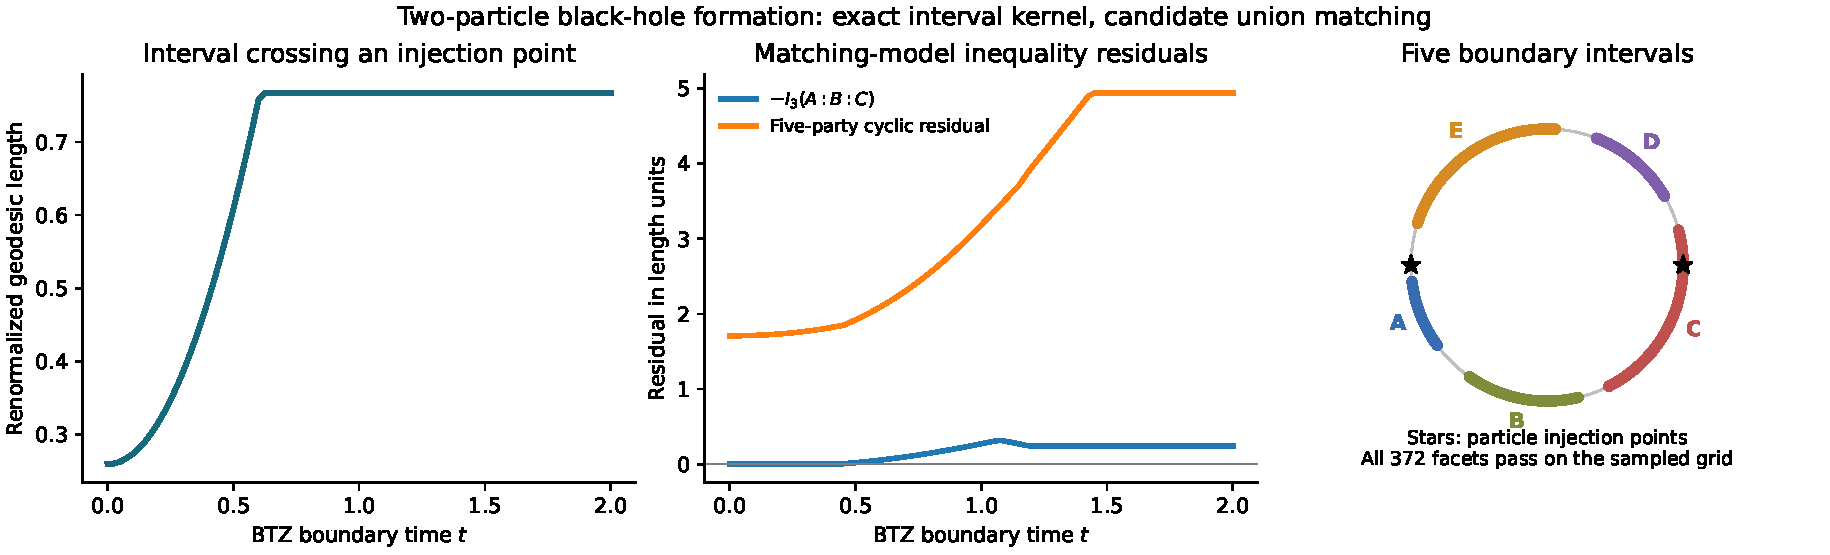
\includegraphics[width=1\textwidth,height=0.72\textheight,keepaspectratio]{particles/figures/collision_matching.pdf}
\caption{The published single-interval kernel and its
noncrossing-matching model. The multiparty panels do not independently
establish physical multicurve admissibility.}
\end{figure}

\clearpage

\Needspace{8\baselineskip}
\section{Collision branches and the remaining realization
problem}\label{collision-branches-and-the-remaining-realization-problem}

28 November 2026. Model: Aref'eva--Khramtsov--Tikhanovskaya,
\href{https://arxiv.org/abs/1706.07390}{arXiv:1706.07390v3}, Sections
2.2--3.3. The statements in Sections 1--5 concern individual equal-time
interval branches. They do not establish simultaneous physical
admissibility of an arbitrary multicomponent matching.

\Needspace{6\baselineskip}
\subsection{1. Notation and developed
geodesics}\label{notation-and-developed-geodesics}

Let \(R>0\), \(\mu=\pi R\), \(E=\coth(\mu/2)\). Consider a shortest
boundary arc crossing particle 1,

\[
 -\pi<a<0<b<\pi,\quad b-a\le\pi,
 \quad c=\frac{R(a+b)}2,\quad d=\frac{R(b-a)}2.
\]

Thus \(|c|<d\le\mu/2\). Both endpoints have the same BTZ time \(t\ge0\).
Write \(C=\cosh Rt\), \(S=\sinh Rt\), and use ambient signature
\((-++-)\). A null boundary representative is

\[
 p(x)=(-\cosh Rx,C,\sinh Rx,S).
\]

The particle holonomy is \(u_1=\bigl(\begin{smallmatrix}1&0\\-2E&1
\end{smallmatrix}\bigr)\). Its \(\#\)-action on an ambient vector is

\[
 \begin{aligned}
 x_0'&=x_0+2Ex_2+2E^2(x_0+x_1),\\
 x_1'&=x_1-2Ex_2-2E^2(x_0+x_1),\\
 x_2'&=x_2+2E(x_0+x_1),\qquad x_3'=x_3.
 \end{aligned}
\]

The crossing curve is recovered from the developed geodesic
\(G(p(a),p(b)^\#)\): keep its left segment up to the wedge face, and map
the other segment by the inverse holonomy. This is precisely the image
construction of the source's equations (3.12)--(3.21).

\Needspace{6\baselineskip}
\subsection{2. Direct appearance and crossing disappearance without a
triangle
inequality}\label{direct-appearance-and-crossing-disappearance-without-a-triangle-inequality}

Define

\[
 P(C)=(C-\cosh(c-d))(C-\cosh(c+d)),\qquad
 Q(C)=C\cosh c-\cosh d,
\]

and

\[
 F(C)=E P(C)+\sinh d\,Q(C).
\]

The direct branch crosses the symmetry plane \(x_2=0\). At that point,
\(x_0+x_1\) has the sign of \(Q\). The regular exterior of the wedge at
that plane has \(x_0+x_1\ge0\). Consequently the direct branch first
becomes available at

\[
 C_{\rm cr}=\frac{\cosh d}{\cosh c},\qquad Q(C_{\rm cr})=0.
\]

This is the source's equation (3.30), obtained directly from the cut
faces.

For the crossing branch, set \(u_a=C-\cosh(c-d)\), \(u_b=C-\cosh(c+d)\),
and

\[
 w_a=\sinh(c-d)-Eu_a<0,\qquad
 w_q=\sinh(c+d)+Eu_b>0.
\]

These inequalities hold for \(t\ge0\) and endpoints in the stated half
circles. The left wedge plane is \(w=x_2-E(x_0+x_1)=0\). An unnormalized
intersection point of the image geodesic with it is

\[
 Y=w_q p(a)-w_a p(b)^\#.
\]

A direct calculation gives

\[
 Y_0+Y_1
 =u_a\sinh(c+d)-u_b\sinh(c-d)+2Eu_au_b
 =2F(C).
\]

The proper wedge face lies on the side \(x_0+x_1\le0\); its endpoint on
particle 1 has \(x_0+x_1=x_2=0\). Hence the crossing branch reaches the
particle precisely when

\[
 F(C_o)=0.
\]

At this point its normalized intersection is on the fixed null line
\(X=(-s,s,0,1)\). This criterion comes from the actual geodesic
embedding, not a comparison of plotted lengths.

There is exactly one root \(C_o>1\). To see this, put
\(H=\cosh d-\cosh c>0\). Then

\[
 F(1)=H(EH-\sinh d)<0,
\]

because \(H\le\cosh d-1=\sinh d\tanh(d/2)\) and \(E\tanh(d/2)<1\). The
quadratic \(F\) has positive leading coefficient, so precisely one of
its two roots is above one.

By reflecting the setup assume \(c\ge0\). Let \(m=\cosh(d-c)\),
\(M=\cosh(d+c)\). Then

\[
 m\le C_{\rm cr}\le M,
 \qquad F(C_{\rm cr})=E P(C_{\rm cr})\le0,
 \qquad F(M)=\sinh d\,Q(M)\ge0.
\]

Thus

\[
 \boxed{C_{\rm cr}\le C_o\le M.}
\]

Equality \(C_o=C_{\rm cr}\) occurs for the symmetric interval \(c=0\).
For a strictly asymmetric interval both branch coexistence inequalities
are strict.

\Needspace{6\baselineskip}
\subsection{3. Exact length comparison at both physical
thresholds}\label{exact-length-comparison-at-both-physical-thresholds}

Use compatible radial cutoffs and omit their common additive divergence.
The exponential of the direct renormalized length is

\[
 K_{\rm dir}=4\sinh^2d.
\]

Expanding \(-2\langle p(a),p(b)^\#\rangle\), or equivalently the
source's equation (3.40), gives

\[
 K_{\rm cross}
 =4\left[\sinh^2d+E^2P(C)+2E\sinh d\,Q(C)\right].
\]

At direct appearance,

\[
 K_{\rm cross}(C_{\rm cr})-K_{\rm dir}
 =4E^2P(C_{\rm cr})\le0.
\]

At crossing disappearance, use \(EP=-\sinh d\,Q\) to obtain

\[
 \boxed{K_{\rm cross}(C_o)-K_{\rm dir}
 =4E\sinh d\,Q(C_o)\ge0.}
\]

This proves the comparison claimed in equation (3.39) of the source
without using its purported Lorentzian triangle inequality. A general
triangle inequality for spacelike sides would not justify that step.

Moreover \(K_{\rm cross}\) is strictly increasing for \(C\ge1\):

\[
 \frac{dK_{\rm cross}}{dC}
 =8E\left[E(C-\cosh c\cosh d)+\sinh d\cosh c\right]>0.
\]

For a convenient lower bound at \(C=1\), use \(\cosh c\le\cosh d\) and
\(E\tanh d\le1\); the derivative increases with \(C\). Strictness
follows from \(|c|<d\). Therefore there is exactly one length switch,
and it lies in the interval where both branches are available. The
formal minimum of these two length expressions never selects the branch
before its physical appearance or after its disappearance.

This uses the source's classification of the relevant short-arc branches
and does not independently classify every winding extremal curve. At a
contact threshold, a limiting curve can meet the null particle
worldline. The expressions above remain continuous limiting lengths;
they are not a claim that the curve at the contact instant belongs to a
regular-locus-only candidate space. A prescription restricted to regular
curves must distinguish its infimum from attainment there.

\Needspace{6\baselineskip}
\subsection{4. Independent audit of the positive interval
kernel}\label{independent-audit-of-the-positive-interval-kernel}

Put \(A=e^{Ra}<1<B=e^{Rb}\), \(T=e^{Rt}\). The exact ratio factors are

\[
 R_1=1+\frac{E(A-T)(B-T)}{T(B-A)},\qquad
 R_2=1+\frac{E(AT-1)(BT-1)}{T(B-A)},
\]

with \(L_{\rm cross}-L_{\rm dir}=h=\log R_1+\log R_2\). Both factors are
positive: their common lower bound is \(1-E\tanh(R(b-a)/4)>0\).

The exact endpoint derivatives are

\[
 \begin{array}{ll}
 (R_1)_A=\dfrac{E(B-T)^2}{T(B-A)^2},&
 (R_1)_B=-\dfrac{E(A-T)^2}{T(B-A)^2},\\[6pt]
 (R_2)_A=\dfrac{E(BT-1)^2}{T(B-A)^2},&
 (R_2)_B=-\dfrac{E(AT-1)^2}{T(B-A)^2}.
 \end{array}
\]

Thus \(h_a\ge0\), \(h_b\le0\). Writing the two crossing factors as
bilinear numerators, each logarithm has positive mixed derivative
because the numerator's \(AB\)-determinant is exactly \(T^2\).

For switch regularity, one need not assume a nonsingular \(h=0\) wall.
Let \(f\) be a smooth concave approximation to \(\min(0,h)\), with
\(0\le f'\le1\), \(f''\le0\). Then

\[
 \partial_a\partial_b[L_{\rm dir}+f(h)]
 =(1-f')\partial_a\partial_bL_{\rm dir}
 +f'\partial_a\partial_bL_{\rm cross}
 +f''h_ah_b\ge0.
\]

Distributional convergence proves positivity of the minimum kernel even
at degenerate switch points. Where the switch wall is regular, the extra
term is the positive measure \(-h_ah_b\,\delta(h)\).

The resulting phase ordering is also exact: a nested outer interval
cannot be in the direct phase while its inner interval is in the
crossing phase.

\Needspace{6\baselineskip}
\subsection{5. Why the Fuchsian two-cusp vacuum domain is
insufficient}\label{why-the-fuchsian-two-cusp-vacuum-domain-is-insufficient}

The special symmetric model has diagonal holonomies, so it is natural to
try to embed it into the vacuum domain of a Fuchsian surface with two
cusps and one funnel. This cannot cover the full post-quench boundary.

The parabolic limit point of particle 1 is \(P=(-1,1,0,0)\), at global
time \(-\pi/2\) and angle zero. The physical boundary point at BTZ time
\(t>0\), angle zero, is

\[
 Q=(-1,\cosh Rt,0,\sinh Rt).
\]

It is timelike to \(P\): the global spatial angle is unchanged and
global time has advanced. Equivalently
\(\langle P,Q\rangle=\cosh Rt-1>0\). Since \(P\) belongs to the diagonal
group's limit set, \(Q\) is outside its invisible domain. The smooth
vacuum cusp theorem therefore does not identify the generic post-quench
HRT family.

\Needspace{6\baselineskip}
\subsection{6. Status of simultaneous realization and the Czech--Dong
result}\label{status-of-simultaneous-realization-and-the-czechdong-result}

\href{https://arxiv.org/abs/1905.03787}{Czech--Dong, arXiv:1905.03787},
Section 2.1, organizes HRT phases as nonalternating colorings; Appendix
A uses SSA to show that spatial ordering minimizes the corresponding
sums of interval entropies. It does not prove an acausal-slice
realization lemma for independently chosen interval minimizers in a
singular point-particle geometry. Its known contraction-inequality
result, including all the five-party inequalities, must be credited;
checking those inequalities numerically here is not a first theorem of
their covariant validity.

The actual missing physical implication remains

\[
 \begin{gathered}
 \text{optimal noncrossing matching of the exact interval kernel}\\
 \Downarrow\\
 \text{one embedded extremal multicurve}\\
 \text{on an acausal homology slice}.
 \end{gathered}
\]

SSA and phase ordering alone are algebraic statements and do not prove
that implication. The exact image-geodesic description above reduces it
to a concrete finite wedge/causality problem in this special model,
rather than the unrestricted BBS collision-surgery problem.

\Needspace{6\baselineskip}
\subsection{7. A reflection-restricted route, preserved as an open
proposition}\label{a-reflection-restricted-route-preserved-as-an-open-proposition}

There is extra structure specific to the symmetric collision which is
absent in general BBS collision surgery. The gluing map on each paired
\(W\) or \(V\) face preserves \(x_0,x_1,x_3\) and sends
\(x_2\mapsto-x_2\). The physical spacetime therefore has a spatial
reflection exchanging two copies of a right half-domain. That
half-domain is bounded by three timelike totally geodesic planes with
inward unit spacelike normals

\[
 n_0=(0,0,1,0),\qquad
 n_1=(-E,E,1,0),\qquad
 n_2=(\sinh\mu,0,-\cosh\mu,0).
\]

Its inequalities are \(\langle X,n_j\rangle\ge0\). The folding map
reflects the negative-\(x_2\) half into the positive half. Piecewise it
is a time-orientation-preserving AdS isometry; along identification
faces it is continuous. Hence it sends causal curves to causal curves.
If a proposed multicurve's folded image is acausal in the ambient AdS
patch, its physical image is acausal as well. The converse need not
hold.

For boundary points of the half-circle write
\(p(u)=(-\cosh u,C,\sinh u,S)\), \(0<u<\mu\). The three positive wall
weights are

\[
 w_0=\sinh u,\quad
 w_1=\sinh u+E(C-\cosh u),\quad
 w_2=\sinh(\mu-u).
\]

A reflection-symmetric full geodesic folds to an orthogeodesic from
\(p(u)\) to one of these walls. Its unfolded endpoints are \(p(u)\) and
\(J_jp(u)\), where \(J_jX=X-2\langle X,n_j\rangle n_j\). Its full length
factor is \(4w_j^2\). The minimum wall is therefore

\begin{itemize}
\tightlist
\item
  \(H_0\) for \(u<Rt\),
\item
  \(H_1\) for \(Rt<u<\mu-Rt\),
\item
  \(H_2\) for \(u>\mu-Rt\),
\end{itemize}

when \(Rt<\mu/2\); after that time only the direct \(H_0,H_2\) branches
remain. Equalities are particle-contact limits.

For reflection-invariant boundary labels, the formal positive graph has
an invariant minimum cut by submodularity. An invariant noncrossing
matching cannot contain an asymmetric opposite-half component together
with its reflected distinct component: their endpoints alternate. Thus
opposite-half components in such a matching are individually symmetric,
while same-half components occur in mirror pairs.

This makes a physical theorem for reflection-invariant parties
plausible. Several local acausality comparisons become transparent. For
example, with \(J=J_1\),

\[
 \langle p(u),Jp(v)\rangle
 =\langle p(u),p(v)\rangle-2w_1(u)w_1(v)<0.
\]

Thus the half-boundary arc and its reflected image form compatible
acausal endpoint sets. Ordered orthogeodesics to the same wall are
noncrossing chords of that set. A same-half direct chord whose endpoints
are on the same side of the orthogeodesic's boundary endpoint is
likewise noncrossing and acausal with it in the developed patch.

\textbf{Unfinished proposition.} Complete all mixed-wall comparisons,
including the \(H_1\)--\(H_0,H_2\) pairs and contact limits, and show
that the folded family extends to a slice whose double is a physical
Cauchy homology surface. These steps have not been packaged into a
checked proof here. This section is a research route, not an additional
established collision entropy-cone theorem. For arbitrary,
non-reflection-invariant parties, folding can create extra interleavings
and cannot be assumed to preserve acausality of the selected family.

\clearpage

\Needspace{8\baselineskip}
\section{Cusps and extremal BTZ}\label{cusps-and-extremal-btz}

Research note, 28 November 2026. This note does not modify the
repository's standing proofs.

\Needspace{6\baselineskip}
\subsection{Status}\label{status}

\begin{enumerate}
\def\labelenumi{\arabic{enumi}.}
\tightlist
\item
  \textbf{Proved:} quantitative continuity of the complete finite-party
  entropy vector in the nonextremal-to-extremal BTZ limit, with no
  escape of minimizing cut classes. Consequently the \emph{limiting BTZ
  entropy prescription} lies in the full RT cone.
\item
  \textbf{Proved:} actual HRT for bounded intervals on the
  \textbf{unwrapped extremal BTZ exterior} has the disk
  matching/positive-graph representation, using a direct Poincare patch
  map and the existing disk homology argument. No horizon component or
  maximin theorem is needed.
\item
  \textbf{Proved obstruction:} a genuine hyperbolic-parabolic quotient
  has no invariant bulk geodesic in its peripheral class. Thus the
  extremal horizon cost is not the length of an attained closed extremal
  curve. The compact black-hole result in item 1 must not be relabelled
  as an attained-HRT theorem for every region.
\item
  \textbf{Mathematical extension:} for hyperbolic surfaces with cusps,
  the Crofton/current argument survives after cusp-peripheral
  zero-infimum components are removed, provided the same cusp labels are
  unmarked in every metric. This does not alone establish the spacetime
  Theorem H for mixed hyperbolic-parabolic ends.
\end{enumerate}

The slogan ``cusps are just horoball cutoffs'' misses the difference
between a parabolic translation-length infimum and a realized geodesic
axis.

\Needspace{6\baselineskip}
\subsection{1. The extremal geometry and its
holonomy}\label{the-extremal-geometry-and-its-holonomy}

Set the AdS radius to one. Write

\[
\alpha=\frac{r_+-r_-}{2},\qquad
\beta=\frac{r_++r_-}{2},\qquad \phi\sim\phi+P.
\]

The ordinary nonextremal family has \(\alpha,\beta>0\). Fix \(\beta>0\)
and take \(\alpha\downarrow0\). At the limit \(r_+=r_-=r_0=\beta\).

Caputa--Jejjala--Soltanpanahi, arXiv:1309.7852v2, equation (2.5), give
the exact exterior-to-Poincare map

\[
w_- =\frac{e^{2r_0(\phi-t)}}{2r_0},\qquad
w_+=\phi+t-\frac{r_0}{r^2-r_0^2},\qquad
U=\frac{e^{r_0(\phi-t)}}{\sqrt{r^2-r_0^2}}.
\tag{1}
\]

It takes the exterior \(r>r_0\) to the half-Poincare patch
\(U>0,w_->0\), with

\[
ds^2=\frac{dU^2+dw_+dw_-}{U^2}.
\]

The spatial identification acts as

\[
(w_+,w_-,U)\longmapsto
(w_++P,e^{2r_0P}w_-,e^{r_0P}U).
\tag{2}
\]

One chiral boundary action is a nontrivial translation, hence parabolic;
the other is a dilation, hence hyperbolic. Setting one diagonal
eigenvalue parameter to zero without a compensating conjugation instead
produces an identity factor and describes a different
quotient/near-horizon degeneration. The self-dual near-horizon quotient
must not be identified with (2).

The same source, equations (2.8)--(2.14), explicitly tracks how the
spatial identification changes in the near-horizon limit.

\Needspace{5\baselineskip}
\subsubsection{The massless and ordinary-cusp cases are
different}\label{the-massless-and-ordinary-cusp-cases-are-different}

Taking \textbf{both} \(\alpha,\beta\to0\), with the correct parabolic
normalization in both factors, gives massless BTZ. Its exterior metric
is

\[
ds^2=-r^2dt^2+\frac{dr^2}{r^2}+r^2d\phi^2,
\qquad \phi\sim\phi+P.
\]

At \(t=0\), setting \(y=1/r\) identifies the spatial metric with
\((d\phi^2+dy^2)/y^2\), a parabolic cylinder. The deep end is a cusp,
its peripheral length has infimum zero, and there is no positive-length
horizon/core geodesic. The boundary-arc formula becomes
\(D_{0,0}=\log(|u_nv_n|/(\epsilon_p\epsilon_q))\). The two-parameter
version of (9) is

\[
0\le F_{\alpha,\beta}(A)-F_{0,0}(A)
\le kP^2(\alpha^2+\beta^2)/6+P(\alpha+\beta).
\]

This again proves full-cone membership for the limiting functional.
Calling the result an attained HRT prescription requires specifying
whether a homology region may extend down the infinite cusp. If only
compact homology chains are permitted, a missing core component cannot
silently be replaced by a zero-length curve. Ordinary cusp ends in
non-elementary hyperbolic surfaces are treated separately in Section 6.

\Needspace{6\baselineskip}
\subsection{2. No closed peripheral geodesic in a hyperbolic-parabolic
quotient}\label{no-closed-peripheral-geodesic-in-a-hyperbolic-parabolic-quotient}

Use the matrix model
\(\mathrm{AdS}_3=\{X\in M_2(\mathbb R):\det X=1\}\). The action is
\(T(X)=LXR^{-1}\), with

\[
L=\begin{pmatrix}e^a&0\\0&e^{-a}\end{pmatrix},\qquad
R=\begin{pmatrix}1&s\\0&1\end{pmatrix},\qquad a>0,\ s\ne0.
\]

Its two generalized eigenspaces are

\[
V_+=\operatorname{span}(E_{11},E_{12}),\qquad
V_-=\operatorname{span}(E_{21},E_{22}),
\]

with distinct eigenvalues \(e^a,e^{-a}\). Each restriction is one
nontrivial Jordan block. Every invariant subspace decomposes under the
two spectral projections, since those projections are polynomials in T.

An invariant two-plane W therefore has dimensions \((2,0)\), \((0,2)\),
or \((1,1)\) in these spaces. In the first two cases it is one of the
row planes \(V_\pm\), on which determinant vanishes identically. In the
last case, the only invariant line in each Jordan block is its
eigenline, giving

\[
W=\operatorname{span}(E_{12},E_{22}),
\]

again a rank-one/determinant-zero plane. Thus \textbf{no invariant
two-plane intersects \(\det X=1\)}.

Every AdS geodesic is the intersection with a two-plane through the
origin (including the degenerate-plane description of null geodesics).
It follows that there is no T-invariant bulk geodesic. The same proof
applies to every nonzero power, since it remains hyperbolic-parabolic.

A closed geodesic in a quotient lifts to a geodesic invariant under its
deck transformation. Consequently exact extremal BTZ has no closed
geodesic in the peripheral winding class. In particular,

\[
\frac12(\ell_L+\ell_R)=P\beta
\]

at extremality is \textbf{not} the length of a realized closed geodesic,
even though it is the positive limit of the nonextremal horizon lengths.

A direct horizon check gives the same warning. In regular ingoing
coordinates the extremal metric is

\[
ds^2=-(r^2-2r_0^2)dv^2+2dv\,dr-2r_0^2dv\,d\psi+r^2d\psi^2.
\]

For a horizon circle tangent to \(\partial_\psi\), at \(r=r_0\),

\[
\nabla_{\partial_\psi}\partial_\psi
=-r_0(\partial_v+\partial_\psi)\ne0.
\]

It is a null normal acceleration, not zero. The horizon circle is
therefore not an extremal curve. The absence of a bifurcation circle is
geometrically substantive.

\Needspace{6\baselineskip}
\subsection{3. Exact boundary-arc lengths and their extremal
limit}\label{exact-boundary-arc-lengths-and-their-extremal-limit}

Let two boundary endpoints have differences \(\Delta\phi,\Delta t\),
with a spacelike common boundary Cauchy curve. For winding n set

\[
u_n=\Delta\phi+\Delta t+nP,\qquad
v_n=\Delta\phi-\Delta t+nP.
\]

The arc length in units of the AdS radius, with a fixed compatible
boundary endpoint prescription, is

\[
D_{\alpha,\beta}^{\epsilon}(n)
=\log\!\left[
\frac{\sinh(\alpha|u_n|)}{\alpha}
\frac{\sinh(\beta|v_n|)}{\beta}
\frac1{\epsilon_p\epsilon_q}
\right].
\tag{3}
\]

The two factors have the same orientation sign for a spacelike anchor
pair. Formula (3) is the standard rotating BTZ geodesic formula; its
\(\alpha=0\) limit agrees with arXiv:1309.7852v2, equations
(3.9)--(3.11). Different endpoint renormalization conventions add only
endpoint-local constants and do not affect the following estimates when
held fixed across the family.

For an exact endpoint prescription, use the chiral developing coordinate
\(f_\alpha(u)=(e^{2\alpha u}-1)/(2\alpha)\), continuously extended by
\(f_0(u)=u\). Give the horoball at \(f_\alpha(u_p)\) Euclidean diameter
\(\epsilon_p f'_\alpha(u_p)\), and likewise in the beta factor. The
exact horocycle-to-horocycle length is

\[
\ell_L(p,q)
=\log\frac{(f_\alpha(u_q)-f_\alpha(u_p))^2}
 {\epsilon_p\epsilon_q f'_\alpha(u_p)f'_\alpha(u_q)}
=2\log\frac{\sinh(\alpha|u_q-u_p|)}\alpha
-\log(\epsilon_p\epsilon_q).
\]

Half the sum with \(\ell_R\) gives (3), with no finite-radius error
term. This is an exact compatible horocycle regulator, or equivalently
the renormalized HRT length with its stated endpoint terms. A raw
constant-r cutoff has additional vanishing local asymptotic errors and
should not be substituted into exact regulated formulas without saying
so.

At extremality,

\[
D_{0,\beta}^{\epsilon}(n)
=\log\!\left[
|u_n|\frac{\sinh(\beta|v_n|)}{\beta}
\frac1{\epsilon_p\epsilon_q}
\right].
\tag{4}
\]

For a constant-time interval of width \(\ell\) on the unwrapped
exterior,

\[
S(\ell)=\frac{c}{6}\log\!\left[
\frac{\ell\sinh(r_0\ell)}{r_0\epsilon^2}\right],
\qquad c=\frac3{2G_N}.
\tag{5}
\]

This is the sum of one vacuum chiral contribution and one thermal chiral
contribution. It is not the zero-temperature vacuum interval formula on
a compact spatial circle.

\Needspace{6\baselineskip}
\subsection{4. No cut-class escape for a compact BTZ
exterior}\label{no-cut-class-escape-for-a-compact-btz-exterior}

Fix finitely many marked endpoints on one boundary circle of a
nonextremal BTZ annulus. A smooth periodic spacelike time graph
satisfies \(|t'|<1\), so both lifted null boundary coordinates
\(\phi\pm t(\phi)\) strictly increase by P per period.

Take endpoints with \(0<\Delta\phi<P\). An embedded same-boundary
geodesic arc has only the two winding possibilities \(n=0,-1\). Indeed,
if \(n\ge1\), a lift with boundary endpoints \(p,q+nP\) and its
P-translate have alternating endpoints; their geodesics intersect, and
the projected arc self-intersects. The case \(n\le-2\) is identical
after reversal. This also follows from the classification of simple
proper arcs in an annulus: each cuts off a boundary-parallel disk, and
there are only the two choices of boundary segment between its
endpoints.

A reduced cut has a perfect matching of the endpoint set, one of two arc
classes for each pair, and at most one core component. Homological
compatibility and disjointness select a subset of this finite list. This
subset is topological and does not depend on \(\alpha>0\).

Hence for a region with 2k endpoints, there are at most

\[
2^{k+1}(2k-1)!!
\]

candidate reduced cuts. The estimate is deliberately loose; it
establishes finiteness, which is what the limit needs. The two-sided
exterior region assignment can be included in the core-side coloring,
but the theorem below is stated for parties on one exterior only.

For either simple arc class, \(|u_n|,|v_n|<P\). The horizon/core cost is

\[
H_{\alpha,\beta}=P(\alpha+\beta).
\tag{6}
\]

The elementary bound

\[
0\le\log\frac{\sinh x}{x}\le\frac{x^2}{6}
\tag{7}
\]

follows termwise from \((2j+1)!\ge6^j j!\), hence
\(\sinh x/x\le e^{x^2/6}\). Each arc therefore satisfies

\[
0\le D_{\alpha,\beta}^{\epsilon}-D_{0,\beta}^{\epsilon}
\le\frac{\alpha^2P^2}{6}.
\tag{8}
\]

For the formal limiting cut functional F, minimizing the finite list
gives

\[
\boxed{
0\le F_{\alpha,\beta}(A)-F_{0,\beta}(A)
\le k\frac{\alpha^2P^2}{6}+P\alpha.
}
\tag{9}
\]

The last term can be removed when an \(\alpha=0\) minimizer has no core
component. Equation (9) controls every required party union
simultaneously. There is no unproved interchange of a limit with an
infimum over infinitely many windings.

\Needspace{5\baselineskip}
\subsubsection{Full-cone corollary}\label{full-cone-corollary}

Choose one sufficiently fine compatible endpoint prescription throughout
a compact parameter interval \(0\le\alpha\le\alpha_0\). The marked
endpoints remain distinct in the parabolic normalization
\(f_\alpha(x)=(e^{2\alpha x}-1)/(2\alpha)\to x\), so the endpoint
horoballs/counterterms can be chosen uniformly. Equivalently, retain
fixed sufficiently large positive endpoint Bell terms.

More explicitly, the pairwise horoball-disjointness condition is
\(\epsilon_p\epsilon_q< [\sinh(\alpha|u_p-u_q+nP|)/\alpha]^2\). Its
right-hand side is at least \(|u_p-u_q+nP|^2\), whose minimum over
distinct marked endpoint lifts is positive and independent of alpha.
Thus one fixed sufficiently small epsilon works even as the hyperbolic
chiral factor degenerates to the parabolic one. The local endpoint Bell
constants likewise vary continuously on this compact parameter interval.

The nonextremal vacuum full-cone theorem gives

\[
\mathbf F_{\alpha,\beta}\in\mathcal C_N^{\rm RT}\qquad(\alpha>0).
\]

The RT cone is closed. By (9),

\[
\boxed{\mathbf F_{0,\beta}\in\mathcal C_N^{\rm RT}.}
\tag{10}
\]

Every endpoint-balanced RT inequality passes directly to the
renormalized limit. This is an unconditional statement about the
\textbf{near-extremal limiting entropy functional} for arbitrary finite
collections of intervals on a single BTZ exterior.

It does not establish that every formal core-containing minimizer is an
attained extremal surface of the exact extremal quotient. Section 2
proves that such a conclusion would be false under the repository's
existing complete-geodesic definition of HRT. A choice of
limiting/generalized homology prescription is necessary if one wants to
call (10) the entropy of the exact compact extremal black hole for all
regions. In particular the whole-boundary entropy \(P\beta/(4G_N)\)
cannot be supplied by an ordinary peripheral closed extremal curve
there.

For a single constant-time interval the limiting thermal prescription is
explicitly

\[
F_{0,\beta}([0,\ell])
=\min\{D_{0,\beta}(\ell),D_{0,\beta}(P-\ell)+P\beta\}.
\tag{11}
\]

For intervals close enough to the whole circle, the core-containing
branch wins. This makes the distinction observable already for one
party; it is not a technicality that appears only at large party number.

\Needspace{6\baselineskip}
\subsection{5. An actual HRT theorem on the unwrapped extremal
exterior}\label{an-actual-hrt-theorem-on-the-unwrapped-extremal-exterior}

Remove the periodic spatial identification and consider bounded unions
of intervals on a common spacelike boundary curve. Equation (1) is now a
global isometry from the entire exterior to \(U>0,w_->0\).

Each pair of finite boundary endpoints has a unique spacelike geodesic
in the Poincare patch. Along it, each light-cone boundary coordinate
lies between its endpoint values (the usual affine-plus-tanh geodesic
parametrization). Since both endpoint values of \(w_-\) are positive,
the geodesic remains in the extremal exterior.

The endpoint order in both chiral coordinates is the same. The disk
argument applies to the finite endpoint set: noncrossing matchings give
acausal geodesic cuts, realized on a spacelike homology slice; a finite
ideal-triangle filling stays in \(w_->0\). The latter is a projective
half-space condition: the defining linear functional is positive on the
ideal vertices and hence on their convex ideal triangles. Completion of
this slice inside the half-Poincare patch uses the same
conformal-double/spacelike-extension construction as the repository's
smooth-slice note. No compact horizon/core component is available or
needed for bounded regions on the line. Conversely, every admissible HRT
cut projects to a noncrossing matching, with no contractible geodesic
loop.

Thus

\[
S_{\rm HRT}(A)=\frac1{4G_N}
\min_{\Pi\in\mathrm{NC}(\partial A)}
\sum_{\{p,q\}\in\Pi}D_{0,\beta}(p,q).
\tag{12}
\]

A useful explicit global-hyperbolicity check for the slice extension is
available in the conformally flat double. Write \(w_-=X-T>0\). The graph

\[
T=-\log(1+e^{-X})
\]

has slope strictly between zero and one, lies in \(T<X\), and is a
Cauchy graph of the null half-space; adding the unrestricted transverse
U-coordinate gives a spacelike Cauchy surface. To check the last claim,
put \(f=T+\log(1+e^{-X})\). This increases strictly along future causal
curves. A future end either meets \(T=X\), where \(f=\log(1+e^X)>0\), or
has \(T\to+\infty\), where \(X>T\) forces \(f>0\). Toward the past,
\(T\to-\infty\); the null coordinate \(X-T\) is nondecreasing toward the
past and bounded below by its positive value at any chosen point. Thus
\(f<0\) sufficiently far in the past, including the potentially
dangerous \(X\to-\infty\) direction. Every inextendible causal curve
crosses the graph once. The function \(f\) itself is not asserted to
have all levels Cauchy.

The reflected finite acausal ribbons can therefore be extended in a
globally hyperbolic conformal double. The conformal boundary U=0 is an
ordinary reflection seam, exactly as in the existing smooth-slice
construction. The prescribed boundary Cauchy curve can be retained: its
union with the finite geodesic cut is acausal by the disk argument, and
the completion is performed away from its boundary collar.

Finally, either apply the finite disk graph theorem directly, or take
\(\alpha\to0\) in the finite Catalan matching problem. On a fixed finite
endpoint set let \(U_*\) be the largest relevant null-coordinate
difference; then

\[
0\le F_{\alpha,\beta}(A)-F_{0,\beta}(A)
\le k\alpha^2U_*^2/6.
\]

With the endpoint terms retained, the full entropy vector lies in
\(\mathcal C_N^{\rm RT}\). This establishes a genuine arbitrary-party
HRT result for the extremal \textbf{unwrapped exterior}, not merely a
horizon-entropy convention.

\Needspace{6\baselineskip}
\subsection{6. Ordinary hyperbolic cusp
surfaces}\label{ordinary-hyperbolic-cusp-surfaces}

Let X be a finite-type complete hyperbolic surface with cusp ends and
surviving conformal funnel ends, and mark endpoints only on the latter.
Suppose cusp ends carry no separately prescribed party trace.

A cusp is \(\{y\ge Y\}/(x\sim x+1)\) with metric \((dx^2+dy^2)/y^2\).
Its peripheral class has length infimum zero, approached by horocycles
\(y=Y'\to\infty\), and has no closed geodesic. A cusp-peripheral
component of a homology cut can be removed while preserving the trace on
every surviving conformal boundary: reverse the color of the cusp tail.
Accordingly, remove these components from the class system, just as
null-homotopic and paired parallel components are removed in the vacuum
proof.

All remaining closed classes have hyperbolic holonomy and a unique
closed geodesic; marked-endpoint proper arcs also have unique geodesic
representatives. Because curvature is still -1 everywhere in X, the
usual linked-lift minimal-intersection proof is unchanged. This differs
fundamentally from cone points, which are filled positive-curvature
points at finite distance.

The Liouville Crofton formula is local and remains valid. Geodesics with
an end at a parabolic fixed point form a measure-zero set. For a
geometrically finite second-kind surface, the limit set has Lebesgue
measure zero, so almost every complete geodesic has both ends in the
surviving ordinary set and defines an allowed proper test class. A
nontrivial test class crossing between distinct ordinary-set lifts has
finite Liouville mass by the surviving funnel-geodesic transversal,
exactly as in PROOFS Section 5.3. The finite-mass endpoint classes in a
single funnel have the unchanged local calculation of FULLCONE Section
1. The endpoint-divergence classes at marked ordinary points likewise
have the same local horoball calculation as before.

There is no escape of a nonperipheral bounded-length minimizing cut into
the cusp. A curve entering \(y\ge Y'\) from \(y=Y\) and returning has
length at least \(2\log(Y'/Y)\). A cut with bounded truncated length
must therefore stay within a fixed cusp height. After deleting
peripheral components, all components return; bounded candidates
consequently lie in a compact core with fixed endpoint collars, where
discreteness gives finitely many relevant homotopy classes.

Use the \textbf{exact finite-arrangement proof} of FULLCONE Section 3,
rather than its finite-current approximation proof: no new
filling-family lemma at punctures is needed. More explicitly:

\begin{enumerate}
\def\labelenumi{\arabic{enumi}.}
\tightlist
\item
  Bounded-length properness just proved gives a minimizing reduced class
  for each of the finitely many required regions. Choose their geodesic
  representatives in one reference cusp metric.
\item
  Their finite union has finitely many crossings and cells. Every
  component has bounded cusp depth, so sufficiently deep in each cusp
  there is just one cell. That cell is an ordinary internal graph
  vertex: the cusp carries no terminal condition.
\item
  Transfer the positive finite mass of each ordinary-ended test class to
  its normalized Liouville measure in the reference metric, as in
  FULLCONE equation (3.1). Minimal intersection is unchanged.
  Consequently each arrangement-edge weight is finite and nonnegative,
  bounded by the length of an entropy-minimizing cut containing it.
\item
  The frontier of any union of selected cells can be resolved away from
  the cusp ends. The reference geodesic of its reduced class has no
  larger intersection with any test class. This proves the graph lower
  bound. Each selected entropy minimizer proves the reverse bound.
\item
  The endpoint Bell edges are precisely those of the standing theorem,
  because every marked endpoint lies on an unchanged ordinary conformal
  end.
\end{enumerate}

Thus, for a positive weighted sum of several marked cusp metrics with
the same cusp set, the regulated cut vector is exactly a finite graph
mincut vector for sufficiently fine compatible endpoint cutoffs.
Cusp-peripheral loops have zero intersection with every ordinary-ended
test class and are removable in every metric, so their deletion loses no
cost. This proves a full-cone statement for the resulting
\textbf{geometric cut functional}. The statement here assumes genuine
surviving funnel ends (and is therefore non-elementary); the elementary
parabolic cylinder has already been handled as a BTZ limit in Section 1.

Establishing a spacetime HRT theorem still requires the corresponding
Theorem H. In particular, mixed hyperbolic-parabolic ends fail the
``same removable cusp class'' condition: their other chiral length is
positive, and Section 2 shows that this cost has no invariant geodesic
realization.

\Needspace{6\baselineskip}
\subsection{7. Reproducible checks}\label{reproducible-checks}

Run \texttt{python\ check\_\allowbreak extremal\_\allowbreak limit.py} in this directory. It
writes \texttt{cusp\_\allowbreak validation.json} and checks:

\begin{itemize}
\tightlist
\item
  the exact hyperbolic-parabolic linear action and determinant-null
  invariant planes;
\item
  the exact nonzero null acceleration of an extremal horizon circle;
\item
  complete finite candidate enumeration for five disjoint intervals on a
  nonconstant periodic spacelike boundary graph: the number of
  compatible reduced cuts for \(k=1,\ldots,5\) interval components is
  \(2,6,20,70,252\);
\item
  the uniform bound (9) in 155 finite-party/parameter instances,
  including all 31 nonempty unions;
\item
  MMI and the five-party cyclic inequality on the sample vectors
  (diagnostics, not substitutes for the theorem);
\item
  a large interval for which the formal extremal core-containing branch
  is strictly cheaper, illustrating why attained-HRT and limiting
  entropy must be distinguished.
\end{itemize}

The length/entropy normalization is explicit: the script works in length
units and all entropy values are obtained by division by \(4G_N\).

\Needspace{6\baselineskip}
\subsection{8. Precise G5 update supported by this
work}\label{precise-g5-update-supported-by-this-work}

\begin{itemize}
\tightlist
\item
  Bounded-interval HRT on the unwrapped extremal BTZ exterior:
  \textbf{closed} by the explicit patch map and disk argument.
\item
  Compact BTZ, arbitrary finite interval parties, entropy defined as the
  nonextremal limit: \textbf{closed}, with the uniform estimate (9).
\item
  Ordinary cusp-surface positive-length/current/graph functional with
  unmarked common cusp ends: \textbf{closed at the mathematical
  functional level}.
\item
  Compact extremal BTZ, attained closed HRT curve for every homology
  class: \textbf{false for the peripheral class}.
\item
  General mixed-parabolic multiboundary spacetime Theorem H: \textbf{not
  closed by the cusp argument}; its prescription and end structure
  require a separate treatment.
\end{itemize}

\Needspace{6\baselineskip}
\subsection{Primary references}\label{primary-references-2}

\begin{itemize}
\tightlist
\item
  P. Caputa, V. Jejjala, H. Soltanpanahi, \emph{Entanglement Entropy of
  Extremal BTZ}, arXiv:1309.7852v2, equations (2.3)--(2.14),
  (3.9)--(3.11), Appendix A. \url{https://arxiv.org/html/1309.7852v2}
\item
  M. Banados, M. Henneaux, C. Teitelboim, J. Zanelli, \emph{Geometry of
  the 2+1 Black Hole}, arXiv:gr-qc/9302012.
  \url{https://arxiv.org/abs/gr-qc/9302012}
\item
  F. Bonsante, K. Krasnov, J.-M. Schlenker, \emph{Multi Black Holes and
  Earthquakes on Riemann Surfaces with Boundaries}, arXiv:math/0610429,
  for cusp/geodesic-boundary end data.
  \url{https://arxiv.org/abs/math/0610429}
\item
  N. Bao et al., \emph{The Holographic Entropy Cone}, arXiv:1505.07839,
  for closedness and graph characterization.
  \url{https://arxiv.org/abs/1505.07839}
\end{itemize}

The cusp-functional extension uses standard hyperbolic-surface facts
explicitly listed in Section 6; it is not a claim that the cited
black-hole paper already proves this entropy-cone extension.

\clearpage

\Needspace{8\baselineskip}
\section{Physical geometry and primary-source
audit}\label{physical-geometry-and-primary-source-audit}

\Needspace{6\baselineskip}
\subsection{Decisive corrections to the proposed blanket
extension}\label{decisive-corrections-to-the-proposed-blanket-extension}

\begin{enumerate}
\def\labelenumi{\arabic{enumi}.}
\tightlist
\item
  A spinless massive particle is a timelike cone axis. Its two chiral
  elliptic holonomies have equal angles. Barbot--Bonsante--Schlenker,
  arXiv:1202.5753v2, Proposition 4.20, proves that the associated left
  and right hyperbolic cone metrics have the same cone angle at each
  particle.
\item
  With collisions the same paper associates a graph of interaction-free
  slices, a pair of cone metrics to each slice, and compatible double
  surgeries at collisions. It does not give one unchanged pair of marked
  cone surfaces for the entire spacetime. See Introduction 1.6--1.7,
  Proposition 5.9, and Sections 5.3--5.5. Section 5.3 even gives
  examples where a slice is good on one side of a collision and the
  required transverse-field condition fails on the other side.
\item
  Matschull's explicit black-hole formation solution,
  arXiv:gr-qc/9809087, is a collision of two \emph{massless} particles.
  Their holonomies are parabolic, not ordinary massive elliptic cone
  holonomies.
\item
  Holst--Matschull, arXiv:gr-qc/9905030, uses nonzero impact parameter
  to produce a rotating configuration with closed timelike curves, then
  interprets the CTC region as singular/excised. A proof for a filled
  globally hyperbolic cone manifold cannot import that spacetime without
  specifying the causal excision and new homology boundary.
\end{enumerate}

\Needspace{6\baselineskip}
\subsection{An exact local obstruction for spinning point
quotients}\label{an-exact-local-obstruction-for-spinning-point-quotients}

In global AdS3 of radius one,

\[
 ds^2=-(1+r^2)dt^2+\frac{dr^2}{1+r^2}+r^2d\varphi^2.
\]

Let the quotient identify along a helical generator
\(\xi=a\partial_\varphi+b\partial_t\). Its norm is

\[
 \|\xi\|^2=(a^2-b^2)r^2-b^2.
\]

For nonzero spin/time shift \(b\ne0\), it is timelike near the axis. Its
identified orbits are closed timelike curves. If \(a^2>b^2\), the CTC
region includes \(r<|b|/\sqrt{a^2-b^2}\); if \(a^2\le b^2\), the
generator does not become spacelike at large radius. Removing the
causally bad region is a different geometry with an internal boundary,
not a filled timelike cone.

The group-theoretic version is equally simple. An AdS point \(x\) is
fixed by \((g_L,g_R)\) iff \(g_L=xg_Rx^{-1}\). A timelike fixed axis
thus requires the elliptic factors to be conjugate, hence to have equal
rotation angles. Unequal chiral angles do not describe the spinless
fixed-axis local model.

This does not assert that every physically regular spinning extended
source violates NEC. It shows that arbitrary spinning point
identifications cannot be assumed to be filled globally hyperbolic cone
spacetimes. Li, arXiv:2403.05524, Section 2 and equations (8)--(9),
explicitly distinguishes the CTC region and the causally admissible
quotient region.

For a spinless positive-mass worldline, the usual distributional stress
tensor has \(T_{\mu\nu}k^\mu k^\nu=m\int(u\cdot k)^2\delta\,d\tau\ge0\).
For a spinning point source, derivative-of-delta terms and the chosen
causal domain need a separate treatment; positive mass alone does not
prove the proposed combined hypothesis.

\Needspace{6\baselineskip}
\subsection{Why the existing Theorem H does not transfer
verbatim}\label{why-the-existing-theorem-h-does-not-transfer-verbatim}

The vacuum proof uses a smooth invisible-domain quotient, an injective
developing description, a boundary conjugacy of discrete purely
hyperbolic groups, and a global acausal circle whose chords can be
simultaneously placed on a pleated Cauchy slice. A generic cone holonomy
is elliptic of irrational angle and its cyclic image is nondiscrete. A
cone manifold is constructed by wedge gluing/developing maps, not by the
same smooth proper quotient of the whole invisible domain. Collisions
also change the interaction-free stereographic data by surgery.

The local boundary-to-boundary geodesic identity in the AdS developing
chart remains valid for an individual developed segment. What is
unproved is global admissibility and the identification of its branches
with one common family of filled-surface cut classes through a
collision.

The conformal double from Proposition S+ is smooth only away from the
particle axes. Doubling at infinity does not smooth those interior axes.
Bernal--Sanchez's smooth-spacetime theorem therefore cannot be applied
directly to that singular double. The finite-orbifold route in
\texttt{FINITE\_\allowbreak ORBIFOLD\_\allowbreak THEOREM.md} repairs this by performing the
entire smoothing argument on a genuine smooth finite cover and averaging
its temporal function before descent.

\Needspace{6\baselineskip}
\subsection{Primary sources inspected}\label{primary-sources-inspected}

\begin{itemize}
\tightlist
\item
  Barbot--Bonsante--Schlenker, \emph{Collisions of particles in locally
  AdS spacetimes I}, arXiv:1010.3602 (rewritten first part of
  0905.1823).
\item
  Barbot--Bonsante--Schlenker, \emph{Collisions of particles in locally
  AdS spacetimes II}, arXiv:1202.5753v2. In particular Proposition 4.20,
  Proposition 5.9, Section 5.3, and Appendix A.
\item
  Matschull, \emph{Black Hole Creation in 2+1 Dimensions},
  arXiv:gr-qc/9809087.
\item
  Holst--Matschull, \emph{The Anti-de Sitter Gott Universe: A Rotating
  BTZ Wormhole}, arXiv:gr-qc/9905030.
\item
  Li, \emph{Spinning Particle Geometries in AdS3/CFT2},
  arXiv:2403.05524.
\item
  Bernal--Sanchez, arXiv:gr-qc/0512095, Theorem 1.2.
\end{itemize}

No unconditional generic-collision entropy-cone theorem is asserted
here.

\clearpage

\Needspace{8\baselineskip}
\section{Precise update to the open
gaps}\label{precise-update-to-the-open-gaps}

28 November 2026. This is an additive research update, not a replacement
of the standing proof files or their assumptions.

\Needspace{6\baselineskip}
\subsection{Matter / G2}\label{matter-g2}

\textbf{Closed in a new physical subclass:} compatible finite orbifold
quotients of the smooth vacuum theorem class, with ordinary
positive-deficit spinless particles, arbitrary finite boundary party
collections, and allowed boundary Cauchy profiles. The minimizing curves
avoid the axes. Smooth uniformly spacelike homology slices descend in
orbifold charts. There is no new maximin existence assumption.

\textbf{Not covered by that subclass:} generic cone angles, intrinsic
spinning helical quotients, and collision vertices. Ordinary spinless
particles have equal chiral cone angles. A time-shift identification has
timelike orbits near its proposed filled axis and requires a different
causal setup.

\textbf{An explicit proof obstruction:} filling particle marks in the
isotopy classes invalidates the geodesic/minimal-intersection identity
at every angle in \((0,2\pi)\), on a positive-measure family of test
geodesics. The correct distinction is punctured isotopy and filled
homology.

\textbf{A physical identification is explicitly false:} static conical
AdS with angle \(3\pi/2\), endpoint separations \(11\pi/16\) in space
and \(9\pi/16\) in time, has a regular acausal HRT curve with a Cauchy
homology slice. Its length differs from the relaxed common-class chiral
cone half-sum by \(-\log\sin(5\pi/8)\). Thus importing the vacuum
chiral-cone formula unchanged is not a valid all-angle Theorem H
extension. This is not an entropy-cone counterexample.

\textbf{Closed at the mathematical-functional level for arbitrary cone
angles:} the relaxed positive weighted common-class length infimum lies
in the full RT cone, by negatively curved funnel replacement and a limit
with fixed endpoint terms. For angles below pi, a uniform collar lemma
preserves all regular simple geodesic lengths exactly and gives an
attained functional theorem. This removes the Crofton/minimal-position
obstruction using a replacement construction. It does not supply
physical spacetime HRT identification or regular attainment in every
large-angle class.

\textbf{Two-particle formation:} the exact published interval kernel has
a positive kinematic measure, with all switching contributions
controlled. Its noncrossing-matching functional is in the full RT cone
at every time. The remaining physical statement is simultaneous
acausality and homology admissibility of a minimizing matching in the
actual collision geometry. The numerical facet audit tests that
functional and does not prove this remaining condition.

\Needspace{6\baselineskip}
\subsection{G5}\label{g5}

\begin{itemize}
\tightlist
\item
  \textbf{Closed:} actual HRT for bounded unions of intervals on the
  unwrapped extremal BTZ exterior, using the explicit
  half-Poincare-patch map and the standing disk homology theorem.
\item
  \textbf{Closed as a limit prescription:} arbitrary finite interval
  parties on a single compact BTZ exterior, with entropy defined by the
  nonextremal limit. The uniform error is \(k\alpha^2P^2/6+P\alpha\) in
  length units for \(2k\) endpoints.
\item
  \textbf{Closed at the geometric-functional level:} common unmarked
  ordinary cusp ends in all chiral metrics, after removable peripheral
  zero-infimum cuts are deleted.
\item
  \textbf{False as an attained-geodesic claim:} a genuine
  hyperbolic-parabolic extremal quotient has a positive peripheral
  translation-length sum but no invariant bulk geodesic realizing it.
  The whole-boundary core cost requires a limiting/generalized
  prescription.
\item
  \textbf{Open here:} general multiboundary mixed-parabolic Theorem H
  and the full arbitrary-angle collision extension.
\end{itemize}

This work supports publishing the finite-orbifold theorem and the exact
collision-kernel result with their stated scopes. It does not support
marking all of G2 or G5 closed.

\clearpage

\Needspace{8\baselineskip}
\section{Prior work and defensible
scope}\label{prior-work-and-defensible-scope}

Checked 28 November 2026. These are scoped comparisons with primary
literature, not a guarantee of priority or a prediction of journal
acceptance.

\Needspace{6\baselineskip}
\subsection{Existing results that must be
credited}\label{existing-results-that-must-be-credited}

\begin{enumerate}
\def\labelenumi{\arabic{enumi}.}
\item
  \textbf{Vacuum input.} The new quotient proof uses the repository's
  standing vacuum Theorem H, smooth-slice theorem, and exact arrangement
  graph construction at base revision \texttt{acda6f59a240}. Those
  inputs have not been independently re-proved in this addition.
\item
  \textbf{Time-dependent three-dimensional inequalities.} Czech and
  Dong, \href{https://arxiv.org/abs/1905.03787}{arXiv:1905.03787}, prove
  the contraction-certified inequalities in their simply connected HRT
  phase framework. Grado-White, Grimaldi, Headrick, and Hubeny,
  \href{https://arxiv.org/abs/2407.07165}{arXiv:2407.07165}, identify
  the multiply connected issue and extend the argument for cyclic
  topology. A collision figure with passing five-party facets is not by
  itself a first covariant inequality theorem. The present all-party
  matching corollary uses a direct graph representation, and its
  singular-spacetime HRT identification is explicitly left separate.
\item
  \textbf{Two-particle formation and its entropy kernel.} Matschull,
  \href{https://arxiv.org/abs/gr-qc/9809087}{gr-qc/9809087}, constructs
  collapse of two massless particles into a nonrotating BTZ hole.
  Aref'eva, Khramtsov, and Tikhanovskaya,
  \href{https://arxiv.org/abs/1706.07390}{1706.07390}, already calculate
  the equal-time interval entropies and mutual information. This work
  uses their kernel, factors it, proves its global distributional
  positivity, and replaces a branch-comparison triangle-inequality step
  by an exact calculation from the developed geodesics.
\item
  \textbf{Particle-spacetime data.} Barbot, Bonsante, and Schlenker,
  \href{https://arxiv.org/abs/1202.5753}{1202.5753}, describe collision
  data with a graph of chiral surface pairs and surgeries. Their
  ordinary spinless massive-particle model has equal chiral cone angles.
  A single fixed pair across arbitrary collisions is not a result of
  that paper.
\item
  \textbf{Negative-curvature analysis.} Lefeuvre,
  \href{https://arxiv.org/abs/1805.05155}{1805.05155}, gives the smooth
  asymptotically hyperbolic scattering/Liouville facts used after funnel
  replacement. Bonsante--Schlenker,
  \href{https://arxiv.org/abs/math/0609116}{math/0609116}, and
  Tan--Wong--Zhang,
  \href{https://arxiv.org/abs/math/0404226}{math/0404226}, supply the
  relevant small-angle geodesic-realization background. The
  fixed-ideal-endpoint extension and the specific uniform collar
  estimate are explained in the new proof rather than attributed
  verbatim to a source with different boundary conditions.
\item
  \textbf{Extremal BTZ.} Caputa, Jejjala, and Soltanpanahi,
  \href{https://arxiv.org/abs/1309.7852}{1309.7852}, give the exact
  extremal coordinate map and interval formula. The additions here are
  the quantitative finite-party limit estimate, the explicit peripheral
  invariant-plane obstruction, and the distinction between the limiting
  compact prescription and attained HRT on the unwrapped exterior.
\item
  \textbf{Graph cone and five-party data.} Bao et al.,
  \href{https://arxiv.org/abs/1505.07839}{1505.07839}, give graph
  characterization and closedness. Hernandez-Cuenca,
  \href{https://arxiv.org/abs/1903.09148}{1903.09148}, establishes the
  complete five-party cone. The supplied 372 rows come from expansion of
  the author-maintained catalogue, with URL and exact subset/orbit
  indices retained in \texttt{data/facets\_\allowbreak n5\_\allowbreak all372.json}.
\end{enumerate}

\Needspace{6\baselineskip}
\subsection{Results derived in this
run}\label{results-derived-in-this-run}

The new proof package contains finite-group HRT/graph descent without a
new maximin hypothesis; the all-angle relaxed cone-functional theorem by
funnel replacement; the exact small-angle collar and length
preservation; the positive-measure failure of filled-isotopy Crofton;
the static tilted cone counterexample to the proposed chiral HRT
identity; the global positive collision kernel and branch-existence
calculation; and the quantitative extremal limit.

Targeted searches combining entropy cones with particles, conical
defects, orbifolds, and bilocal quenches did not locate these exact
assembled statements. This is insufficient to label every constituent
identity or argument new to the literature. In particular, the
finite-cover idea, submodularity, Crofton, and temporal-function
averaging are standard tools; the claimed contribution is their stated
deduction with the specific geometric and regulator issues handled.

\Needspace{6\baselineskip}
\subsection{Defensible paper scope}\label{defensible-paper-scope}

The physical matter result can be stated for compatible finite spinless
orbifold quotients. The unrestricted positive-angle cone result is a
mathematical length-functional theorem. The exact collision result is an
all-time interval-kernel and matching-functional theorem, with a
concrete remaining multicurve realization problem. The static
tilted-cone example must be acknowledged before claiming a general
chiral-cone HRT formula.

The phrase ``black-hole formation never leaves the static cone'' would
require the remaining physical collision realization theorem. It is not
an established headline of this package.

\clearpage

\Needspace{8\baselineskip}
\section{Appendix: standing finite-disk graph
input}\label{appendix-standing-finite-disk-graph-input}

This note supplies the full-cone step for the strip project. It
separates three logically different statements: an exact finite-data
graph theorem; the physical matching formula that connects those data to
HRT; and the treatment of UV counterterms. None of them requires
differentiability of the interval entropy, a continuum Crofton density,
or completeness of contraction maps.

The source \texttt{fullcone/FULLCONE.md} at repository revision
\texttt{acda6f59a240} uses a hyperbolic Liouville measure and an exact
logarithmic horoball identity. That exact identity does not transfer
verbatim to the higher-dimensional strip metric. The finite construction
below implements its graph-realization idea directly from endpoint data
instead.

\Needspace{6\baselineskip}
\subsection{1. Data and statement}\label{data-and-statement}

Place \(n\geq2\) marked points \(p_0,\ldots,p_{n-1}\) in cyclic order on
a disc boundary. Let \(Z_i\) be the open boundary atom from \(p_i\) to
\(p_{i+1}\); all indices are modulo \(n\). A real symmetric matrix \(D\)
has \(D_{ii}=0\). Define, for \(i\ne j\),

\[
w_{ij}=\frac12\left(
D_{ij}+D_{i+1,j+1}-D_{i,j+1}-D_{i+1,j}
\right).                                                     \tag{1}
\]

Assume every \(w_{ij}\geq0\). This is the finite circular-split
condition, with the adjacent cases included. For a selection \(A\) of
boundary atoms let \(\partial A\) be the marked points where membership
changes, and define

\[
F_D(A)=\min_{\Pi\in\mathrm{NC}(\partial A)}
       \sum_{\{a,b\}\in\Pi}D_{ab},                          \tag{2}
\]

where \(\mathrm{NC}(\partial A)\) denotes noncrossing perfect matchings
in the disc. The empty matching has value zero. Atoms can be grouped
into arbitrarily many disconnected parties, with one label designated
the purifier.

\textbf{Finite graph theorem.} There is one finite undirected graph with
nonnegative edge capacities whose min-cut entropy for every union of
parties is exactly \(F_D(A)\). Consequently the complete vector of these
values lies in the full RT holographic entropy cone.

The last implication uses the graph characterization of the RT cone in
Bao et al., arXiv:1505.07839. The construction and equality are proved
below. The conditional-mutual-information weights (1) are already
present in Czech--Dong, arXiv:1905.03787, eq. (2.11); they are not a new
identity claimed here. The direct graph is a finite specialization of
the repository's current arrangement argument.

\Needspace{6\baselineskip}
\subsection{2. Exact inversion by
telescoping}\label{exact-inversion-by-telescoping}

For \(a\ne b\), let \(I(a,b)\) be the atoms on the oriented boundary arc
from \(p_a\) to \(p_b\). Then

\[
\boxed{D_{ab}=
\sum_{i\in I(a,b),\ j\notin I(a,b)} w_{ij}.}                 \tag{3}
\]

To prove it, cyclically relabel so \(a<b\). Twice the right side is

\[
\sum_{i=a}^{b-1}\sum_{j=b}^{a-1\ ({\rm cyclic})}
 (D_{ij}+D_{i+1,j+1}-D_{i,j+1}-D_{i+1,j}).
\]

The inner difference first telescopes in \(i\) to
\(D_{a,j}-D_{b,j}-D_{a,j+1}+D_{b,j+1}\), then in the complementary
cyclic \(j\)-interval to \(D_{ab}-D_{bb}-D_{aa}+D_{ba}=2D_{ab}\). No
regularity assumption or limiting argument enters. In particular
\(D_{ab}\geq0\) follows from the weights.

One should distinguish (3) from a graph model for all unions. The
complete Bell-pair graph on the atoms, with capacities \(w_{ij}\),
reproduces \textbf{single intervals}, but generally gives the wrong
entropy for a disconnected union. For four atoms and \(A=Z_0\cup Z_2\),
that graph gives \(B(A)=\sum_{i\in A,j\notin A}w_{ij}\), whereas (2)
gives

\[
F_D(A)=B(A)+2\min(w_{02},w_{13}).                             \tag{4}
\]

The arrangement graph below supplies the additional internal degrees of
freedom.

\Needspace{6\baselineskip}
\subsection{3. Constructing the graph}\label{constructing-the-graph}

Use straight chords in an auxiliary round disc. Let \(\mathcal A\) be
the union of every chord \([p_a,p_b]\), not only the winning matching
for one region. This is a finite embedded arrangement after subdividing
at its intersections. For each unordered pair \(\{i,j\}\) choose a
straight \textbf{test chord} \(\tau_{ij}\) with one endpoint in \(Z_i\)
and one in \(Z_j\). Choose these chords generically so none passes
through an arrangement vertex or overlaps an arrangement edge. There are
finitely many forbidden conditions, so such choices exist.

Give test chord \(\tau_{ij}\) the weight \(w_{ij}\). For each
arrangement edge \(e\), set

\[
c(e)=\sum_{i<j}w_{ij}\,\#(\tau_{ij}\cap e).                 \tag{5}
\]

All capacities are finite and nonnegative. Take the complementary cells
of \(\mathcal A\) as graph vertices; an arrangement edge gives a graph
edge between its two incident cells with capacity (5). The boundary atom
\(Z_i\) lies in the closure of a unique cell. For \(n\geq3\) these
boundary cells are distinct, because the adjacent-endpoint chord cuts
off a cap containing only \(Z_i\). For \(n=2\) the one chord gives the
two cells directly. Label each boundary cell by its atom's party. Merge
graph vertices carrying the same party label.

Every endpoint chord \([p_a,p_b]\) crosses a test chord exactly when its
two test endpoints lie on opposite boundary arcs. Thus (3) says that its
total intersection cost is precisely \(D_{ab}\).

\Needspace{5\baselineskip}
\subsubsection{Upper bound}\label{upper-bound}

A noncrossing matching \(\Pi\) consists of arrangement chords and bounds
a checkerboard homology region whose boundary trace is \(A\). Select the
cells in that region. Its graph-cut edges are exactly the matching's
subdivided edges. Using (5) and (3), its capacity is
\(\sum_{\{a,b\}\in\Pi}D_{ab}\). Hence

\[
\operatorname{mincut}_A(G)\leq F_D(A).
\]

\Needspace{5\baselineskip}
\subsubsection{Lower bound}\label{lower-bound}

Conversely, let a graph cut select any collection of cells with the
required boundary labels. Its frontier is a finite collection of
arrangement edges. At interior vertices, resolve the frontier into
disjoint curves according to the adjacent cell colors. At each marked
boundary point, pair the incident rays, leaving one arc end exactly when
the two neighboring atoms have different membership. All such surgery
can be performed in tiny discs or half-discs avoiding \textbf{every}
test chord: there are only finitely many test chords, and they miss all
arrangement vertices and all marked points.

Delete closed frontier components, which carry no boundary endpoint and
can be removed by reversing the color of their innermost disc. The
remaining curves give a noncrossing matching \(\Pi\). Straightening each
arc to its chord cannot increase intersections with any test chord: the
minimum is one for alternating endpoint pairs and zero otherwise.
Therefore

\[
\sum_{\{a,b\}\in\Pi}D_{ab}
\leq\sum_{e\text{ in the graph cut}}c(e).
\]

Taking minima proves equality. This proves the theorem for every atom
selection simultaneously. Identifying all same-party terminals preserves
these cuts, so it also proves the theorem for arbitrary unions of atoms
assigned to each party.

\Needspace{6\baselineskip}
\subsection{4. Which entropy inequalities ensure positive
weights?}\label{which-entropy-inequalities-ensure-positive-weights}

For a pure state on the cyclic atoms \(Z_0,\ldots,Z_{n-1}\), set

\[
D_{ab}=S(Z_a\cdots Z_{b-1}),\qquad D_{aa}=0.
\]

Purity makes \(D\) symmetric. For \(i<j\), equation (1) becomes

\[
\boxed{w_{ij}=  frac12 I(Z_i:Z_j\mid Z_{i+1}\cdots Z_{j-1})\geq0.} \tag{6}
\]

For adjacent atoms the conditioning system is empty; their weight is
half an ordinary mutual information. This is why adjacent positivity
uses subadditivity, not just the four-distinct-endpoint crossing
inequality.

For finitely many endpoints on a line, let \(Z_0,\ldots,Z_{n-2}\) be the
bounded atoms between consecutive endpoints. Put the two exterior rays,
together with any reference system purifying a mixed global state, into
the final atom \(Z_{n-1}\). This produces an abstract pure cyclic
system. Only entropies of bounded connected intervals are needed to
specify \(D\); any interval containing the exterior atom is assigned the
entropy of its bounded complement. Thus a thermal state causes no
problem at the level of finite interval data.

When expressed solely in the original unpurified state, some of the
cyclic positivity conditions are weak monotonicity. For \(a<b<c<d\), the
two required crossing inequalities are

\[
D_{ac}+D_{bd}\geq D_{ad}+D_{bc},\qquad
D_{ac}+D_{bd}\geq D_{ab}+D_{cd}.                              \tag{7}
\]

The first is strong subadditivity for adjacent intervals \(AB,B C\); the
second is weak monotonicity for three consecutive regions, equivalently
SSA in a purification. A continuum mixed derivative away from the
diagonal captures the first family locally but, by itself, does not
supply all global/cyclic conditions or the adjacent mutual informations.

There is also a direct bulk proof of weak monotonicity that does not
assume a geometric purification. Choose the common maximin slice on
which the HRT surfaces for the disjoint intervals \([a,b]\) and
\([c,d]\) are both minimal, using Wall's Corollary 17(h). The HRT
surfaces for \([a,c]\) and \([b,d]\) have null representatives on this
slice with no greater area. In the disc their alternating endpoint arcs
cross. Cut and rejoin them into candidates for \([a,b]\) and \([c,d]\),
discarding any closed components. The operation does not increase total
area. Minimality of the first two HRT surfaces on that slice then gives
the second inequality in (7). Thus the abstract reference system above
is only an entropic shorthand; no extra asymptotic boundary or bulk
purification is needed for this step.

For infinite transverse directions, these statements apply first in a
finite periodic regulator and then to entropy per transverse volume.
Positivity survives the density limit if the required entropy densities
exist.

\Needspace{6\baselineskip}
\subsection{5. The physical matching formula: what has to be proved
separately}\label{the-physical-matching-formula-what-has-to-be-proved-separately}

Suppose the symmetry step has supplied a translation-invariant
least-area HRT representative for every bounded strip union. In addition
assume:

\begin{enumerate}
\def\labelenumi{\arabic{enumi}.}
\tightlist
\item
  the translational action is free and spacelike;
\item
  the relevant orbit-space Cauchy topology is a disc with one boundary
  line;
\item
  there are no additional internal boundary components or
  relative-homology endpoints at which a reduced surface may terminate;
\item
  the usual stable maximin/HRT existence and nesting statements apply.
\end{enumerate}

Then the reduced HRT entropy obeys (2), with \(D_{ab}\) the single-strip
HRT entropy density between its two endpoints.

\Needspace{5\baselineskip}
\subsubsection{Lower bound does not require componentwise
minimality}\label{lower-bound-does-not-require-componentwise-minimality}

An invariant union surface reduces to disjoint extremal curves. Its
global acausality and an invariant timelike-flow projection put their
spatial traces on the disc without intersections. A closed curve bounds
a disc; deleting that component and reversing the homology color inside
removes positive area while leaving the boundary region unchanged. Thus
a least-area representative has only arcs and determines a noncrossing
endpoint matching.

Each arc separately bounds its bounded boundary interval on a Cauchy
slice, so its invariant lift is an admissible single-strip extremal
candidate. Its area density is therefore at least \(D_{ab}\). Summing
gives the lower bound in (2). It is not necessary to assert that every
component of the union is already the single-interval minimizer.

The timelike-flow projection can be made equivariant after the finite
torus regulator: average a future timelike vector field over the compact
translation group (the future timelike cone is convex), then rescale
invariantly to make it complete. Projection of an invariant acausal
surface to an invariant reference Cauchy surface is injective and
equivariant. Its quotient traces are therefore embedded arcs on the
spatial disc.

\Needspace{5\baselineskip}
\subsubsection{Upper bound uses a finite laminar common-slice
lemma}\label{upper-bound-uses-a-finite-laminar-common-slice-lemma}

The bounded intervals associated with a noncrossing matching form a
laminar family: any two are disjoint or nested. Wall's Theorem 17 proves
common-slice minimality for a nested pair, and Corollary 17(h) for a
disjoint family. The same positive weighted joint-maximin proof applies
to any finite laminar family: minimize all areas on one slice, then
maximize their positively weighted sum. Pairwise uncrossing gives
disjoint components or coincident components. Local slice variations at
disjoint components establish individual extremality; coincident
components are grouped with the sum of their positive weights. The null
representatives then establish individual global HRT minimality exactly
as in Theorem 17(f). The generic/stability and existence conditions are
the same as in that theorem, not consequences of NEC alone.

Choose the single-strip HRT surfaces for all those intervals on the
resulting common slice. Their symmetric difference homology region has
boundary exactly the target strip union, because the matching endpoints
alternate its boundary membership. The disjoint surface union is
extremal and has the sum of the single-strip entropies. This gives an
admissible candidate attaining the matching cost, and proves the upper
bound.

Translation invariance by itself does not establish the disc-topology
hypothesis. Horizons, extra asymptotic ends, internal boundaries, or
nontrivial orbit-space topology can introduce further components and
homology classes. Likewise, a finite strip party must have invariant
entangling edges: a fully arbitrary boundary Cauchy slice with
\(y\)-dependent edge times is not an invariant boundary-value problem.

\Needspace{6\baselineskip}
\subsection{6. UV renormalization and exact positive endpoint
padding}\label{uv-renormalization-and-exact-positive-endpoint-padding}

Let \(d_{ab}=d_{ba}\) be finite renormalized interval data, with the
convention \(d_{aa}=0\). Define \(w^0_{ij}\) by (1) with \(d\) in place
of \(D\). For four distinct endpoints all local endpoint divergences
cancel, so SSA/weak monotonicity imply \(w^0_{ij}\geq0\) for nonadjacent
atoms. The adjacent weights can be negative; renormalized entropy is not
itself an ordinary quantum entropy.

For \(n\geq3\), put

\[
a_p=\max\{0,-w^0_{p-1,p}\},\qquad
D^*_{ab}=d_{ab}+a_a+a_b\quad(a\ne b),\qquad D^*_{aa}=0.        \tag{8}
\]

Adding endpoint terms changes only the adjacent split weights:

\[
w^*_{p-1,p}=w^0_{p-1,p}+a_p\geq0,
\qquad w^*_{ij}=w^0_{ij}\quad\text{for nonadjacent }i,j.       \tag{9}
\]

Therefore \(D^*\) has an exact positive graph realization. Every
matching uses each selected endpoint once, so

\[
G(A):=F_{D^*}(A)=F_d(A)+\sum_{p\in\partial A}a_p.             \tag{10}
\]

Writing \(b_p(A)=[p\in\partial A]\), this gives the exact
endpoint-counterterm statement

\[
\boxed{
F^{\rm ct}=F_d+\sum_p C_p b_p
=G+\sum_p(C_p-a_p)b_p\in\mathcal C_N
\quad\text{whenever every }C_p\geq a_p.
}                                                            \tag{11}
\]

Each \(b_p\) is a Bell-pair graph ray between the labels on the two
sides of the endpoint (zero if the two labels coincide). This proves a
positive graph decomposition for any local endpoint-counterterm
convention with sufficiently large positive UV terms. The \(n=2\) case
is the single condition \(d_{01}+C_0+C_1\geq0\).

\textbf{The finite renormalized remainder need not lie in the RT cone.}
A single vacuum AdS4 strip already has a negative finite area term
proportional to \(-1/\ell\), whereas a one-party nonnegative graph cut
cannot be negative. The finite positive graph core in (10) includes the
explicit finite endpoint padding; it should not be identified with a
bare subtraction-scheme finite part.

\Needspace{5\baselineskip}
\subsubsection{A literal radial truncation needs one more regulator
statement}\label{a-literal-radial-truncation-needs-one-more-regulator-statement}

For a general geometry one typically only has

\[
D^{\varepsilon}_{ab}
=d_{ab}+C_a(\varepsilon)+C_b(\varepsilon)+r^{\varepsilon}_{ab},
\qquad r^{\varepsilon}_{ab}\longrightarrow0.                  \tag{12}
\]

The hyperbolic horoball identity in \texttt{FULLCONE.md} sets the
analogous remainder exactly to zero. Equation (12) alone cannot
establish exact finite-cutoff cone membership when a limiting
nonadjacent weight vanishes. A small negative remainder can make that
weight negative.

An explicit algebraic control is \(n=4\), \(D^0_{ab}=2U\) for \(a\ne b\)
and \(D^0_{aa}=0\). It has adjacent split weights \(U\) and the two
nonadjacent weights zero. Subtract \(\varepsilon\) times the circular
split metric separating \(\{p_1,p_2\}\) from \(\{p_3,p_0\}\). Every pair
distance remains positive for \(U>\varepsilon\), but

\[
D^{\varepsilon}_{02}+D^{\varepsilon}_{13}
-D^{\varepsilon}_{03}-D^{\varepsilon}_{12}=-2\varepsilon<0.   \tag{13}
\]

Thus arbitrarily small remainders can spoil an exactly saturated SSA
condition. This is an obstruction to that inference, not a physical HRT
counterexample.

The valid alternatives are:

\begin{itemize}
\tightlist
\item
  use exact common-regulator interval data known to obey all conditions
  (1);
\item
  use the exact local endpoint-counterterm convention (11);
\item
  or state the standard radial-truncation conclusion asymptotically.
\end{itemize}

For the last alternative, if
\(r_\varepsilon=\max_{a\ne b}|r^\varepsilon_{ab}|\), the minimum of
finitely many matching costs obeys

\[
|F_{D^\varepsilon}(A)-F^{\rm ct}(A)|
\leq\frac{|\partial A|}{2}\,r_\varepsilon.                  \tag{14}
\]

Consequently the distance of the finite entropy vector from the RT cone
is \(O(r_\varepsilon)\) for the matching prescription
\(F_{D^\varepsilon}\); every endpoint-balanced RT inequality holds for
the finite renormalized data, and every inequality with a nonzero
positive Bell-pair divergence becomes positive for sufficiently small
cutoff. An exactly saturated endpoint-balanced inequality needs more
information to determine the sign of its finite-cutoff remainder.

A second finite-cutoff issue is logically separate from the sign of the
split weights. Truncating a selected continuum HRT surface for a union
is not by definition the same as minimizing the sums of truncated
single-interval surfaces. At a continuum phase degeneracy, the two
matching sums agree after renormalization but their vanishing cutoff
remainders can differ. A chosen continuum winner need not be the smaller
truncated branch. The same issue can occur between degenerate
single-interval HRT representatives. The exact finite-data theorem
applies to \(F_{D^\varepsilon}\); identifying this with an independently
chosen literal truncated HRT vector requires a compatible branch
prescription or a nondegeneracy argument. For a fixed finite family,
ordinary asymptotic counterterm subtraction still gives an \(o(1)\)
difference between the literal vector and its exact endpoint completion,
provided that every selected HRT surface has the assumed common local
counterterm expansion.

One must not silently invoke finite-cutoff HRT SSA as a general theorem.
\texttt{Radial\ cutoffs\ and\ holographic\ entanglement} distinguishes
ordinary extremal surfaces from the restricted-maximin prescription
precisely because finite cutoffs change the causal problem. Whatever
regulator is chosen must be stated.

\Needspace{5\baselineskip}
\subsubsection{Optional strictness and a phase-stable radial-cutoff
refinement}\label{optional-strictness-and-a-phase-stable-radial-cutoff-refinement}

Under smooth common-maximin-slice regularity, all four-distinct-endpoint
inequalities in (7) are strict in the disc class. This can be proved
without strict null focusing. For SSA choose a common slice on which
\([a,d]\) and \([b,c]\) are minimal; for weak monotonicity choose one on
which \([a,b]\) and \([c,d]\) are minimal. On that slice, minimize
separately for \([a,c]\) and \([b,d]\). Their intrinsic minima are no
larger than their global maximin values. The two smooth minimizing
curves have alternating endpoints, hence intersect. They cannot meet
tangentially: uniqueness of the Riemannian geodesic initial-value
problem would make them the same curve, incompatible with their distinct
boundary endpoints. Rejoining and rounding the transverse corner
strictly shortens the total length. Comparing the resulting candidates
with the two prescribed minima yields the strict version of (7).

This argument assumes that the required common slice admits a smooth,
positive-definite reduced metric and regular minimizing curves. When
those facts are not established, use nonnegative weights and the exact
endpoint completion instead. Wall's Theorem 18(d) supplies the same
strict-SSA conclusion under its saturation hypotheses: saturation
requires the two overlapping HRT surfaces to be minimal on a common
slice without crossing, which alternating connected disc arcs cannot do.

For a fixed finite endpoint set, strictness gives a positive minimum of
all nonadjacent split weights. Then every sufficiently small remainder
in (12) preserves their signs, while the adjacent weights are eventually
positive from their UV divergences. If, additionally, each
single-interval HRT curve and each winning union matching is unique, the
literal truncated vector equals \(F_{D^\varepsilon}\) for sufficiently
small \(\varepsilon\). Indeed, the continuum matching proof forces every
winning union component to be the corresponding unique single-interval
HRT curve; the finitely many positive gaps between a winning matching
and its competitors survive a sufficiently small remainder. The exact
finite graph theorem then proves exact radial-cutoff cone membership in
this nondegenerate, smooth-slice regime. This optional refinement is not
needed for the exact counterterm-regulated theorem.

\Needspace{6\baselineskip}
\subsection{7. Scope of the resulting cone
statement}\label{scope-of-the-resulting-cone-statement}

Given symmetry, the disc matching formula, and exact regulated
positivity, the theorem proves

\[
\{\text{covariant strip entropy vectors in this class}\}
\subseteq\mathcal C_N^{\rm RT}.
\]

This is sufficient to prove every static holographic entropy inequality
for these dynamics. It does not establish that every vector or extreme
ray of the full RT cone is realizable by static strips in the same
geometrical class. Calling the result equality of those two restricted
realization sets would require that reverse-realization theorem
separately.

For continuum HRT data with the usual local UV expansion, the
unconditional regulator formulation furnished by this note is:
\textbf{the positively endpoint-completed vector (11) lies in the full
RT cone, and every endpoint-balanced RT inequality is satisfied
independently of this endpoint completion.} An exact common regulator
whose interval data obey (1) and whose union entropies obey (2) also
gives exact full-cone membership by the same finite graph theorem.
Literal radial truncation has the additional qualifications spelled out
above.

\Needspace{6\baselineskip}
\subsection{8. Reproducible finite-graph
validation}\label{reproducible-finite-graph-validation}

Run
\texttt{python\ verify\_\allowbreak finite\_\allowbreak graph.py\ -\/-max-n\ 8\ -\/-output\ finite\_\allowbreak graph\_\allowbreak validation.json}
from this directory. The script uses only the Python standard library.
It constructs the full chord-arrangement dual with exact rational
intersections, assigns integer crossing capacities, and computes
unrestricted graph mincuts with an integer maximum-flow algorithm. An
independent noncrossing-matching dynamic program gives the comparison
values.

For three through eight endpoints, three weight families (dense unit
weights, random weights including zeros, and sparse crossing weights),
and every boundary selection up to complementation, all \textbf{756
exact equalities} pass. The three- and four-endpoint cases additionally
enumerate every interior cell coloring, independently checking the
maximum-flow output. A four-atom control has complete Bell-pair-graph
cut zero but arrangement-graph cut and matching minimum ten, verifying
that the construction tests the disconnected-union issue as well as the
split reconstruction. These finite checks support the implementation;
the proof of the theorem is the construction and surgery argument in
Sections 2--3.

\Needspace{6\baselineskip}
\subsection{Primary references}\label{primary-references-3}

\begin{itemize}
\tightlist
\item
  N. Bao et al., \emph{The Holographic Entropy Cone}, arXiv:1505.07839.
  Graph characterization; static geometry-to-graph construction.
\item
  B. Czech and X. Dong, \emph{Holographic Entropy Cone with Time
  Dependence in Two Dimensions}, arXiv:1905.03787, especially eq.
  (2.11), Sections 2.3--2.5, and Section 7.
\item
  A. C. Wall, \emph{Maximin Surfaces, and the Strong Subadditivity of
  the Covariant Holographic Entanglement Entropy}, arXiv:1211.3494,
  Theorem 17 and Corollary 17(h), Theorem 18. These supply the cited
  nesting and SSA input under their stated maximin hypotheses.
\item
  B. Grado-White, D. Marolf, and S. J. Weinberg, \emph{Radial Cutoffs
  and Holographic Entanglement}, arXiv:2008.07022, JHEP 01 (2021) 009.
  Its distinction between ordinary finite-boundary HRT and restricted
  maximin explains why a regulator hypothesis cannot be omitted.
\item
  Repository \texttt{fullcone/FULLCONE.md}, revision
  \texttt{acda6f59a240}, Sections 1--3: the current-based graph
  construction and Bell-pair endpoint decomposition being generalized
  here.
\end{itemize}

\clearpage

\Needspace{8\baselineskip}
\section{Appendix: independent funnel
audit}\label{appendix-independent-funnel-audit}

28 November 2026. This audits
\texttt{../cone/SMALL\_\allowbreak ANGLE\_\allowbreak FUNCTIONAL\_\allowbreak THEOREM.md} and the proposed
all-angle relaxed extension. It concerns a Riemannian common-class
functional, not its identification with spacetime HRT.

\Needspace{6\baselineskip}
\subsection{1. The radial replacement is
valid}\label{the-radial-replacement-is-valid}

In a cone chart with angular period theta, the original metric is
\(dr^2+\sinh^2r\,d\phi^2\). For a small a, choose \(H\ge0\) smooth with
support in \((a/3,2a/3)\), satisfying

\[
\int e^{-s}H(s)\,ds<1<\int e^sH(s)\,ds.
\]

This is possible because the support is in positive s. Define

\[
f(t)=\sinh t+\int_t^a\sinh(s-t)H(s)\,ds.
\]

Then \(f''=f+H\). Above the support, \(f=\sinh t\); below it,

\[
f(t)=Ae^t+Be^{-t},\qquad
A=\tfrac12\left(1-\int e^{-s}H(s)\,ds\right)>0,
\quad B=\tfrac12\left(\int e^sH(s)\,ds-1\right)>0.
\]

On the support interval, \(\sinh t>0\) and the integral is nonnegative.
Thus f is everywhere positive. The metric \(dt^2+f(t)^2d\phi^2\) is
complete at its new end and is smooth with \(-C\le K=-1-H/f\le-1\), for
a finite C depending on the chosen replacement. It is exactly hyperbolic
sufficiently far down the new funnel. No curvature bound uniform as
\(a\to0\) is needed.

Let \(m=\min f>0\). Choose \(0<c_0<\min(a/3,\operatorname{arsinh}m)\),
and a smooth strictly increasing radial diffeomorphism
\(r:\mathbb R\to(0,\infty)\) with

\[
r(t)=t\ (t\ge c_0),\qquad
0<r(t)\le c_0\ (t\le c_0),\qquad 0<r'(t)\le1.
\]

Such a map exists: prescribe a positive smooth derivative q, equal to 1
in a small neighborhood below \(c_0\) and above it, with \(q\le1\) and
\(\int_{-\infty}^{c_0}q=c_0\). A positive decaying tail and a movable
smooth transition supply the desired integral. Integrating q gives r.

For \(t\le c_0\), \(\sinh r(t)\le\sinh c_0<m\le f(t)\). For
\(t\ge c_0\), \(r=t\) and \(f(t)\ge\sinh t\). Thus

\[
(r')^2dt^2+\sinh^2r(t)\,d\phi^2
\le dt^2+f(t)^2d\phi^2.
\]

This is a 1-Lipschitz diffeomorphism to the old punctured cone collar,
identical near its exterior. It preserves the punctured marking. The
angular period imposes no restriction on this construction.

\Needspace{6\baselineskip}
\subsection{2. Below pi, the exact-preservation argument is
consistent}\label{below-pi-the-exact-preservation-argument-is-consistent}

For an embedded regular complete geodesic, the developed collar equation
is \(\tanh r\cos(\phi-\phi_0)=\tanh r_0\). If

\[
r_0<\operatorname{arctanh}\{\tanh R\cos(\theta/2)\},
\]

the two points at angular offsets \(\pm\theta/2\) occur before leaving
the cone chart, have equal radius, and are identified transversely. This
contradicts embeddedness. Thus the stated positive collar exists when
\(\theta<\pi\).

Any regular simple geodesic representative therefore survives a
sufficiently small replacement unchanged. It is then the unique geodesic
in the same class of the smooth negative-curvature surface, proving
exact marked-length equality. The old regular-realization theorem is
needed for this \textbf{attained, exact-preservation statement}. The
relaxed extension below avoids that input entirely.

\Needspace{6\baselineskip}
\subsection{3. Precise relaxed functional and all-angle
convergence}\label{precise-relaxed-functional-and-all-angle-convergence}

Let \(\mathcal C(A)\) be the common set of reduced embedded multicurve
classes in the punctured marked surface, whose homology trace is A in
the filled surface. Particle ends carry no prescribed label. For each
old metric j, set

\[
L_j(c)=\inf_{\gamma\in c\;\mathrm{regular,embedded}}\ell_j^{\rm ren}(\gamma),
\qquad
F_{\rm rel}(A)=\inf_{c\in\mathcal C(A)}\sum_jw_j L_j(c).
\]

Representatives may be taken to have vertical geodesic tails in fixed
physical endpoint charts, without changing the infimum: replace the tail
from a marked ideal point to its first exit from the local chart by the
corresponding vertical segment. The remaining finite part is compact and
avoids the finite particle set. No old minimizing geodesic or minimizing
class is assumed to exist.

Replace every cone at radii tending to zero, obtaining smooth negatively
curved metrics \(\widehat h_{j,a}\) on the same punctured marked
surface, now with auxiliary funnel ends. Let \(\widehat L_{j,a}(c)\) be
their marked geodesic length and \(\widehat F_a\) their common-class
infimum with free auxiliary-end colors.

\textbf{Lower bound.} The 1-Lipschitz maps preserve the class and the
unchanged physical endpoint regulator. Therefore

\[
\widehat L_{j,a}(c)\ge L_j(c),\qquad
\widehat F_a(A)\ge F_{\rm rel}(A).
\]

\textbf{Upper bound.} Given \(\delta>0\), choose one common class c with
\(\sum_jw_jL_j(c)<F_{\rm rel}(A)+\delta\). For each j independently,
choose a regular embedded representative \(\gamma_j\in c\) with weighted
total cost at most another delta above \(\sum_jw_jL_j(c)\). There are
finitely many metrics and finitely many particle points. Each truncated
representative is compact and disjoint from them, so for all
sufficiently small a every replacement misses every \(\gamma_j\). The
representatives have exactly their old lengths in the new metrics.
Minimization then gives

\[
\widehat F_a(A)\le\sum_jw_j\ell_j(\gamma_j)
<F_{\rm rel}(A)+2\delta.
\]

Consequently

\[
\boxed{\widehat F_a(A)\longrightarrow F_{\rm rel}(A).}
\]

There is no interchange of a limit with an infimum over an uncontrolled
set: the proof fixes one delta-optimal class and finitely many
representatives before choosing a. For finitely many party unions, the
same choice of sufficiently small a works for all of them. Monotonicity
in a is unnecessary.

The angle restriction is absent from this argument. For the particle
problem it covers every fixed \(0<\theta<2\pi\), including angles at or
above pi whose marked infima may hit the cone. In fact the radial
construction itself only requires a finite positive angle.

\Needspace{6\baselineskip}
\subsection{4. Uniform endpoint regulator, with the exact local
integral}\label{uniform-endpoint-regulator-with-the-exact-local-integral}

Choose unchanged physical hyperbolic charts
\(U_p=\{z\in\mathbb H^2:|z|>A_p\}\), placing p at infinity, with no
other marked endpoint in the chart. The geodesic family

\[
T_p=\{(a,b):a<-A_p,\ b>A_p\}
\]

lies wholly in this chart. A geodesic cut ending at p has terminal
vertical line \(x=x_0\) with \(|x_0|<A_p\). Otherwise that entire
vertical line stays in the chart and its second ideal endpoint lies in
its unmarked local boundary interval, contradicting the prescribed
endpoint set. Thus a cutoff \(Y>A_p\) lies in the terminal segment for
every class and every replacement parameter.

Put \(u_0=A_p+x_0\) and \(v_0=A_p-x_0\). With the repository's Liouville
normalization, the T\_\allowbreak p crossing integral below height Y is exactly

\[
I_p(Y,x_0)
=\int_{u_0}^{Y^2/v_0}\!du\int_{v_0}^{Y^2/u}\!\frac{dv}{(u+v)^2}
=\frac12\log\{(Y^2+u_0^2)(Y^2+v_0^2)\}
-\log(2A_pY),
\]

provided \(Y^2>u_0v_0\), which follows from \(Y>A_p\). Hence

\[
I_p(Y,x_0)=\log Y-\log(2A_p)+e_p(Y,x_0),
\qquad 0\le e_p(Y,x_0)\le\frac{2A_p^2}{Y^2}.
\]

The finite constant is independent of both the class and a. After the
positive-current subtraction and restoring the exact local horoball
cutoff, the Bell coefficient is

\[
t_p(\epsilon)=\sum_jw_j\log\frac1{2A_{j,p}\epsilon},
\]

with the same fixed \(A_{j,p}\) at every replacement radius. Choose
epsilon below the fixed finite threshold making these coefficients
nonnegative. Every smoothed functional then lies in the same closed
fixed-party RT cone at that one regulator. Passing to the limit gives

\[
\boxed{\mathbf F_{\rm rel}^{\epsilon}\in\mathcal C_N^{\rm RT}.}
\]

For endpoint-balanced inequalities, the common Bell terms cancel as
usual.

\Needspace{6\baselineskip}
\subsection{5. Marking and peripheral
components}\label{marking-and-peripheral-components}

The comparison must use isotopy in the \textbf{punctured} surface;
particle points are filled only for homology. Collapsing winding classes
in the old definition would change the function being compared.

Each new funnel corresponds to one puncture and has a free color. A cut
component peripheral to a single auxiliary funnel can be deleted and the
funnel-side color reversed. This preserves every physical trace and
decreases its positive length in every smoothed metric. In the old
relaxed functional its peripheral infimum is zero. Removing such
components therefore changes neither minimum. No auxiliary end may be
silently assigned a fixed purifier label.

All retained simple classes do have regular unique geodesics in the new
complete smooth negative-curvature metrics. This is the only
class-realization input required in the relaxed proof. There is no
reliance on old cone geodesic realization, old minimizer attainment, or
joint compactness of old minimizing sequences.

\Needspace{6\baselineskip}
\subsection{6. Scope of the resulting
theorem}\label{scope-of-the-resulting-theorem}

The audit supports the all-angle \textbf{relaxed marked-length
functional} theorem. The cone values are finite limits of exact smooth
graph-model values. It also supports the exact regular theorem below pi,
given the cited old regular-realization input.

It does not prove that a Lorentzian particle spacetime has HRT equal to
this functional. In particular, it does not provide acausal homology
slices, control collision vertices, or turn a cone-hitting infimum into
an attained spacelike extremal curve. These distinctions remain
necessary even though the Riemannian functional statement is now
substantially stronger.

\clearpage

\Needspace{8\baselineskip}
\section{Appendix: independent kernel
audit}\label{appendix-independent-kernel-audit}

This note audits the root agent's candidate interval formulas only. It
does not certify which geometric geodesics are admissible in the
collision spacetime, or the simultaneous homology of a multi-interval
matching.

Assume \(R>0\), \(H=\pi R/2\), \(E=\coth H\), \(A=e^{Ra}<1<B=e^{Rb}\),
\(T=e^{Rt}\ge1\), and \(d=\tfrac12\log(B/A)\le H\). Define

\[
F_1=E(A-T)(B-T)+T(B-A),\qquad
F_2=E(AT-1)(BT-1)+T(B-A),
\] \[
L_\times=\log\frac{F_1F_2}{ABT^2},\qquad
L_0=\log\frac{(B-A)^2}{AB},\qquad
R_i=\frac{F_i}{T(B-A)},\quad h=\log(R_1R_2).
\]

\Needspace{6\baselineskip}
\subsection{1. Denominators stay uniformly
positive}\label{denominators-stay-uniformly-positive}

For \(s>0\), \(s+AB/s\ge2\sqrt{AB}\). Apply this first to \(s=T\), and
then after multiplying by \(AB\), to obtain

\[
R_i\ge1-E\frac{\sqrt B-\sqrt A}{\sqrt B+\sqrt A}
=1-E\tanh(d/2)
\ge1-\coth H\tanh(H/2)
=\frac1{1+\cosh H}>0.
\]

The lower bound is uniform in \(t\ge0\), and it does not require that
the unconstrained minimum in T occur at \(T\ge1\).

\Needspace{6\baselineskip}
\subsection{2. Derivative signs and smooth-branch
SSA}\label{derivative-signs-and-smooth-branch-ssa}

Direct differentiation gives

\[
\partial_A R_1=\frac{E(B-T)^2}{T(B-A)^2},\qquad
\partial_B R_1=-\frac{E(A-T)^2}{T(B-A)^2},
\] \[
\partial_A R_2=\frac{E(BT-1)^2}{T(B-A)^2},\qquad
\partial_B R_2=-\frac{E(AT-1)^2}{T(B-A)^2}.
\]

Thus \(h_a\ge0\) and \(h_b\le0\). Each F is bilinear in A,B and
satisfies the exact determinant identity

\[
F_iF_{i,AB}-F_{i,A}F_{i,B}=T^2.
\]

Consequently

\[
\partial_a\partial_b\log F_i
=\frac{R^2ABT^2}{F_i^2}>0,\qquad
\partial_a\partial_bL_0=\frac{2R^2AB}{(B-A)^2}>0.
\]

For \(L=\min(L_0,L_\times)=L_0+\min(0,h)\), its distributional mixed
derivative is

\[
L_{ab}=\mathbf1_{h>0}(L_0)_{ab}
+\mathbf1_{h<0}(L_\times)_{ab}
-\delta(h)h_a h_b\ge0.
\]

At singular or tangent switch points, the conclusion follows by smooth
concave approximations to \(\min(0,h)\): the extra term is
\(f''(h)h_a h_b\ge0\), while \(0\le f'\le1\) makes the smooth curvature
a positive convex combination of the branch curvatures. This avoids
assuming that \(h=0\) is a regular level set.

\Needspace{6\baselineskip}
\subsection{3. The shortest-arc antipodal
seam}\label{the-shortest-arc-antipodal-seam}

Write \(m=(a+b)/2\) and \(P(d)=\sinh d-E\cosh d\). Then

\[
\frac{F_1}{\sqrt{AB}T}=2\{E\cosh[R(m-t)]+P(d)\},
\quad
\frac{F_2}{\sqrt{AB}T}=2\{E\cosh[R(m+t)]+P(d)\}.
\]

At \(d=H\), \(P(H)=-1/\sinh H\) and \(P'(H)=0\), so \((L_\times)_d=0\),
whereas \((L_0)_d=2\coth H>0\).

The complementary shortest-arc chart must be the chart centered on the
other collision line, with \((a',b')=(b-\pi,a+\pi)\). It preserves m and
sends \(d\mapsto2H-d\). Thus the normal derivative of the patched
minimum has a downward jump or is continuous at d=H. Since
\(\partial_a\partial_b=\tfrac14\partial_m^2-\tfrac{R^2}{4}\partial_d^2\),
its seam measure is nonnegative. The argument is invalid if one switches
arc branches without the corresponding collision-chart transformation;
continuity at the seam must be retained.

\Needspace{6\baselineskip}
\subsection{4. The endpoint-on-collision-line
seam}\label{the-endpoint-on-collision-line-seam}

At A=1,

\[
R_1R_2-1
=\frac{E(T-1)^2}{T^2(B-1)^2}
\left[T(B^2-1)-E(B-T)(BT-1)\right].
\]

The bracket divided by T equals

\[
EB(T+T^{-1})+(1-E)B^2-(1+E)
\ge(B-1)\{B+1-E(B-1)\}\ge0,
\]

where the last inequality is exactly \(B\le e^{2H}\). It is strict for
T\textgreater1. Therefore the direct branch is active in an open
neighborhood of the seam at positive time. The B=1 seam follows by
endpoint reflection.

At T=1, the seam values match identically as a function of the other
endpoint. Their tangential derivatives therefore match, so the mixed
derivative has no seam delta (a jump of the normal derivative by itself
does not create a mixed delta on a vertical or horizontal interface).
Equivalently one may obtain positivity by the \(t\downarrow0\)
distributional limit.

\Needspace{6\baselineskip}
\subsection{Conclusion}\label{conclusion}

The interval-kernel positivity argument is algebraically sound,
including branch switches and chart seams, under the stated geometric
candidate formula and shortest-arc chart prescription. The remaining
issue is physical identification of this kernel and of the
multi-interval matching formula with HRT in the collision spacetime;
this calculation does not supply that geometric input.
\end{document}
